\documentclass[twoside]{projektInzynierskiMS1z}
\usepackage{polski}
\usepackage[utf8]{inputenc}
\usepackage{amsmath}
\usepackage{amssymb}
\usepackage{graphicx}
\usepackage{url}
\setlength{\marginparwidth}{2cm}
\usepackage[colorinlistoftodos]{todonotes}
%\drukJednostronny

%% tytuł promotor iautor (\title to komenda standardowa)
\title{Tłumaczenie języka migowego z wykorzystaniem technik wizji komputerowej i uczenia głębokiego
}

\promotor{dr inż. Adrian KAPCZYŃSKI}
\rodzajProm{PROWADZĄCY PRACĘ}

%%% jeżeli potrzebny!
%\promdod{OPIEKUN POMOCNICZY:\\dr inż. Jan MARTYNOWSKI}

\specjalnosc{Inżynieria Analizy Danych}


%% każdy autor musi mieć 2 argumenty: imię nazwisko, nr albumu
\autor{Mateusz CHŁOPECKI}{310440}{Opis wkładu}
\autor{Stanisław DEJA}{310453}{Opis wkładu}
\autor{Mateusz JANECZEK}{310765}{Opis wkładu}
\autor{Kamil MASZTAKOWSKI}{310868}{Opis wkładu}
\autor{Filip STANISZEWSKI}{306853}{Opis wkładu}

%%%%%%%% zestaw komend, które można włączyć, tam gdzie jest
%\NumeryNaPoczatku
%%% numeracja wzorów tu włączona typu (1.2.3), ta druga to typu (1.2), domyślnie typu (1)
%\subsectionWzory
% \sectionWzory  
%\rozdzialy
%\literowaNumeracjaDodatkow %% włączy numerację dodatków literami
%\rzymskaNumeracjaDodatkow  %%włączy numerację dodatków liczbami rzymskimi

%% standardowe komendy \newtheorem  działają jak woryginale
\newtheorem{tw}{Twierdzenie}%[subsection]
\newtheorem{twa}{Twierdzenie}%[section]
\newtheorem{dd}{Definicja}%[subsection]

%% UWAGA: należy pracować nad tym przykładem, zmieniając treść

%%%%%%%%%%%%%%%%%%%%%%%%%%%: uzupełnić
\drugaStrona

\strDrNap{Streszczenie}

Głównym celem projektu jest praca nad rozwojem i implementacją zaawansowanych metod tłumaczenia języka migowego na język pisany/mówiony. W obliczu ograniczonych zasobów danych dostępnych na rynku , nasz projekt koncentruje się na badaniach i tworzeniu kompleksowego rozwiązania, które będzie miało wymierną wartość praktyczną i naukową.


\strDrNap{Słowa kluczowe}

tłumaczenie języka migowego, wizja komputerowa, uczenie głębokie, rozpoznawanie gestów, przetwarzanie obrazu, język naturalny

\strDrNap{Thesis title}
Sign Language Translation Using Computer Vision and Deep Learning Techniques


\strDrNap{Abstract}

The main objective of the project is to work on the development and implementation of advanced methods for translating sign language into written/spoken language. In view of the limited data resources available on the market, our project focuses on research and the creation of a comprehensive solution that will have tangible practical and scientific value.


\strDrNap{Keywords}

sign language translation, computer vision, deep learning, gesture recognition, image processing, natural language processing

\koniecDrugaStrona

\begin{document}

%%%%%%%%%%%%%%%%%%%%%%%%%%%%%%%%%%%%%%%%%%%%%%%%%%%%%%%%%%%%%%
%% Chapter 1: Introduction
%%%%%%%%%%%%%%%%%%%%%%%%%%%%%%%%%%%%%%%%%%%%%%%%%%%%%%%%%%%%%%

\section{Introduction}
\label{chap:introduction}

\subsection{Motivation and context}
\label{sec:motivation-context}

Sign languages are fully-fledged natural languages, possessing their own lexicons,
grammars, and morphosyntactic structures that are independent of the spoken
languages with which they coexist. Contrary to common assumption, they are neither
universal nor manual transliterations of speech: American Sign Language (ASL),
British Sign Language (BSL), German Sign Language (DGS), and Polish Sign Language
(PJM) are mutually unintelligible, and the grammar of a sign language frequently
bears no resemblance to that of the surrounding spoken language. ASL, for instance,
does not follow English word order, and conveys grammatical information --
negation, interrogation, conditionality -- through non-manual markers such as
facial expression, head position, and eye gaze, in parallel with the manual
articulation of signs. For the Deaf and hard-of-hearing communities for whom a
sign language is the primary language, this independence creates a genuine
communication barrier with the hearing majority, and motivates the development of
automatic sign language translation systems.

Automatic sign language translation is not a single task but a family of
interrelated sub-problems. Translation between a spoken language and a sign
language may proceed in either direction, and is conventionally decomposed around
an intermediate symbolic representation known as a \emph{gloss}. A gloss is a
written transcription of a sign sequence, typically rendered as capitalised words
of a spoken language, that records which signs are produced and in what order
while abstracting away their visual realisation. For example, the DGS utterance
glossed as ICH OSTERN WETTER ZUFRIEDEN corresponds to the fluent German sentence
``Da k\"onnen wir mit unserem Osterwetter eigentlich ganz zufrieden sein'' --
demonstrating that the gloss is a compact, lossy intermediate rather than a
complete translation. This decomposition yields four directed sub-tasks:
video-to-gloss and gloss-to-text on the recognition side, and text-to-gloss and
avatar-based gloss-to-video on the production side. These sub-tasks, and how the
present project positions itself among them, are discussed in more detail in
Chapter~\ref{chap:related-work}.

In view of the limited annotated data resources available for sign language
research, and the practical need for tooling to collect and label such data, this
project combines a research track and a development track. The research track
targets the video-to-gloss recognition problem and its extension towards
continuous, sentence-level translation. The development track builds the
supporting software infrastructure -- a data annotation platform and an
educational demonstration platform -- required to collect training data and to
present the resulting models to end users.

\subsection{Goals and scope}
\label{sec:goals-scope}

The main objective of this project is to research, develop, and implement methods
for translating sign language into written or spoken language, and to build the
surrounding software systems that make this research reproducible and usable. In
view of the limited data resources available on the market, the project
concentrates on both the research problem itself and on producing a comprehensive
system with tangible practical and scientific value. Concretely, the project
pursues the following goals:

\begin{itemize}
  \item design and implement a decentralized data annotation platform for
        collecting and labelling sign language video datasets;
  \item formulate and evaluate a video-to-gloss recognition model for isolated
        sign gestures, benchmarking multiple temporal encoder architectures under
        identical experimental conditions;
  \item investigate translation between gloss sequences and natural-language
        text in both directions (gloss-to-text and text-to-gloss);
  \item integrate the isolated recognition and translation components into an
        end-to-end, sentence-level video-to-text pipeline;
  \item deliver an educational platform that demonstrates the trained models to
        end users through an accessible interface.
\end{itemize}

\todo{PLACEHOLDER: State the precise scope boundaries of the thesis -- which sign
language(s) and dataset(s) are targeted, what is explicitly out of scope (e.g.
continuous/real-time translation, multi-signer deployment, avatar-based
production), and any constraints inherited from the source data (e.g. isolated,
pre-segmented gestures only).}

\subsection{Thesis structure}
\label{sec:thesis-structure}

The remainder of this thesis is organised as follows.
Chapter~\ref{chap:related-work} surveys prior work in sign language recognition
and translation, covering video-to-gloss methods, NLP models applied to sign
language, and existing systems and benchmarks.
Chapter~\ref{chap:annotation-platform} describes the annotation platform built to
collect and label the video datasets used throughout this work.
Chapter~\ref{chap:isolated-gloss-recognition} presents the isolated gloss
recognition (video-to-gloss) model, including the dataset, preprocessing
pipeline, model architecture, and experimental results.
Chapter~\ref{chap:text-translation} addresses translation between gloss
sequences and natural-language text.
Chapter~\ref{chap:sentence-level-translation} integrates the components from
Chapters~\ref{chap:isolated-gloss-recognition} and~\ref{chap:text-translation}
into an end-to-end, sentence-level video-to-text pipeline.
Chapter~\ref{chap:educational-platform} presents the educational platform that
demonstrates the resulting models to end users.
Finally, Chapter~\ref{chap:conclusions} answers the goals set out above,
discusses the limitations of the present system, and outlines directions for
future work.

%%%%%%%%%%%%%%%%%%%%%%%%%%%%%%%%%%%%%%%%%%%%%%%%%%%%%%%%%%%%%%
%% Chapter 2: Related Work
%%%%%%%%%%%%%%%%%%%%%%%%%%%%%%%%%%%%%%%%%%%%%%%%%%%%%%%%%%%%%%

\section{Related Work}
\label{chap:related-work}

\subsection{Sign language recognition and translation (SLR/SLT)}
\label{sec:slr-slt-background}

Automatic sign language translation decomposes around the intermediate,
gloss-level representation introduced in Chapter~\ref{chap:introduction}
(Section~\ref{sec:motivation-context}). This decomposition yields four directed
sub-tasks: \emph{video-to-gloss} and \emph{gloss-to-text} on the recognition
side, and \emph{text-to-gloss} and avatar-based \emph{gloss-to-video} on the
production side. The present project targets the video-to-gloss stage first
(Chapter~\ref{chap:isolated-gloss-recognition}), then extends toward gloss-text
translation (Chapter~\ref{chap:text-translation}) and their integration into a
sentence-level pipeline (Chapter~\ref{chap:sentence-level-translation}).

Even in its isolated form -- where each input video contains a single,
pre-segmented sign -- video-to-gloss recognition is non-trivial. The same gloss
is executed differently across signers, varying in hand shape, movement
trajectory, signing pace, and body proportions, producing substantial
intra-class variability. Conventional softmax classifiers, which partition the
input space with fixed decision boundaries, are poorly suited to absorbing this
variability, particularly under the limited-data conditions typical of sign
language corpora. This observation motivates the retrieval-based, metric-learning
formulation adopted for isolated gloss recognition in this work (see
Chapter~\ref{chap:isolated-gloss-recognition}), in contrast to the prevailing
classification-based approaches surveyed below.

\subsection{Video-to-gloss methods}
\label{sec:video-to-gloss-methods}

This section surveys architectures proposed in the literature for isolated and
continuous sign gesture recognition, spanning skeleton-based, appearance-based,
and hybrid approaches.

\emph{Sign Pose-Based Transformer for Word-Level Sign Language Recognition}
\cite{bohacek2022spoter} introduces SPOTER, a system that discards raw RGB frames
entirely and operates only on 2D skeletal keypoints extracted from a pose
estimator (body and hand joints). Each frame is represented as a vector of joint
coordinates; the sequence of these vectors across the video clip forms the input
to a standard transformer encoder-decoder, where a single learnable class query
token attends over the encoded frame sequence (similar to the DETR
object-detection paradigm) to produce a final classification. Key contributions
include a normalization step that rescales joint coordinates relative to a fixed
body reference frame to remove subject- and camera-distance variance, and a
skeleton-specific augmentation scheme (random joint rotation, scaling, and
perspective-like distortion applied directly to keypoints rather than pixels).
Reported results show 63.18\% top-1 accuracy on the larger, multi-signer WLASL
dataset versus 100\% on the smaller, more controlled LSA64 dataset, indicating
that the lightweight architecture trades some accuracy on diverse, large-vocabulary
data for a substantial reduction in model size and inference cost.

\emph{Power Data Classification: A Hybrid of a Novel Local Time Warping and LSTM}
\cite{li2016ltwlstm} follows a standard LSTM formulation for sequence
classification, with softmax over the summed hidden states, but its distinguishing
contribution is Local Time Warping (LTW), a custom distance metric that replaces
the dynamic-programming alignment of DTW with a non-commutative, fixed-window
local comparison -- reducing complexity from $O(nm)$ to linear time while
retaining comparable discriminative power. The final classifier fuses a
1-nearest-neighbour classifier using LTW with the LSTM's softmax output at the
probability level. Across five-fold cross-validation, the standalone LSTM reaches
roughly 85--88\% accuracy, comparable to the LTW-based nearest-neighbour classifier
alone, but fusing the two branches raises accuracy to 89--93\%, a result the
authors attribute to the parametric and non-parametric branches making
structurally different errors. This dual-branch fusion pattern is structurally
analogous to combining a learned temporal encoder with FAISS-based retrieval, one
of the extensions discussed in Section~\ref{sec:gloss-recognition-discussion}.

\emph{A Comprehensive Study on Deep Learning-Based Methods for Sign Language
Recognition} \cite{adaloglou2021comprehensive} re-implements and retrains several
model families under identical experimental conditions (same datasets,
preprocessing, and splits) to isolate architecture effects from confounding
factors that typically vary across papers. The evaluated families include 2D-CNN
frame classifiers, 3D-CNNs (e.g.\ I3D-style spatiotemporal convolutions),
CNN+RNN hybrids, and graph-based models operating on pose keypoints, evaluated
separately for isolated sign recognition and continuous sign language recognition
(CSLR, typically trained with a CTC loss). The central finding is that no single
architecture dominates across all datasets and tasks: pose-based and graph-based
models tend to generalise better across signers, while appearance-based CNN/3D-CNN
models tend to score higher on datasets with limited signer diversity --
underscoring that reported accuracy figures are heavily dataset-dependent. This
methodological point directly motivates the controlled, single-condition
benchmark of five temporal encoders conducted in
Chapter~\ref{chap:isolated-gloss-recognition}.

A broader review of architectures across both recognition and translation
\cite{review2024dlprocessing} covers 3D-CNN approaches that apply spatiotemporal
convolution kernels directly over stacked video frames, and Transformer-based
sign language translation systems (e.g.\ Camgoz et al.) that replace the CNN+RNN
pipeline with self-attention over either video features or extracted gloss
sequences, removing the sequential bottleneck of RNNs. It also surveys
multimodal transfer-learning baselines that pretrain visual encoders on
large-scale action-recognition corpora (e.g.\ Kinetics) before fine-tuning on
smaller sign language datasets, consistently improving downstream recognition
accuracy relative to training from scratch.

Several further studies characterise the practical range of appearance- and
hybrid-based approaches. A GoogLeNet-plus-BiLSTM pipeline trained on
field-recorded (uncontrolled illumination and background) video
\cite{agri2021bilstm} reaches 76.21\% average accuracy on a custom
agricultural-domain dataset, notably lower than figures reported by comparable
hybrid models trained on studio-recorded data -- attributed by the authors to the
uncontrolled acquisition setting rather than to a weakness of the architecture. A
comparative benchmark of CNN, MLP, RNN, SVM, and KNN classifiers on static
hand-shape images \cite{ann2022recognition} reaches 99\% effectiveness on a
50{,}000-image training set, though this reflects training-set fit rather than
generalisation, and the underlying model does not handle continuous or dynamic
signs. A modality-level review \cite{modalities2022review} separates
vision-based (RGB/RGB-D feeding CNN or CNN-RNN pipelines), skeleton/pose-based
(keypoint sequences feeding GCNs or transformers), and wearable-sensor-based
(IMU/EMG feeding RNNs) systems, noting that multimodal benchmarks such as AUTSL
generally report higher accuracy than single-modality RGB datasets due to the
added discriminative information from depth and skeletal streams.

Two further architectures combine convolutional and recurrent stages directly.
A 3D-CNN front end stacked with LSTM layers \cite{cnn3dlstm2023realtime}
convolves across height, width, and time simultaneously to extract motion-aware
spatial features without a separate optical-flow stage, before passing the
resulting per-clip feature sequence to LSTM layers for longer-range temporal
modelling. \emph{Deepsign} \cite{deepsign2022} stacks a single LSTM layer
followed by a GRU layer over frame-level features, and empirically finds that,
of the four possible two-layer LSTM/GRU orderings, LSTM-then-GRU performs best,
reaching approximately 97\% accuracy across eleven gesture classes on a custom
dataset.

Finally, \emph{Spatial-Temporal Graph Convolutional Networks for Sign Language
Recognition} \cite{correia2019stgcn} represents each frame's skeletal pose as a
graph, with joints as nodes and anatomical connections (e.g.\ wrist--elbow,
elbow--shoulder) as edges. A spatial graph convolution aggregates information
between connected joints within a frame, while a temporal convolution connects
the same joint across consecutive frames, following the ST-GCN formulation
originally developed for general skeleton-based action recognition. This
explicitly encodes kinematic structure as an inductive bias, in contrast to
approaches that receive only a flattened coordinate vector per frame -- a
limitation of the model architecture adopted in
Chapter~\ref{chap:isolated-gloss-recognition} and revisited in
Section~\ref{sec:gloss-recognition-discussion} as a direction for future work.

\subsection{NLP models for sign language}
\label{sec:nlp-models-sign-language}

Beyond visual recognition, gloss-to-text and text-to-gloss translation cast sign
language processing as a sequence-to-sequence NLP problem, typically approached
with Transformer-based encoder-decoder architectures operating on gloss token
sequences rather than raw text alone (see the Transformer-based translation
systems noted in Section~\ref{sec:video-to-gloss-methods}
\cite{review2024dlprocessing}).

\todo{PLACEHOLDER: Survey NLP models specifically applied to gloss2text /
text2gloss translation -- e.g. sequence-to-sequence and Transformer-based sign
language translation models (Camgoz et al., Sign Language Transformers),
pretrained language model fine-tuning for gloss translation, back-translation
and data augmentation strategies for low-resource gloss corpora. This section
should ground the modelling choices made in Chapter~\ref{chap:text-translation}.}

\subsection{Existing systems and benchmarks}
\label{sec:existing-systems-benchmarks}

The literature surveyed above relies on a range of datasets that also inform the
benchmark design in this thesis. \textbf{WLASL} and \textbf{LSA64} are used in
\cite{bohacek2022spoter} to contrast performance on a large, multi-signer
vocabulary against a smaller, controlled one. \textbf{AUTSL} is a large-scale
multimodal Turkish sign language dataset used to benchmark CNN-LSTM and 3D-CNN
baselines \cite{modalities2022review}. \textbf{ASLLVD} underlies the
skeleton-based dataset released alongside the ST-GCN model
\cite{correia2019stgcn}. \textbf{IISL2020} is a custom eleven-class dataset used
to benchmark the stacked LSTM-GRU architecture in \cite{deepsign2022}. The
present work benchmarks isolated gloss recognition on a subset of the
\textbf{ASL Citizen} dataset (Microsoft, 2023), detailed in
Section~\ref{sec:gloss-recognition-dataset}.

\todo{PLACEHOLDER: Describe existing end-to-end SLR/SLT systems and public
benchmarks/leaderboards (e.g. How2Sign, RWTH-PHOENIX-Weather 2014T, existing
production or research demo systems) beyond the datasets already covered above,
and relate them to the scope of this thesis.}

%%%%%%%%%%%%%%%%%%%%%%%%%%%%%%%%%%%%%%%%%%%%%%%%%%%%%%%%%%%%%%
%% Chapter 3: Annotation Platform
%%%%%%%%%%%%%%%%%%%%%%%%%%%%%%%%%%%%%%%%%%%%%%%%%%%%%%%%%%%%%%

\section{Annotation Platform}
\label{chap:annotation-platform}

Sign language corpora suitable for training the models described in
Chapters~\ref{chap:isolated-gloss-recognition} and~\ref{chap:text-translation}
are scarce, which motivated building a dedicated platform for collecting and
labelling sign language video data. This chapter describes the functional
requirements, system architecture, and data format of that platform. The
platform's source code is hosted publicly on GitHub at
\url{https://github.com/stachurski2k/SLEP}, which also hosts the project board
used for work management.

\subsection{Functional requirements}
\label{sec:annotation-functional-requirements}

The main development objectives for the annotation platform were to:

\begin{itemize}
  \item build a working data collection application for sign language video
        datasets;
  \item provide dataset, video, gesture class, and gesture type management;
  \item support video upload through object storage instead of storing large
        files directly in the database;
  \item process uploaded videos asynchronously so that landmark extraction does
        not block HTTP requests;
  \item extract body, face, and hand landmarks from videos using MediaPipe;
  \item provide a browser-based editor for selecting frame ranges and saving
        annotated gesture clips;
  \item prepare the project for local development through Docker Compose.
\end{itemize}

The frontend is implemented with React~19, TypeScript, Vite, React Router,
Tailwind CSS, ESLint, and Sonner notifications. The interface uses a dark
professional theme and is organised around reusable UI components such as
tables, dialogs, navigation, and the video editor. The frontend provides several
main views, backed by the API areas listed in
Section~\ref{sec:annotation-system-architecture}:

\begin{itemize}
  \item \textbf{Video editor} -- select datasets and videos, preview the current
        video, step through frames, set clip start and end points, assign
        gesture metadata, and save clips. It loads selected videos through
        signed download URLs, displays playback controls, supports frame
        stepping, shows a timeline with zoom, stores start and end frame
        markers, and submits clip annotations to the backend. It also caches
        the selected gesture class and gesture type in local storage to reduce
        repeated manual selection during annotation work;
  \item \textbf{Dataset Manager} -- list datasets, create new datasets, delete
        datasets, and open a dataset-specific video view;
  \item \textbf{Dataset Videos view} -- list videos belonging to a dataset,
        preview selected videos, import new videos, and open videos in the
        editor;
  \item \textbf{Gesture Class management} -- maintain the list of gesture
        classes used during annotation;
  \item \textbf{Gesture Type management} -- maintain the list of gesture types
        used during annotation.
\end{itemize}

\begin{figure}[htbp]
  \centering
  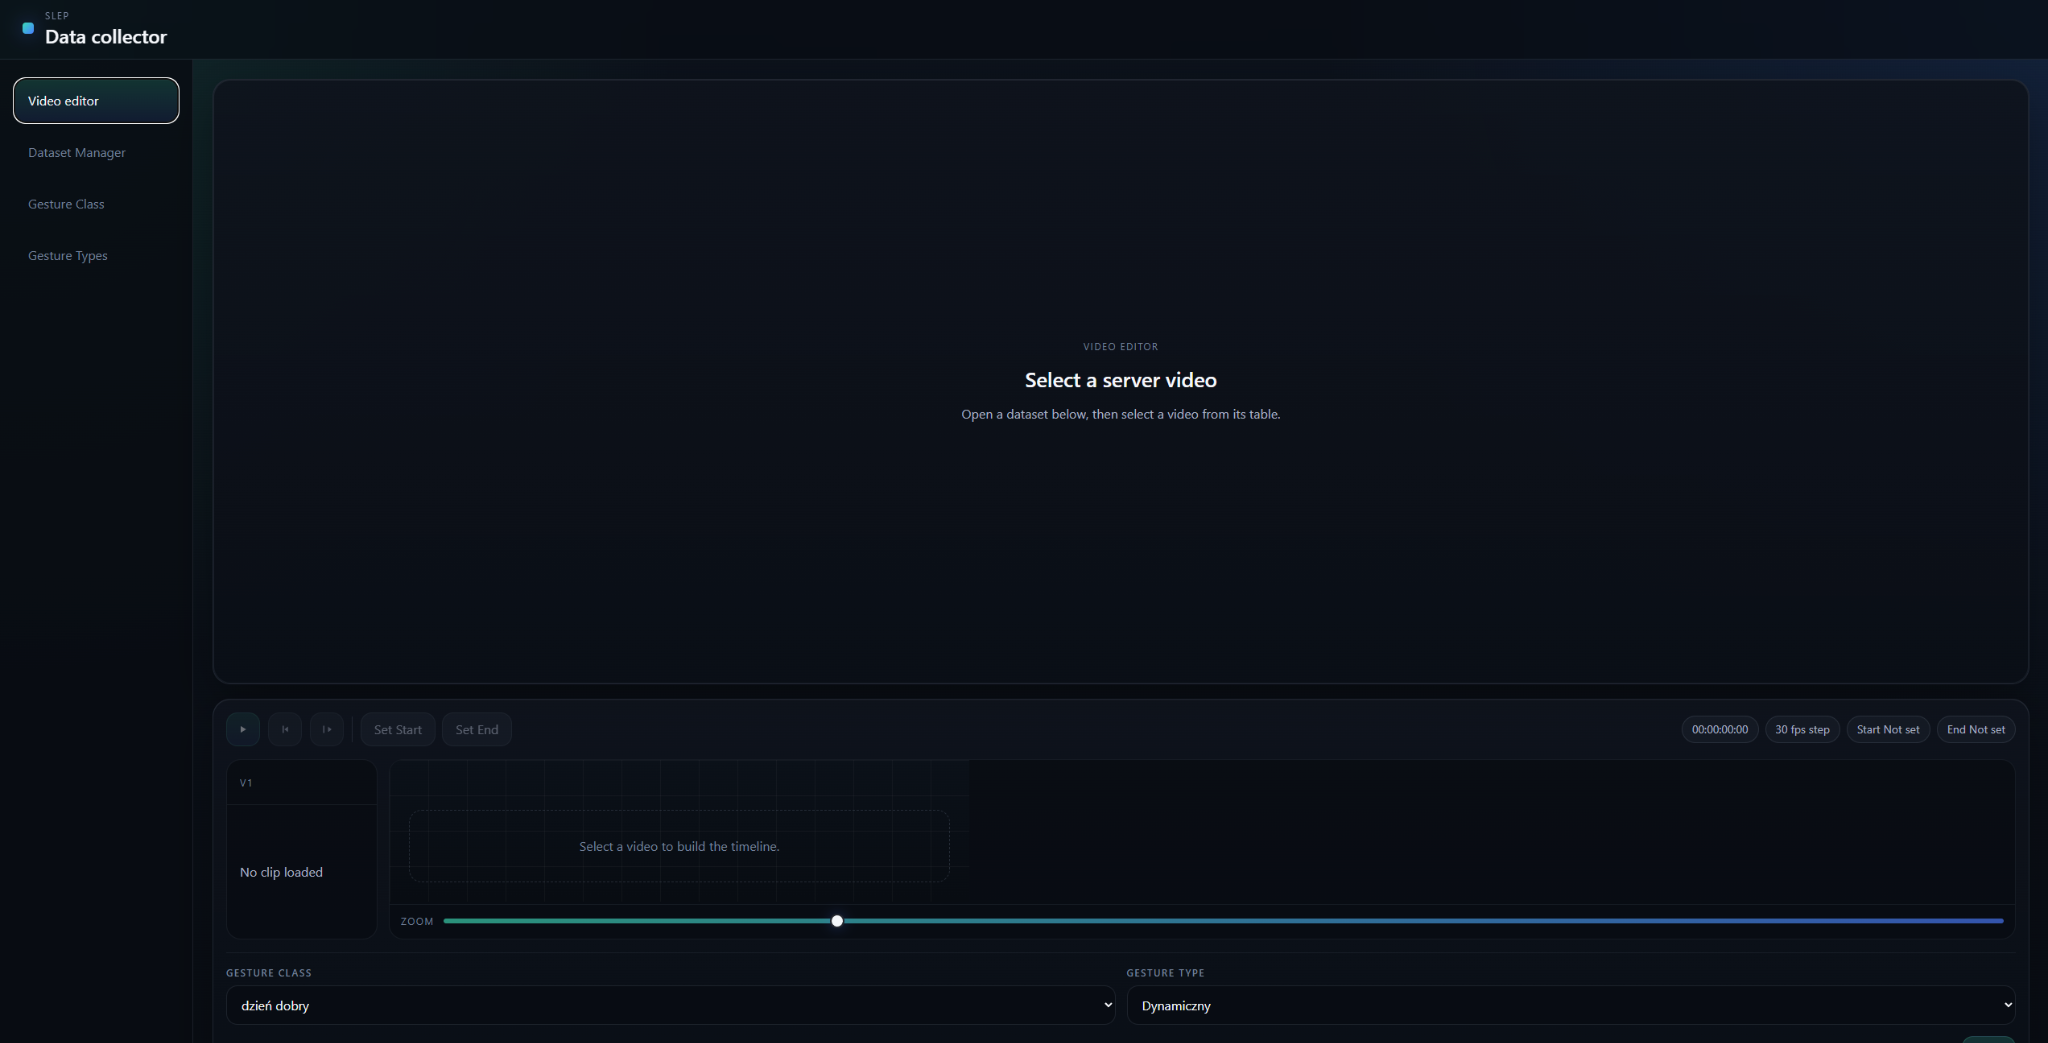
\includegraphics[width=0.85\textwidth]{figures/annotation-platform/video-editor-page.png}
  \caption{Video editor page.}
  \label{fig:video-editor-page}
\end{figure}

\begin{figure}[htbp]
  \centering
  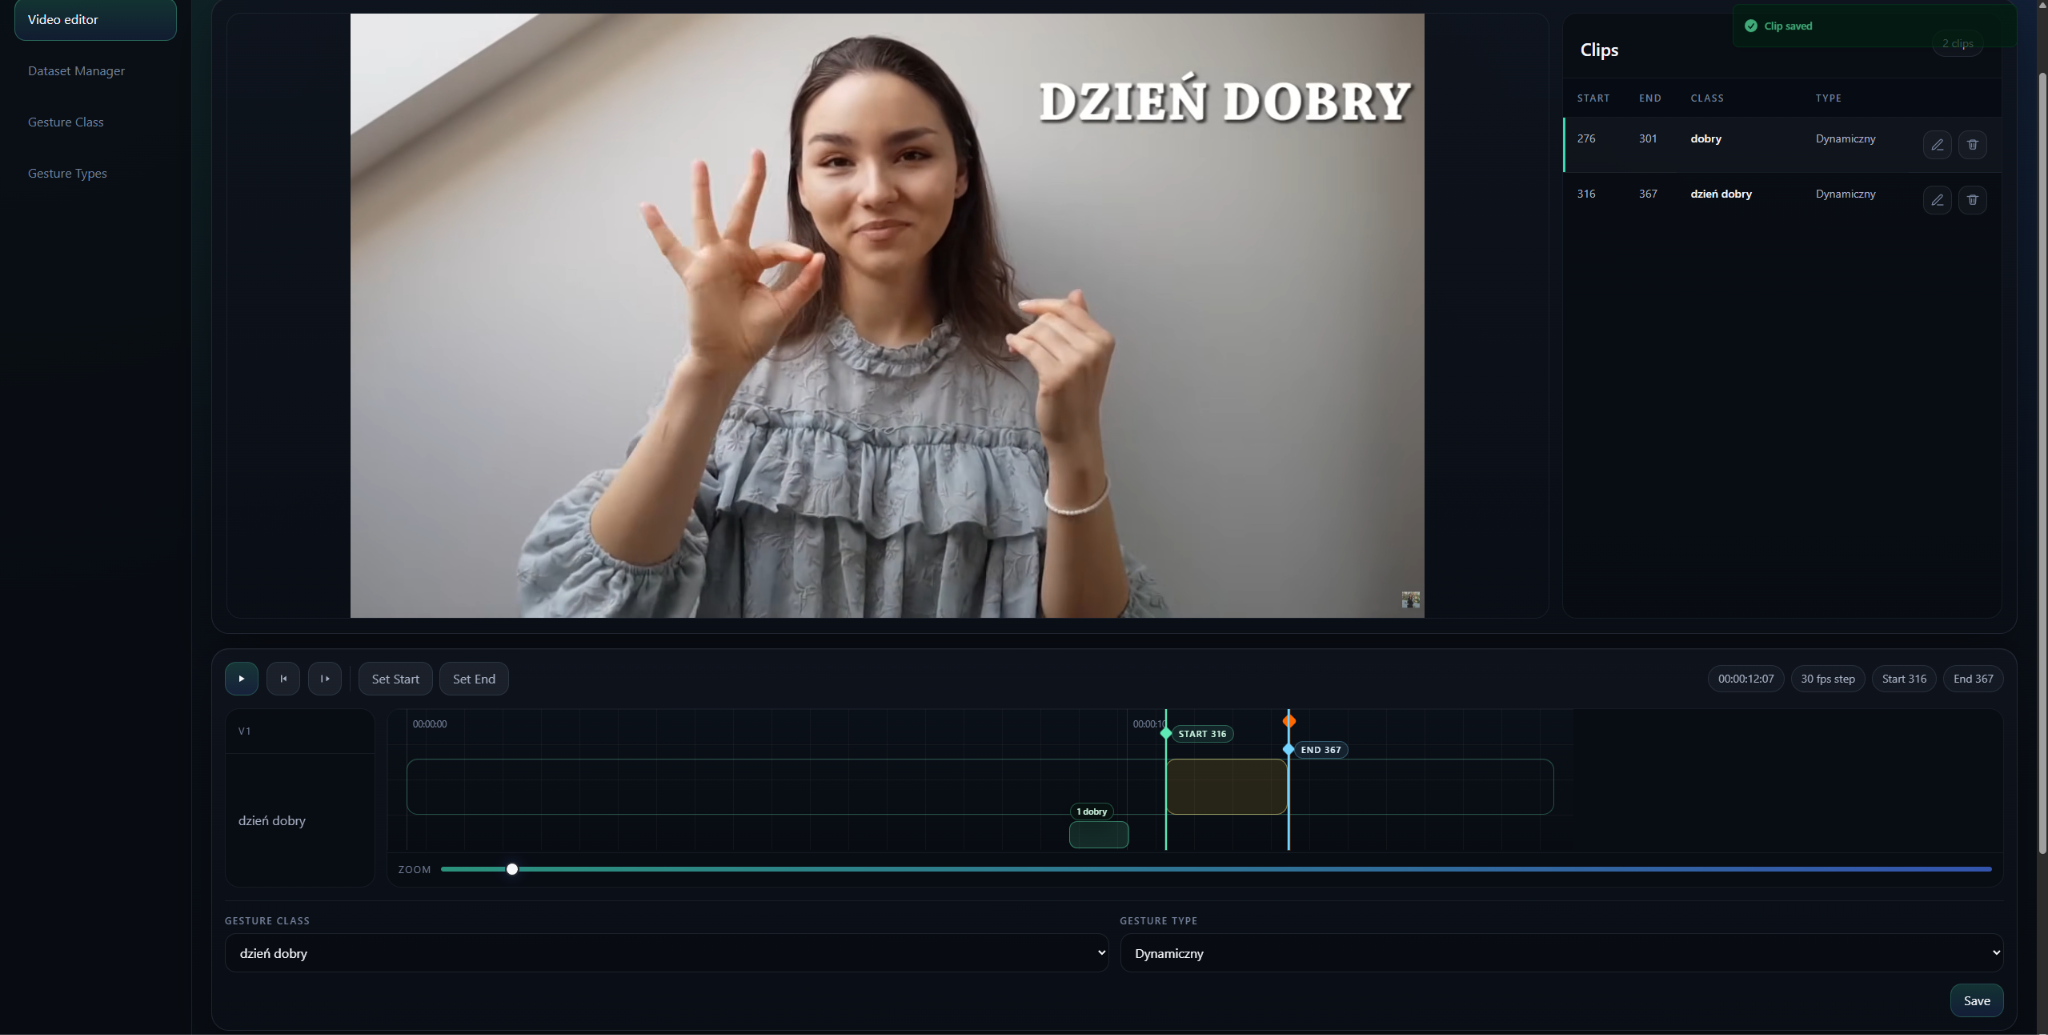
\includegraphics[width=0.85\textwidth]{figures/annotation-platform/video-editor-sample.png}
  \caption{Video editor with a sample video loaded.}
  \label{fig:video-editor-sample}
\end{figure}

\begin{figure}[htbp]
  \centering
  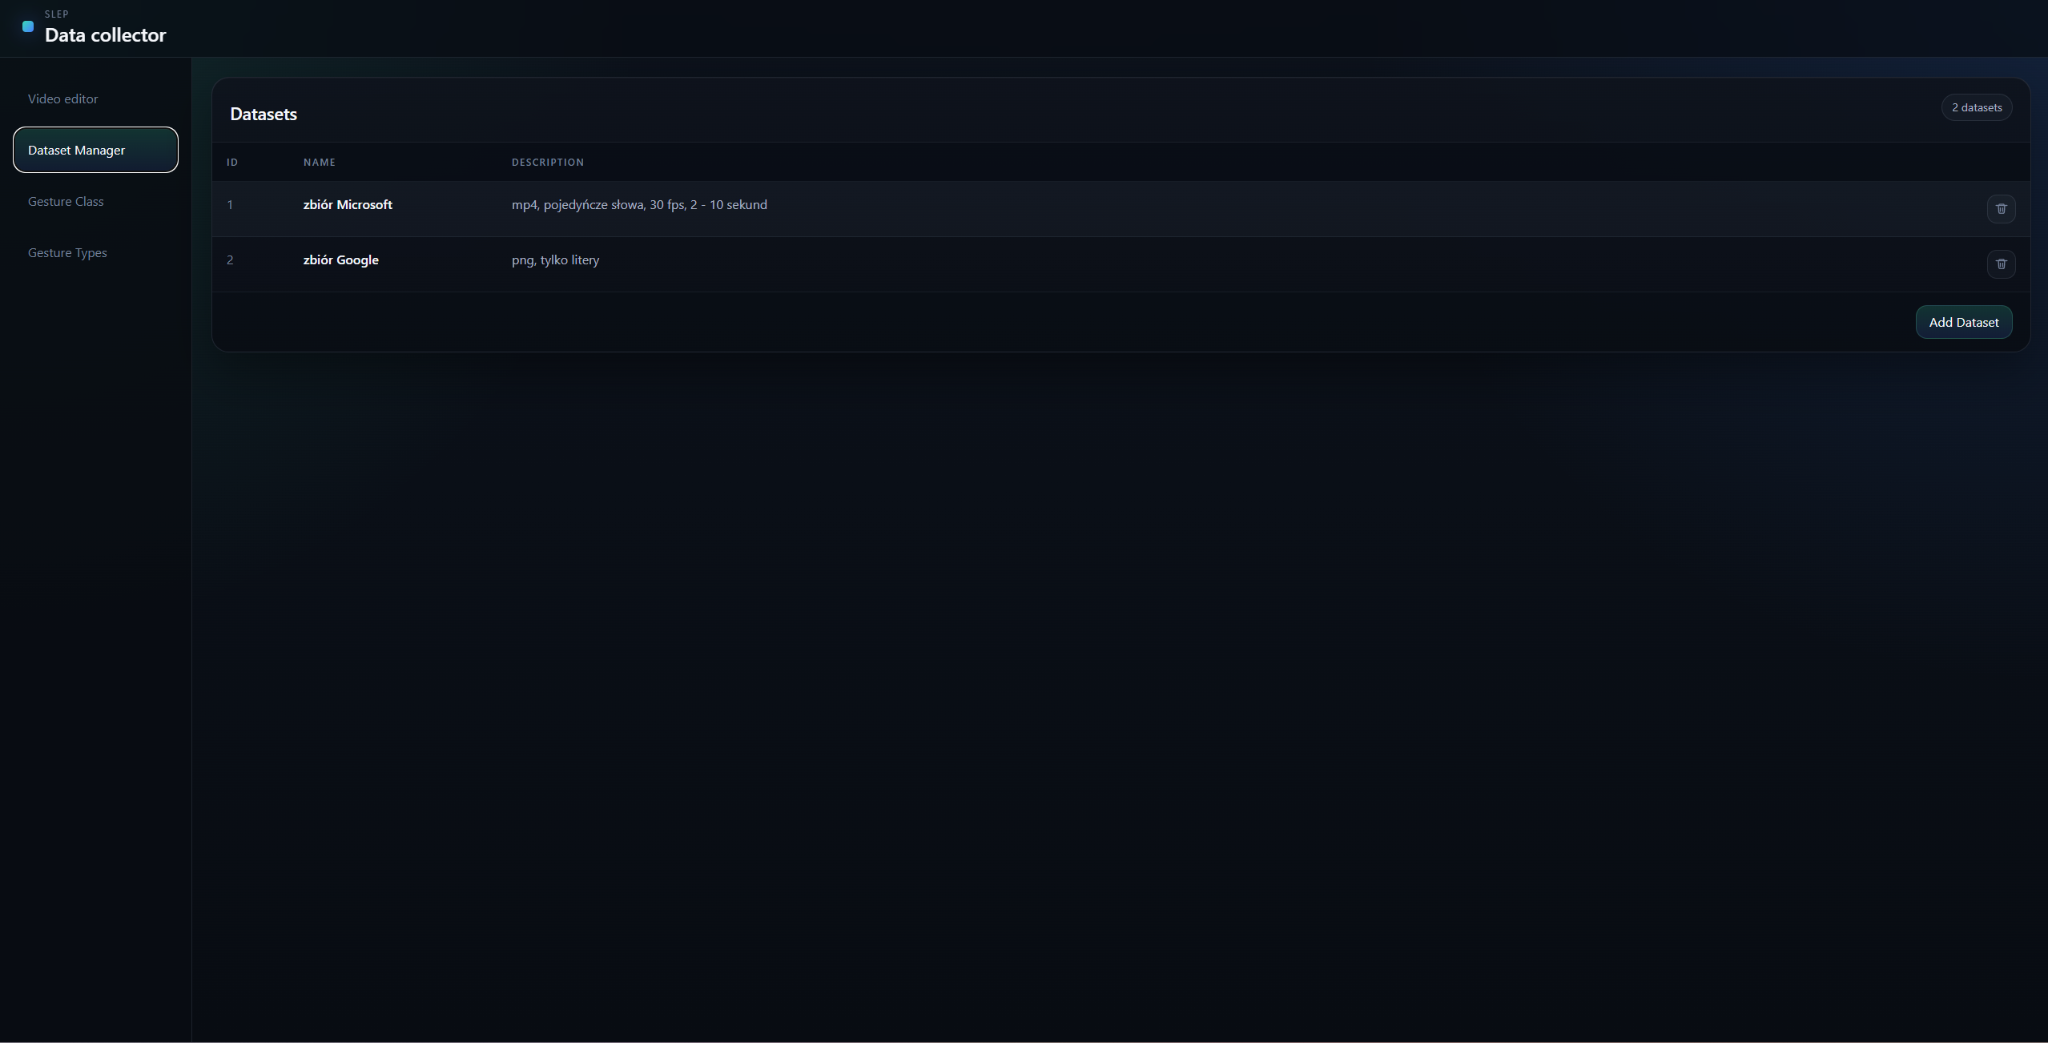
\includegraphics[width=0.7\textwidth]{figures/annotation-platform/dataset-manager-page.png}
  \caption{Dataset Manager page.}
  \label{fig:dataset-manager-page}
\end{figure}

\begin{figure}[htbp]
  \centering
  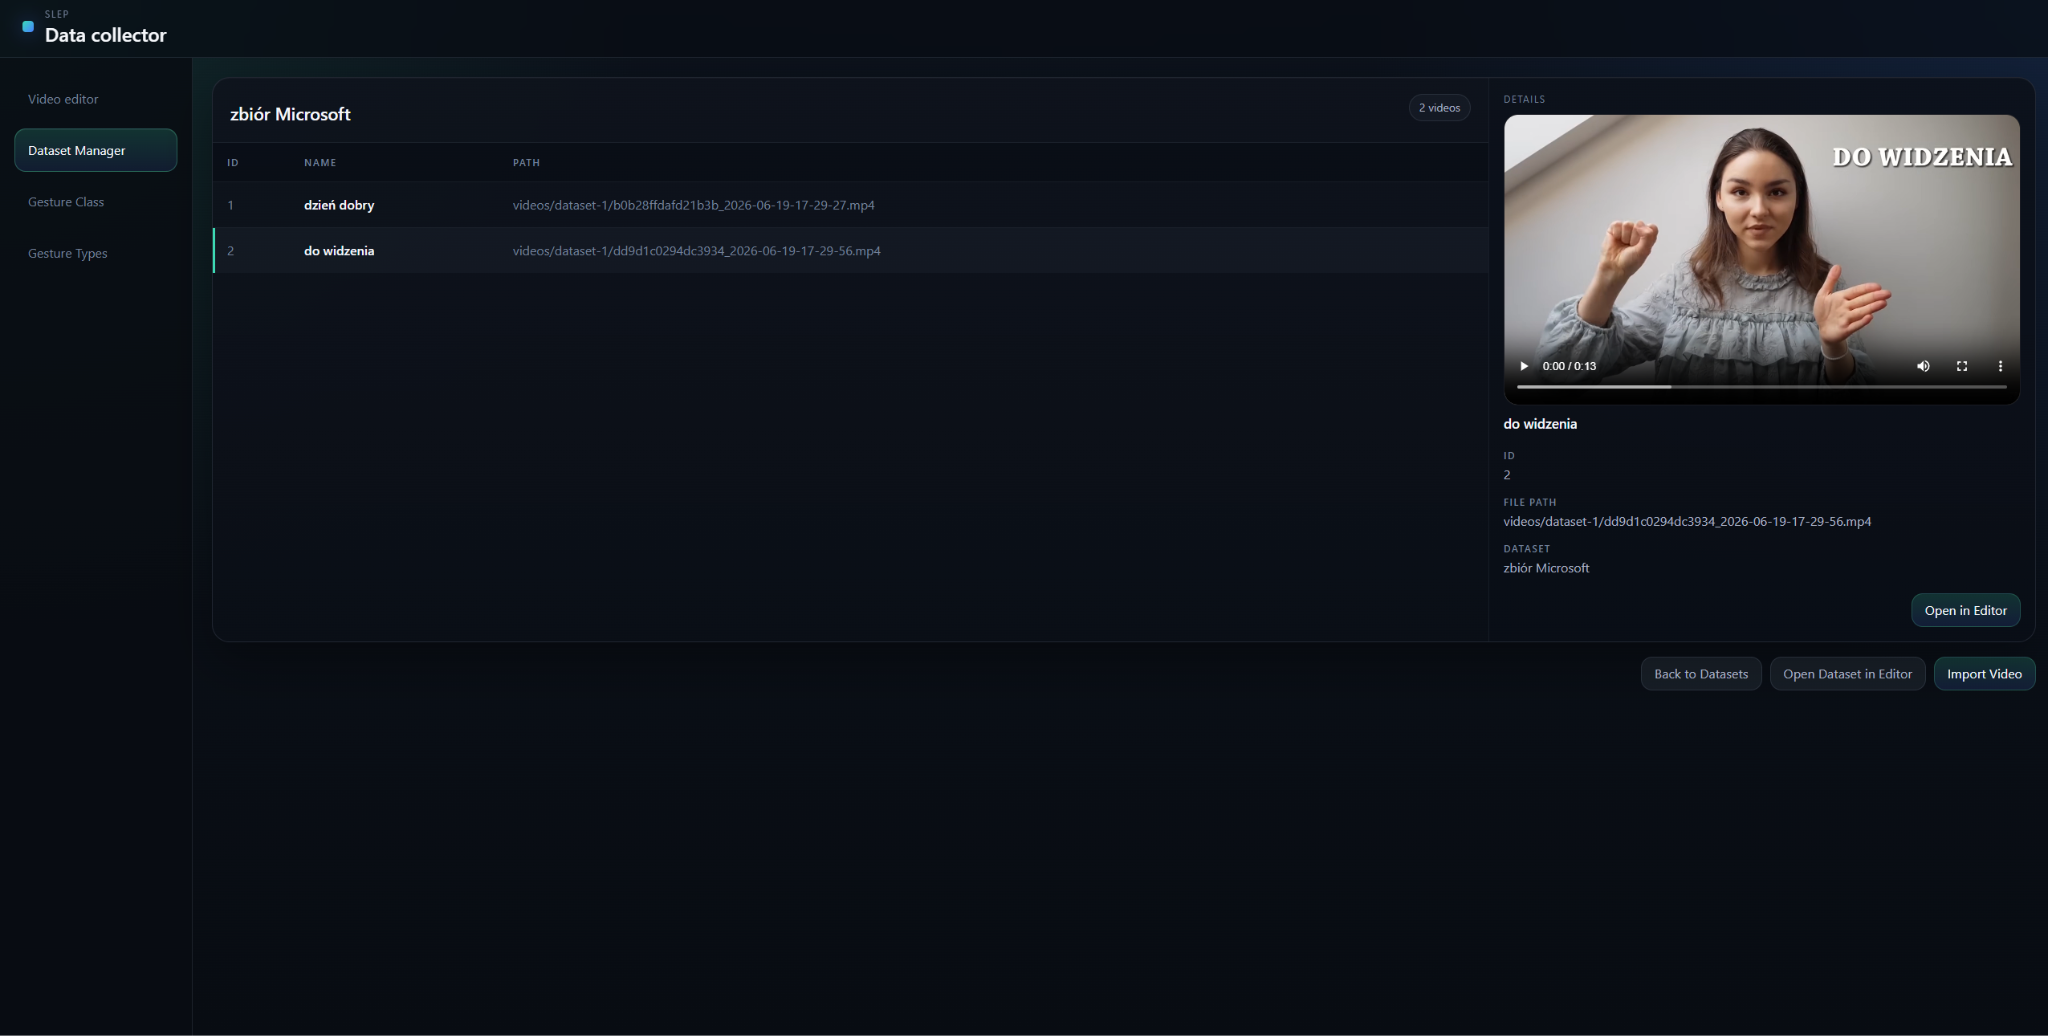
\includegraphics[width=0.85\textwidth]{figures/annotation-platform/dataset-videos-page.png}
  \caption{Dataset Manager's videos page.}
  \label{fig:dataset-videos-page}
\end{figure}

\begin{figure}[htbp]
  \centering
  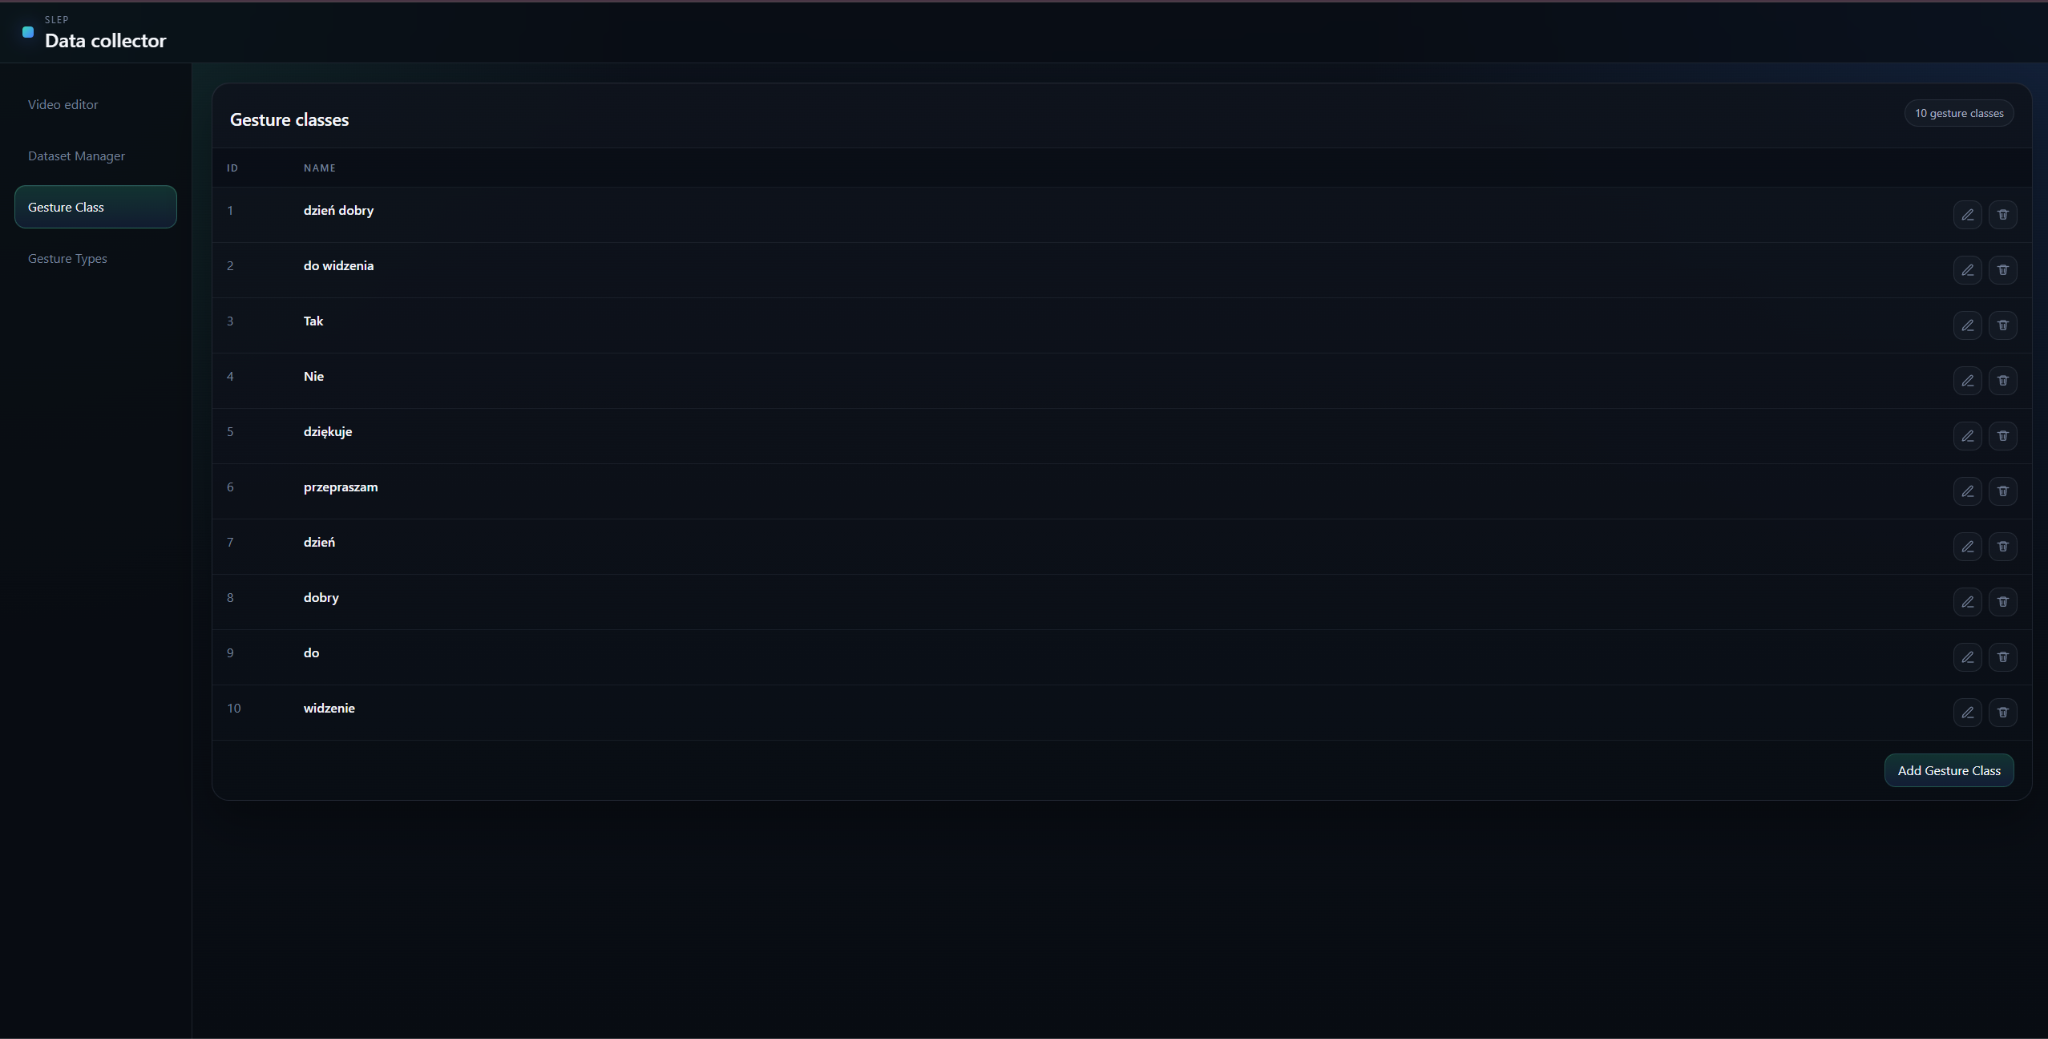
\includegraphics[width=0.7\textwidth]{figures/annotation-platform/gesture-classes-page.png}
  \caption{Gesture classes management page.}
  \label{fig:gesture-classes-page}
\end{figure}

\begin{figure}[htbp]
  \centering
  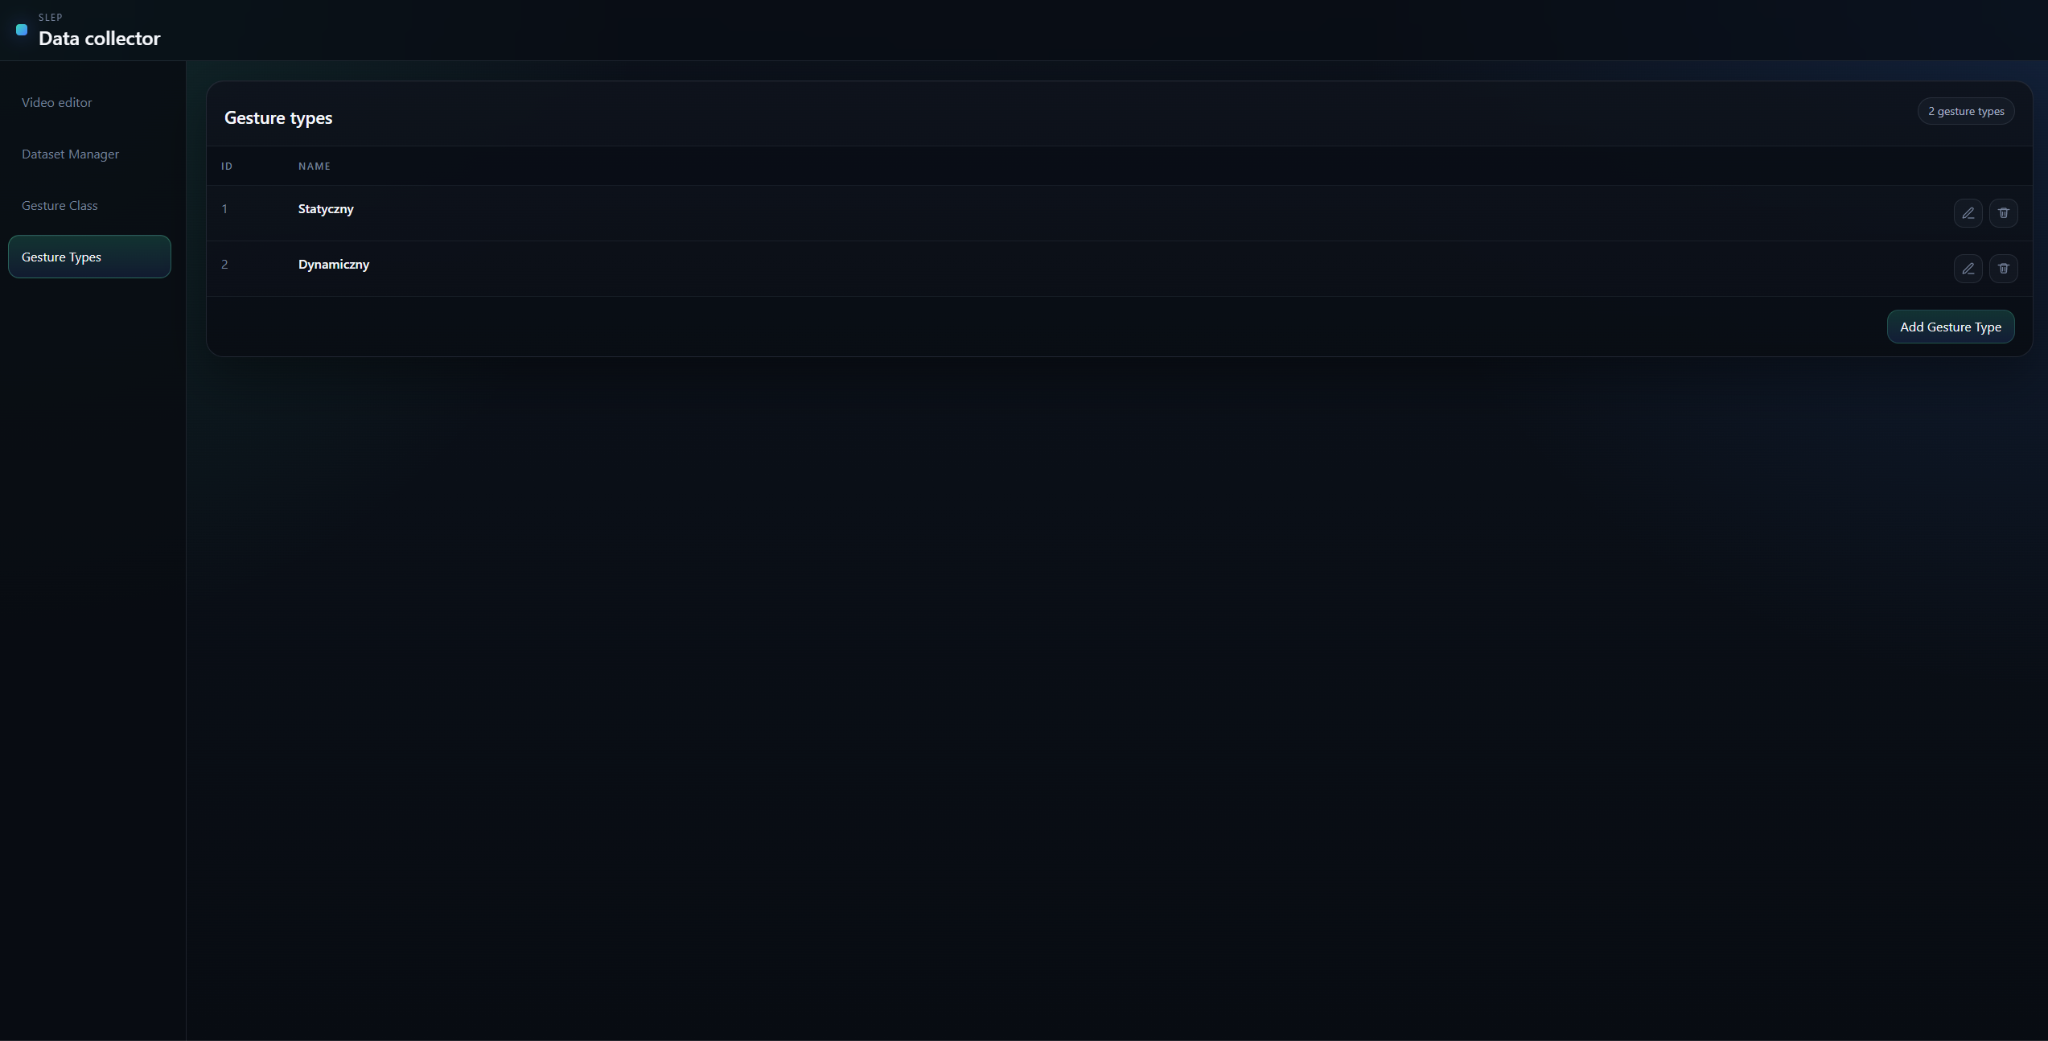
\includegraphics[width=0.7\textwidth]{figures/annotation-platform/gesture-types-page.png}
  \caption{Gesture types management page.}
  \label{fig:gesture-types-page}
\end{figure}

\subsection{System architecture}
\label{sec:annotation-system-architecture}

The application follows a typical full-stack architecture, illustrated in
Figure~\ref{fig:system-architecture}:

\begin{itemize}
  \item the React frontend handles user workflows and communicates with the
        backend through HTTP;
  \item the FastAPI backend exposes REST endpoints for datasets, videos,
        gesture metadata, import jobs, export jobs, and S3 signed URLs;
  \item PostgreSQL stores structured metadata, including datasets, videos,
        clips, landmarks, gesture classes, gesture types, and processing jobs;
  \item MinIO stores large binary files such as uploaded videos and generated
        landmark arrays;
  \item Redis acts as the Celery broker;
  \item Celery workers run long-running video processing tasks outside the
        request-response path.
\end{itemize}

This separation is important because video processing can be computationally
expensive. Uploading a video and requesting an import job returns control to the
web application quickly, while landmark extraction continues in the worker
process.

\begin{figure}[htbp]
  \centering
  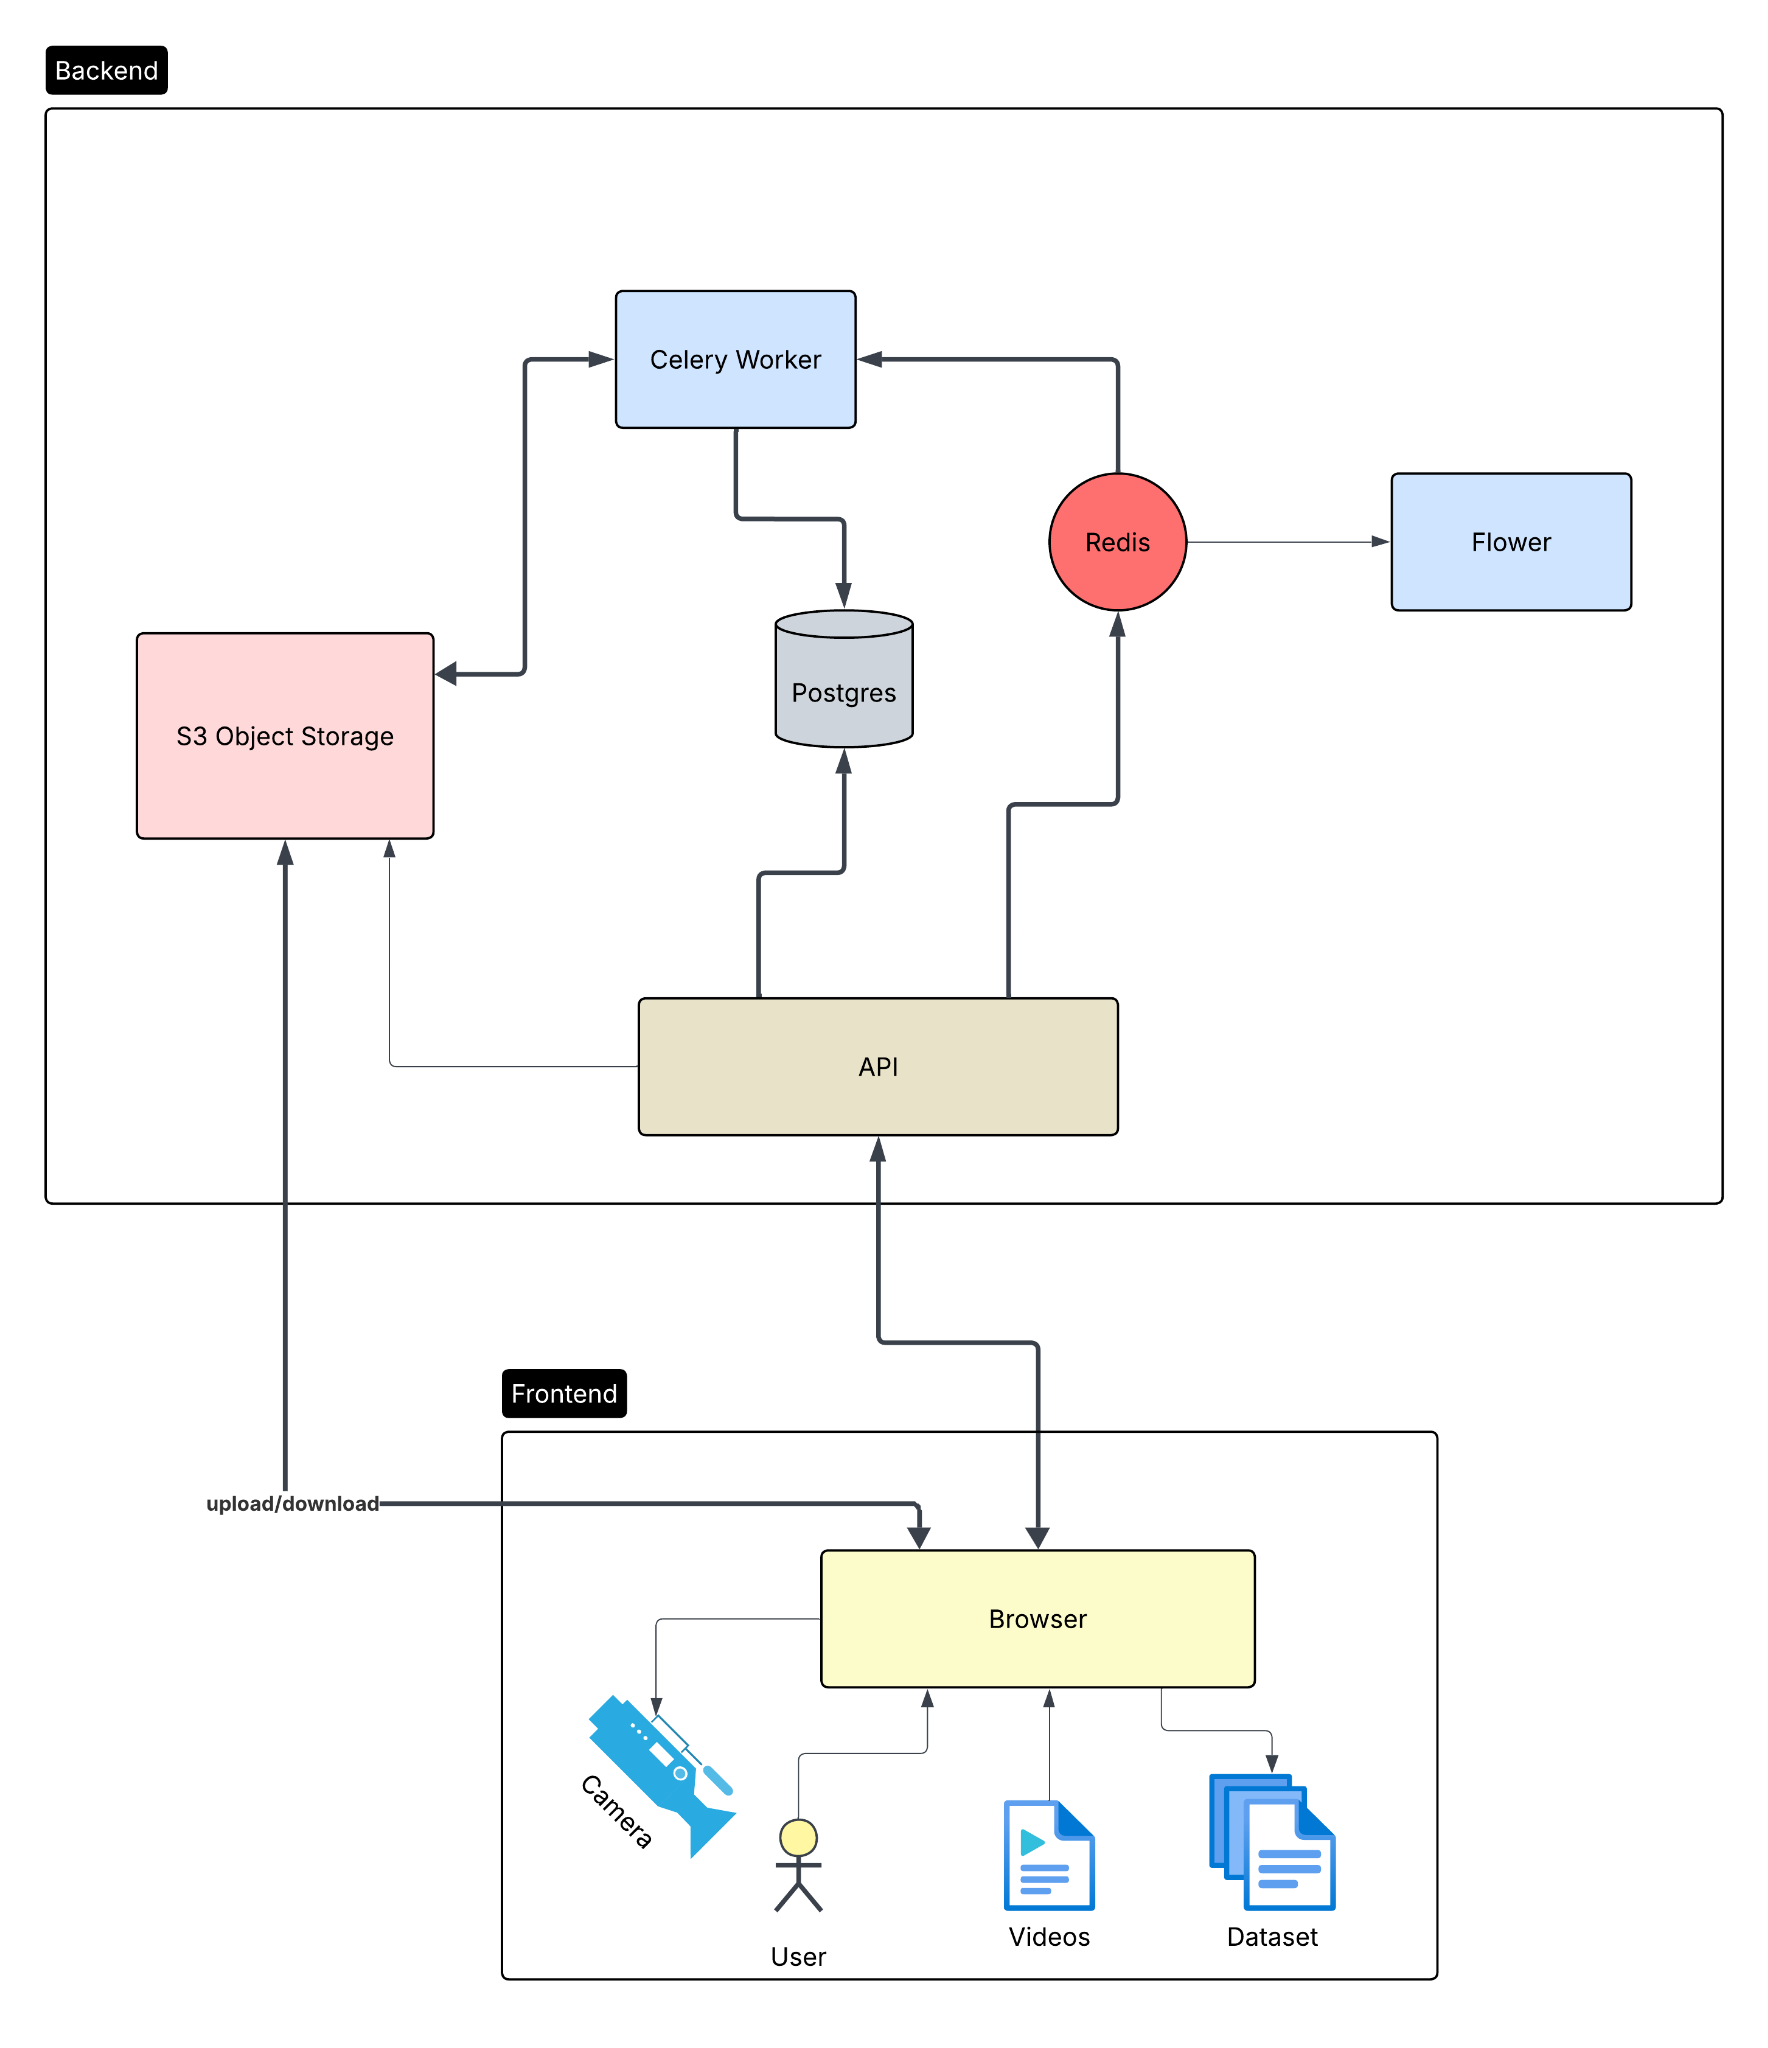
\includegraphics[width=0.85\textwidth]{figures/annotation-platform/system-architecture.png}
  \caption{Diagram of the annotation platform's system architecture.}
  \label{fig:system-architecture}
\end{figure}

The backend is implemented with Python~3.12, FastAPI, Pydantic, SQLAlchemy
async, Alembic, PostgreSQL, Redis, Celery, MinIO/S3, and MediaPipe. It exposes
REST endpoints under \texttt{/api/v1} and uses asynchronous database access for
application requests. It is organised around API routers, CRUD modules,
services, schemas, and SQLAlchemy models (Figure~\ref{fig:backend-structure}),
and implements the following API areas:

\begin{itemize}
  \item \textbf{datasets}: create, list, read, update, and delete datasets;
  \item \textbf{videos}: list videos, filter videos by dataset, read video
        details, update videos, delete videos, and manage related clips and
        landmarks;
  \item \textbf{gesture classes}: create, list, read, update, and delete
        gesture classes;
  \item \textbf{gesture types}: create, list, read, update, and delete gesture
        types;
  \item \textbf{import video jobs}: create and inspect video import jobs;
  \item \textbf{S3 integration}: generate signed upload and download URLs;
  \item \textbf{exported datasets and export dataset jobs}: database and API
        structures for future dataset export workflows.
\end{itemize}

\begin{figure}[htbp]
  \centering
  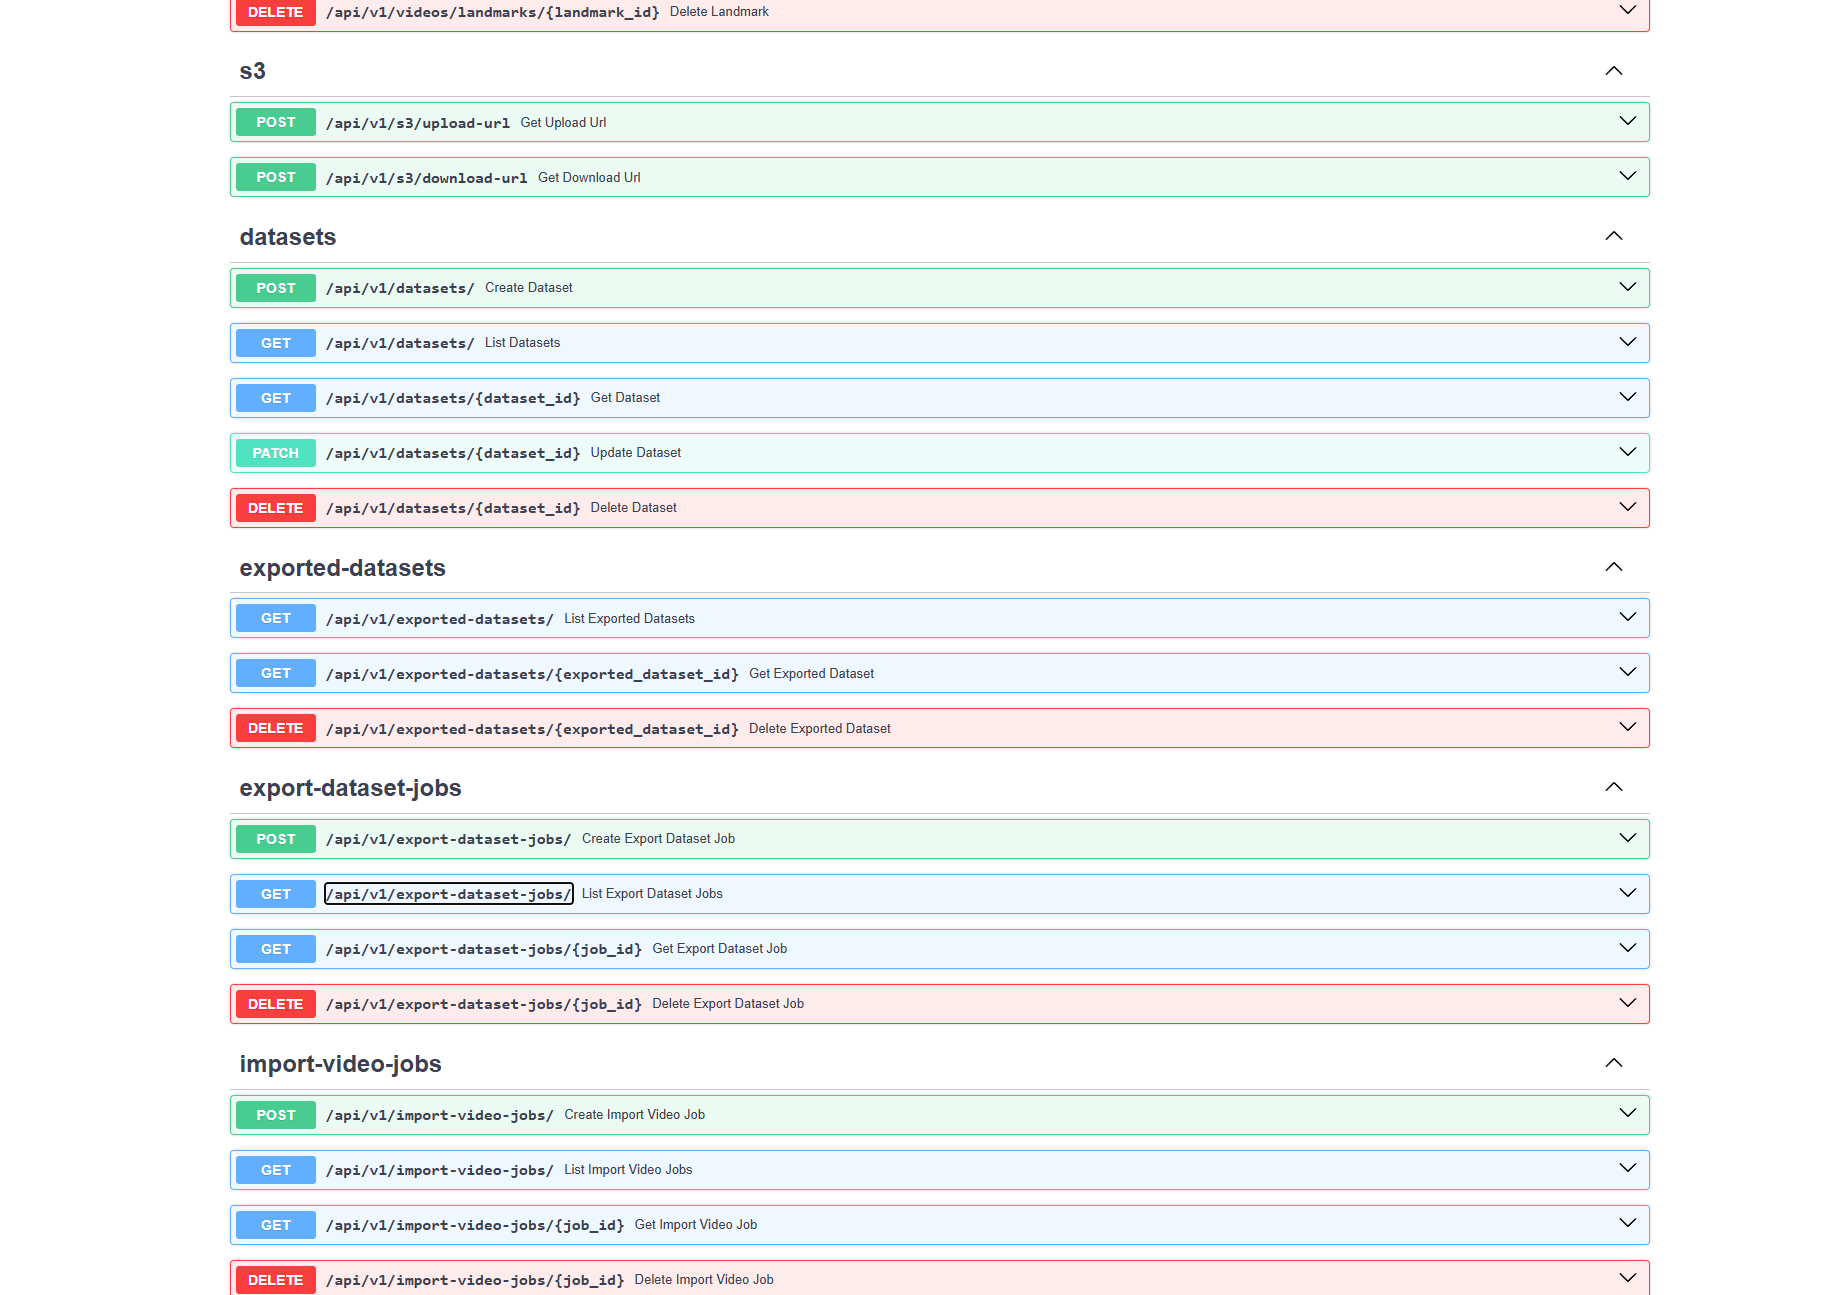
\includegraphics[width=0.7\textwidth]{figures/annotation-platform/swagger-ui.png}
  \caption{Backend API, Swagger UI.}
  \label{fig:swagger-ui}
\end{figure}

The import workflow is handled through \texttt{VideoService} and a Celery task.
When a video import job is created, the backend stores the job metadata and
dispatches a Celery task. The worker downloads the video from MinIO, extracts
landmarks, saves the result as a NumPy \texttt{.npy} file, uploads it back to
MinIO, creates a video record, and links the generated landmark file to that
video. The upload flow itself is implemented through signed S3 URLs: the
frontend asks the backend for an upload URL, uploads the selected file directly
to MinIO, and then creates an import job that references the uploaded object
path. This avoids sending large video files through the FastAPI application
process.

Video analysis is carried out asynchronously by a Celery worker
(task \texttt{process\_video}). The heart of the process is the
\texttt{LandmarkExtractionService}, which uses Google's MediaPipe Holistic and
proceeds as follows:

\begin{enumerate}
  \item \textbf{File retrieval} -- the service downloads the video file from
        the specified S3 key to the local worker environment;
  \item \textbf{ML network initialisation} -- the MediaPipe Holistic detector
        (\texttt{HolisticLandmarker}) is started via a context manager;
  \item \textbf{Frame-level extraction} -- detection runs on each video frame
        to extract spatial $x$, $y$, and $z$ coordinates;
  \item \textbf{Vectorisation} -- results for all components (face, body,
        hands) are combined into one flat vector, detailed in
        Section~\ref{sec:annotation-data-format};
  \item \textbf{Matrix aggregation} -- frame vectors are sequentially appended
        to a list, which ultimately becomes a 2D matrix of shape
        [number of frames $\times$ number of features];
  \item \textbf{Export to S3} -- the matrix is serialised as a \texttt{.npy}
        file (\texttt{numpy.save()}) and then uploaded to S3;
  \item \textbf{Database confirmation} -- a record is created in the
        \texttt{landmarks} table with the S3 key.
\end{enumerate}

For every frame, the landmark extraction service stores pose, face, left-hand,
and right-hand landmark coordinates in a fixed-size row; missing detections are
represented with zeros, which keeps the output array shape consistent across
frames and simplifies later machine learning use
(Figure~\ref{fig:annotation-methodology}).

\begin{figure}[htbp]
  \centering
  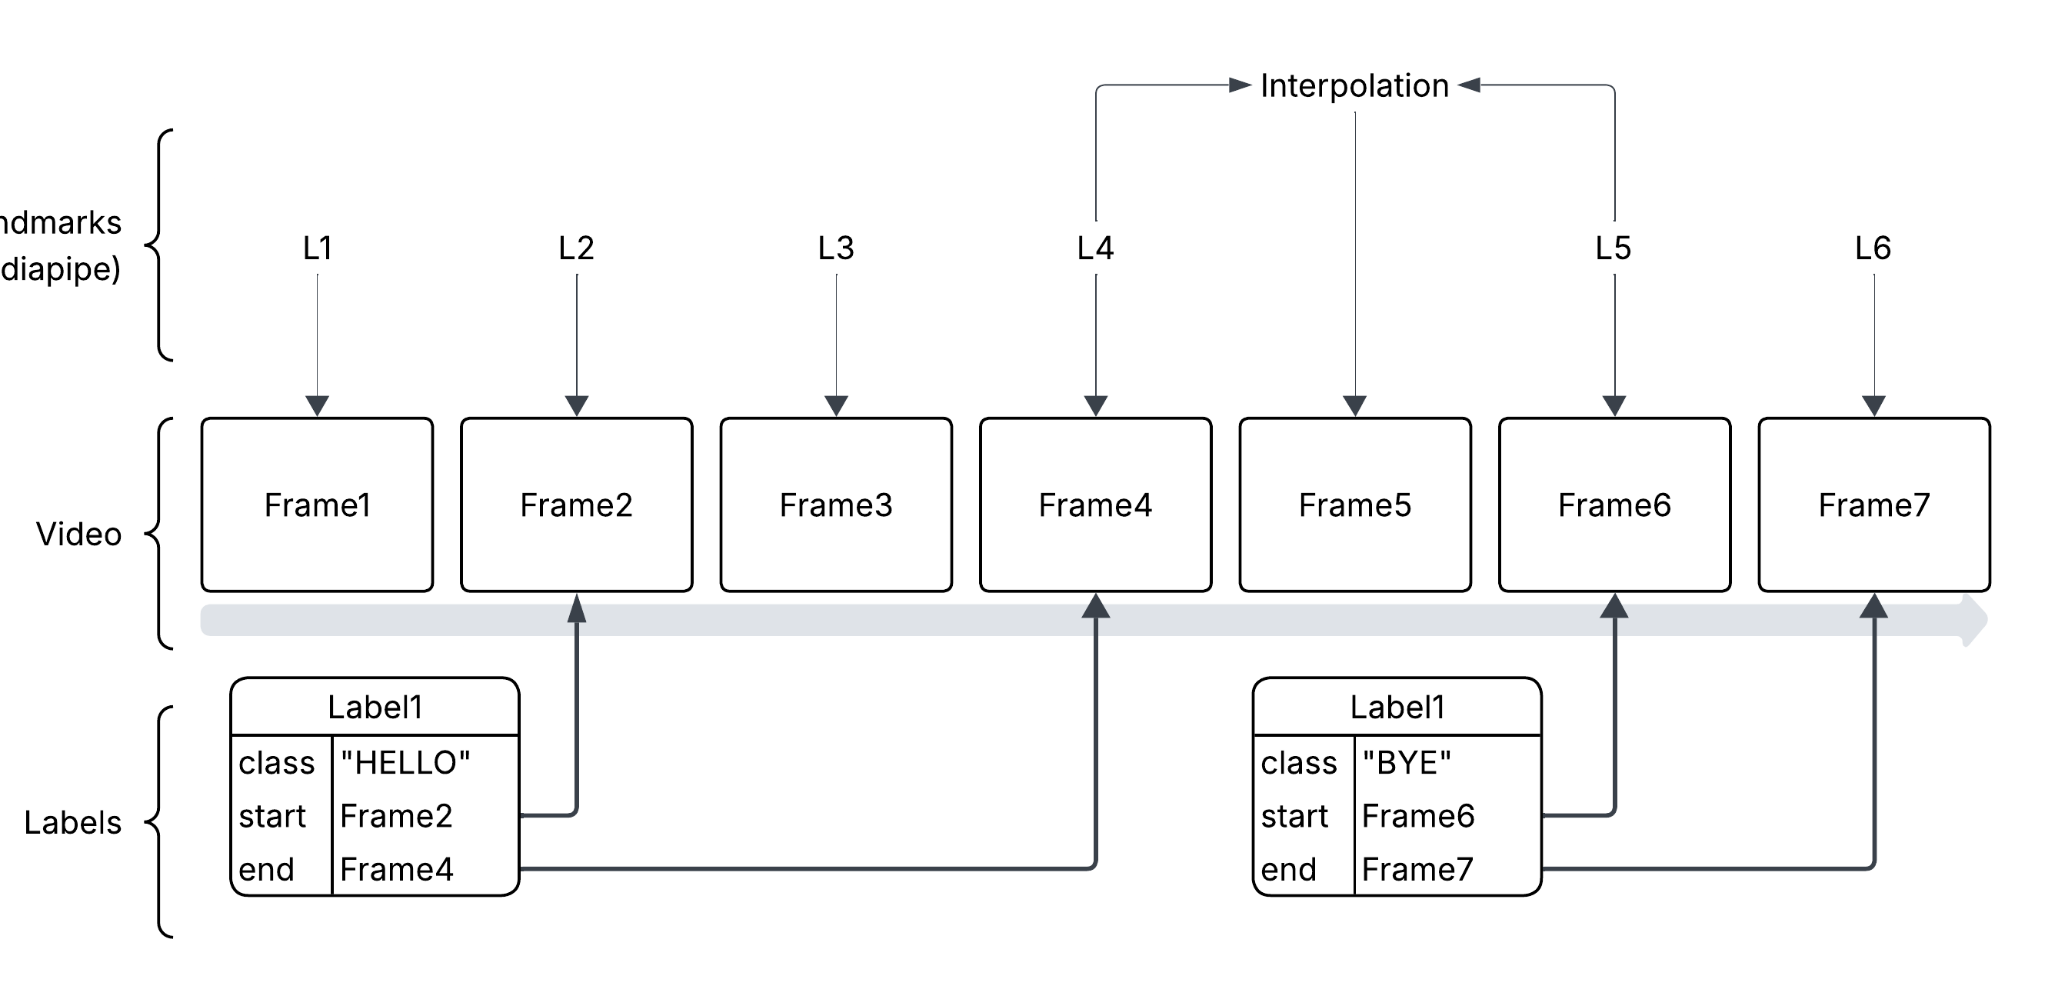
\includegraphics[width=0.85\textwidth]{figures/annotation-platform/annotation-methodology.png}
  \caption{Video-gloss annotation methodology.}
  \label{fig:annotation-methodology}
\end{figure}

The current database model contains the following main entities:

\begin{itemize}
  \item \textbf{Dataset} -- a named collection of related videos;
  \item \textbf{Video} -- metadata for a stored video, including file path,
        description, FPS, duration, and dataset relation;
  \item \textbf{Landmark} -- metadata for generated landmark files associated
        with videos;
  \item \textbf{Clip} -- an annotated frame range within a video;
  \item \textbf{GestureClass} -- a label category assigned to clips;
  \item \textbf{GestureType} -- an additional gesture classification assigned
        to clips;
  \item \textbf{ImportVideoJob} -- processing state for video import and
        landmark extraction;
  \item \textbf{ExportDatasetJob} -- processing state for future dataset export
        tasks;
  \item \textbf{ExportedDataset} -- metadata describing generated exported
        datasets.
\end{itemize}

The relationship between videos, clips, landmarks, gesture classes, and gesture
types creates a structured annotation layer over raw video data, suitable for
later dataset export and model training preparation. Key architectural
decisions made in the data model include:

\begin{itemize}
  \item \texttt{ON DELETE CASCADE} for related records (e.g.\ clips, landmarks,
        export dataset jobs) when the parent entity is deleted, eliminating
        orphaned data;
  \item \texttt{ON DELETE SET NULL} from datasets to videos: deleting a dataset
        does not delete its videos, it only sets \texttt{dataset\_id} to
        \texttt{NULL}, preserving valuable video data;
  \item \texttt{ENUM} types for job statuses (\texttt{in\_queue},
        \texttt{processing}, \texttt{done}, \texttt{error}), enforcing data
        consistency;
  \item denormalisation in \texttt{exported\_datasets}: dataset name and
        description are copied at export time, so the snapshot is immutable and
        the historical state of the dataset is always reproducible;
  \item separation of processing logic (\texttt{import\_video\_jobs},
        \texttt{export\_dataset\_jobs}) from business data (videos, clips,
        landmarks);
  \item separation of gesture semantics into \texttt{gesture\_classes} (general
        categories) and \texttt{gesture\_types} (specific types), allowing more
        flexible data modelling;
  \item nullable job fields (\texttt{video\_id}, \texttt{error\_message},
        \texttt{dataset\_id}, \texttt{exported\_dataset\_id}), allowing
        incremental record population during processing;
  \item no soft-delete mechanism: deleting an entity is a physical and
        irreversible operation.
\end{itemize}

The project includes Docker Compose services for the full development
environment: \texttt{postgres} for relational metadata storage, \texttt{redis}
for Celery queue communication, \texttt{s3-dev}/\texttt{s3} for MinIO object
storage, \texttt{data-collection-api} for the FastAPI backend,
\texttt{data-collection-worker} for background Celery processing,
\texttt{data-collection-flower} for monitoring Celery workers, and
\texttt{data-collection-frontend} for serving the frontend build through Nginx.
The frontend keeps API types and request functions in a shared actions module,
while pages and components focus on user workflows
(Figure~\ref{fig:frontend-structure}); the backend separates routers, schemas,
CRUD operations, services, models, and worker tasks
(Figure~\ref{fig:backend-structure}). Alembic migrations are present for
database schema evolution.

\begin{figure}[htbp]
  \centering
  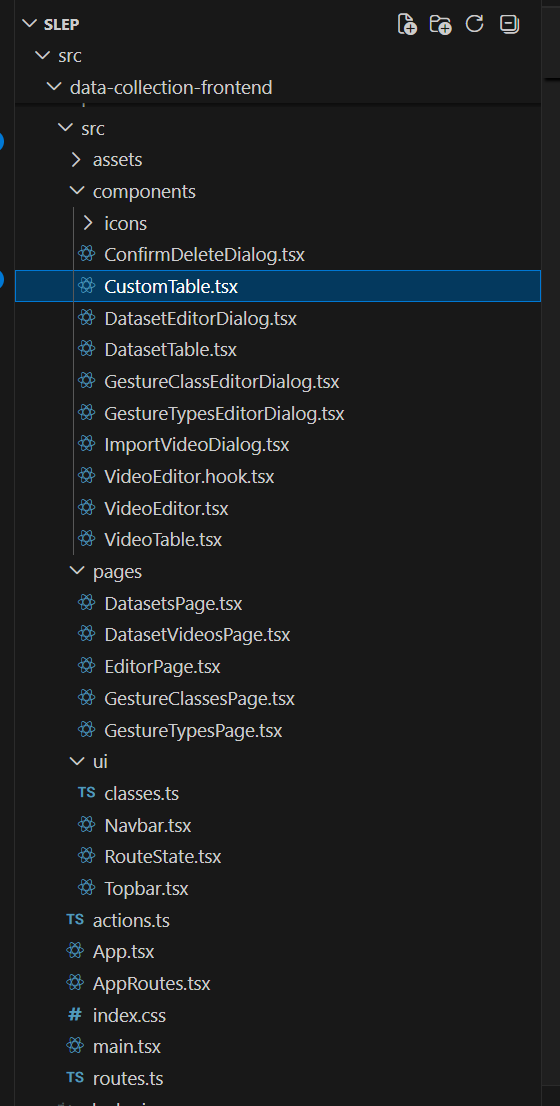
\includegraphics[width=0.6\textwidth]{figures/annotation-platform/frontend-structure.png}
  \caption{Frontend project structure.}
  \label{fig:frontend-structure}
\end{figure}

\begin{figure}[htbp]
  \centering
  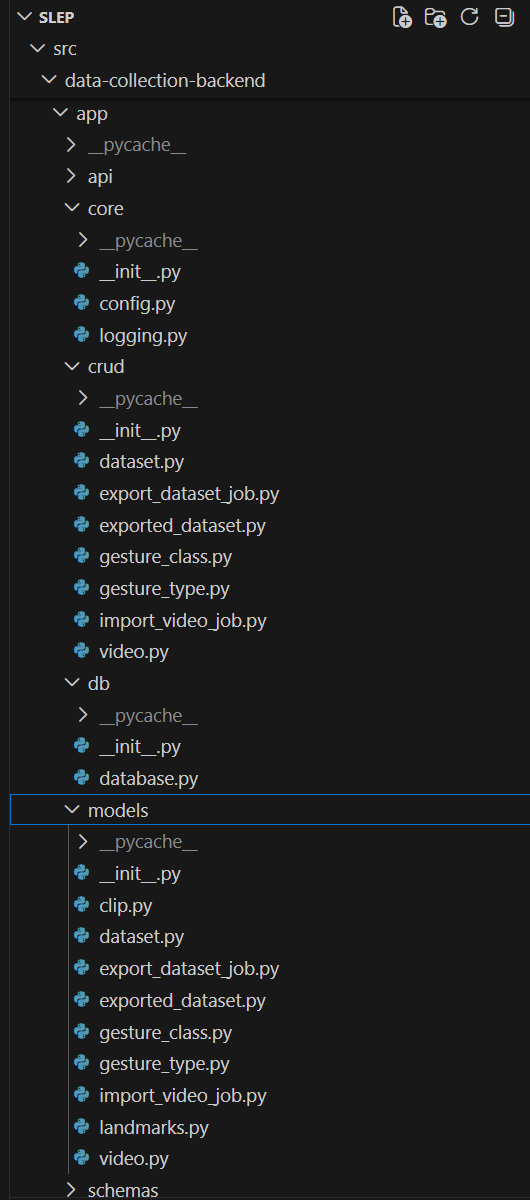
\includegraphics[width=0.5\textwidth]{figures/annotation-platform/backend-structure.png}
  \caption{Backend project structure.}
  \label{fig:backend-structure}
\end{figure}

\subsection{Data format and structure}
\label{sec:annotation-data-format}

Landmark files are stored in Amazon S3 as binary NumPy matrices (\texttt{.npy}).
Videos are addressed by an arbitrary S3 key, and their corresponding landmark
file uses the same key with a \texttt{\_landmarks.npy} suffix. Each \texttt{.npy}
file contains a 2D matrix with dimensions [number of video frames]
$\times$ [1659], as summarised in Table~\ref{tab:landmark-vector}.

\begin{table}[htbp]
  \centering
  \caption{Structure of the per-frame landmark feature vector (1659 values).}
  \label{tab:landmark-vector}
  \begin{tabular}{lccc}
    \hline
    \textbf{Component} & \textbf{Index range} & \textbf{Points} & \textbf{Values ($x,y,z$)} \\
    \hline
    Pose (silhouette) & 0--98    & 33  & 99   \\
    Face              & 99--1532 & 478 & 1434 \\
    Left hand         & 1533--1595 & 21 & 63  \\
    Right hand        & 1596--1658 & 21 & 63  \\
    \hline
    \textbf{Total}    & --       & 553 & 1659 \\
    \hline
  \end{tabular}
\end{table}

If a given element is not detected in a given frame (e.g.\ a missing right
hand), all of its assigned values are set to $0.0$. The resulting per-frame
representation -- one row per video frame, 1659 float32 columns per row -- is
the same landmark representation consumed by the preprocessing pipeline of the
isolated gloss recognition model described in
Section~\ref{sec:gloss-recognition-preprocessing}.

The end-to-end data flow through the platform proceeds in three stages:

\begin{enumerate}
  \item \textbf{Video import} -- a record is created in
        \texttt{import\_video\_jobs} with status \texttt{in\_queue}; the status
        is updated to \texttt{processing}; the file is downloaded and its
        metadata (FPS, duration) extracted; a record is created in
        \texttt{videos}; the job status is finally updated to \texttt{done}
        (with \texttt{video\_id} filled) or \texttt{error} (with
        \texttt{error\_message} filled);
  \item \textbf{Video processing (landmark extraction)} -- the Celery worker
        downloads the video from S3, runs MediaPipe Holistic on each frame,
        generates the landmark matrix and saves it to S3, creates a record in
        \texttt{landmarks}, and creates records in \texttt{clips} with
        \texttt{gesture\_class\_id} and \texttt{gesture\_type\_id} assignment;
  \item \textbf{Dataset export} -- a record is created in
        \texttt{export\_dataset\_jobs} with status \texttt{in\_queue}; the
        worker generates a data package (video and landmarks) for all videos in
        the dataset; a record is generated in \texttt{exported\_datasets} (with
        denormalised dataset data); the task status is updated to \texttt{done}
        or \texttt{error}.
\end{enumerate}

At the current stage, the project has a functional foundation for video dataset
management and annotation, supporting the complete path from dataset creation,
through video upload, to background landmark extraction and clip annotation.
The most developed areas are the backend CRUD and REST API structure, local
service orchestration with Docker Compose, S3-compatible video upload,
asynchronous landmark extraction through Celery, dataset and gesture taxonomy
management in the UI, and timeline-based clip annotation in the browser. The
dataset export workflow has database models, schemas, CRUD modules, and API
endpoints, but the asynchronous export processing pipeline still needs to be
completed, and import job status updates should be made more explicit throughout
the worker lifecycle.

Known limitations of the current platform include: video metadata such as FPS
and duration is currently stored with fixed values in the worker instead of
being fully derived from the uploaded file; the frontend API base URL is
hardcoded rather than configurable; authentication and authorisation are not
implemented; validation around clip ranges, duplicate labels, and dataset
consistency can be expanded; and landmark preview generation is modelled but not
fully implemented. Automated test coverage is also limited; the most important
future test areas are API endpoint behaviour, worker behaviour for successful
and failed imports, database migration validation, frontend editor behaviour for
frame selection and clip saving, and integration testing of the full
upload-import-processing path. These limitations do not prevent local data
collection experiments, but should be addressed before the platform is used as a
robust production or research data platform.

\todo{PLACEHOLDER: Insert an entity-relationship diagram summarising the
\texttt{datasets} / \texttt{videos} / \texttt{clips} / \texttt{landmarks} /
\texttt{gesture\_classes} / \texttt{gesture\_types} / \texttt{import\_video\_jobs}
/ \texttt{export\_dataset\_jobs} / \texttt{exported\_datasets} schema and its
foreign-key relationships.}

%%%%%%%%%%%%%%%%%%%%%%%%%%%%%%%%%%%%%%%%%%%%%%%%%%%%%%%%%%%%%%
%% Chapter 4: Isolated Gloss Recognition (video2gloss)
%%%%%%%%%%%%%%%%%%%%%%%%%%%%%%%%%%%%%%%%%%%%%%%%%%%%%%%%%%%%%%

\section{Isolated Gloss Recognition (video2gloss)}
\label{chap:isolated-gloss-recognition}

To address the video-to-gloss task introduced in
Chapter~\ref{chap:related-work}, we adopt a retrieval-based paradigm: rather
than learning a fixed set of class boundaries, we learn an embedding space in
which examples of the same gloss cluster together, and defer classification to
nearest-neighbour retrieval within that space
(Figure~\ref{fig:slt-problem-overview}). This formulation handles intra-class
spread more gracefully than a softmax classifier, scales naturally to new
vocabulary without retraining the classifier head, and provides a
representational backbone amenable to the alignment-based and
continuous-recognition extensions discussed in
Section~\ref{sec:gloss-recognition-discussion}.

\begin{figure}[htbp]
  \centering
  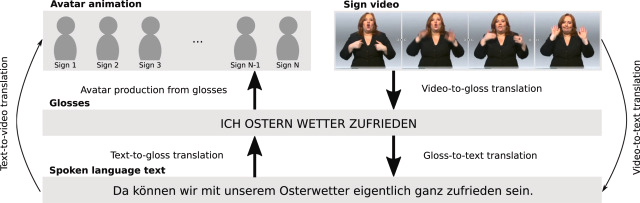
\includegraphics[width=0.85\textwidth]{figures/gloss-recognition/slt-problem-overview.png}
  \caption{The general problem of sign language translation and the position of
  the video-to-gloss task within it.}
  \label{fig:slt-problem-overview}
\end{figure}

This chapter's contributions are: (i) a retrieval-based formulation of isolated
video-to-gloss recognition, casting gloss recognition as metric learning
followed by nearest-neighbour retrieval; (ii) a multi-objective training scheme
combining a Multi-Similarity metric learning loss with an auxiliary
landmark-reconstruction objective; (iii) a controlled benchmark of five temporal
encoders -- Transformer, LSTM, BiLSTM, GRU, and BiGRU -- under identical
preprocessing, sampling, loss, and training configurations; and (iv) a geometric
characterisation of the signer-variability problem via confusion-matrix
analysis, per-class recall, t-SNE visualisation, and positive/negative pair
distance tracking.

\subsection{Dataset and preprocessing}
\label{sec:gloss-recognition-dataset}

The experiments presented in this chapter are conducted on a subset of the ASL
Citizen dataset (Microsoft, 2023), a large-scale American Sign Language corpus
collected with an emphasis on signer diversity and ecological validity. The full
dataset comprises 1{,}068 annotated sign videos spanning a broad lexical range.
For benchmarking, a subset of 32 glosses was selected, chosen to cover a
representative variety of semantic categories -- everyday objects, actions,
temporal expressions, colours, and social roles:

\begin{quote}
\small
BASKETBALL, BEE, BREAKFAST, CALL, CAR, CAT, CHRISTMAS, DEAF, DOG, EAT, FIREMAN,
FISH, FOOTBALL, GREEN, HEAD, HOSPITAL, KID, LUNCH, MAN, MECHANIC, MORNING,
NIGHT, NO, NOON, RED, SMILE, STUDENT, TRIP, UNIVERSITY, VALUE, WOMAN, YES.
\end{quote}

\label{sec:gloss-recognition-preprocessing}
The preprocessing pipeline operates not on raw video but on the per-frame
landmark sequences extracted by MediaPipe, as produced by the annotation
platform described in Section~\ref{sec:annotation-data-format}. Each frame is
represented as a 144-dimensional vector comprising a selected subset of
upper-body pose landmarks together with the full left- and right-hand landmark
sets. MediaPipe operates on a per-frame basis, producing coordinates for a set
of anatomically well-defined body landmarks -- including joints such as wrists,
knuckles, and finger tips -- each reported as a 3D position relative to a
designated anatomical reference point: the hip centre for body pose, and the
wrist for hand landmarks (Figure~\ref{fig:mediapipe-intuition} and
Figure~\ref{fig:mediapipe-holistic-landmarks}). Operating on landmark sequences
rather than raw video frames promotes generalisation across signers by
abstracting away appearance-level variation such as skin tone, clothing, and
lighting, and directs the model's attention toward the signal most relevant to
sign language: structured human body motion over time.

\begin{figure}[htbp]
  \centering
  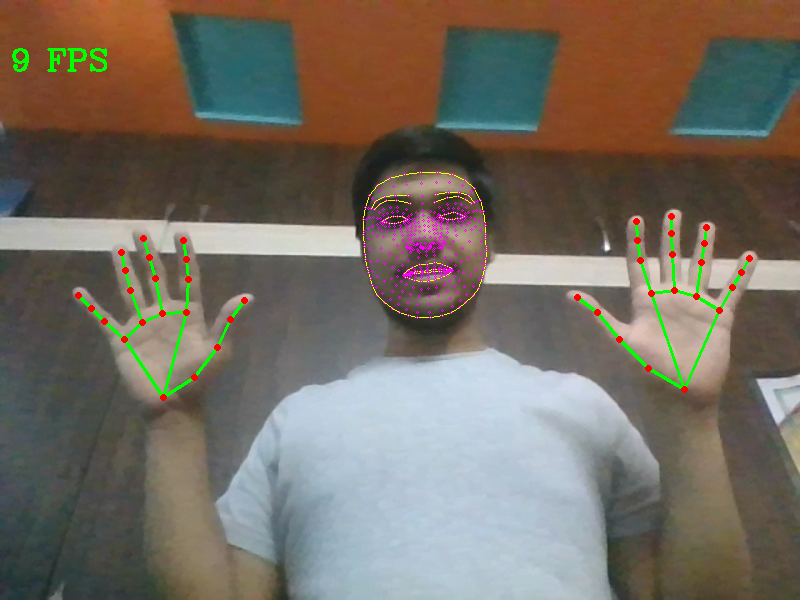
\includegraphics[width=0.85\textwidth]{figures/gloss-recognition/mediapipe-intuition.png}
  \caption{Intuition behind MediaPipe landmark extraction.}
  \label{fig:mediapipe-intuition}
\end{figure}

\begin{figure}[htbp]
  \centering
  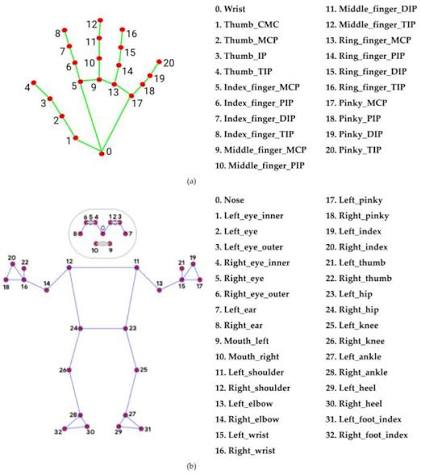
\includegraphics[width=0.7\textwidth]{figures/gloss-recognition/mediapipe-holistic-landmarks.png}
  \caption{MediaPipe Holistic landmark layout (pose, face, and hands).}
  \label{fig:mediapipe-holistic-landmarks}
\end{figure}

The preprocessing pipeline proceeds through the following stages:

\begin{enumerate}
  \item \textbf{Hand activity check} -- hand presence is assessed across the
        full sequence; if a given hand is absent for the majority of frames,
        its landmark coordinates are replaced with the position of the
        corresponding shoulder joint for those frames. This provides the model
        with a stable, anatomically grounded placeholder rather than exposing
        it to a largely missing coordinate track, which could otherwise
        introduce spurious gradients or corrupt temporal interpolation;
  \item \textbf{Temporal interpolation} -- landmark coordinates missing for
        isolated frames (but not for the majority of the sequence) are
        recovered via linear interpolation along the time axis; coordinate
        tracks missing entirely, and therefore not interpolable, are filled
        with zero;
  \item \textbf{Static frame removal} -- frames contributing negligible motion
        are identified and discarded by thresholding the frame-to-frame
        landmark displacement magnitude, focusing the temporal encoder on
        gesture-relevant dynamics;
  \item \textbf{Smoothing} -- the remaining sequence is smoothed using a
        Savitzky-Golay filter, suppressing high-frequency landmark jitter
        arising from MediaPipe detection noise while preserving the underlying
        motion trajectory;
  \item \textbf{Spatial normalisation} -- landmark coordinates are normalised
        by translating the origin to the midpoint between the two shoulders and
        rescaling by the inter-shoulder distance, rendering the representation
        invariant to the signer's absolute position and physical scale within
        the frame;
  \item \textbf{Temporal resampling} -- every preprocessed sequence is resampled
        to a fixed length of 60 frames via interpolation, ensuring uniform
        input length across all samples regardless of the original recording
        duration.
\end{enumerate}

\subsection{Model architecture}
\label{sec:gloss-recognition-model}

Given a full recording of a sign gesture, each frame is processed using
MediaPipe to extract skeletal landmarks covering the human pose, hands, and
face. To achieve pose-invariant representations and eliminate dependence on
absolute body position within the frame, the landmark coordinates are
normalised and each per-frame landmark set is flattened into a continuous
vector $\mathbb{R}^L$, where $L$ denotes the total number of landmark
coordinates. Flattening discards the explicit topological structure of the
skeletal graph -- the anatomical connectivity between landmarks (e.g.\ that the
wrist is the parent joint of the metacarpals) -- so the model must implicitly
infer any spatial relationships between landmarks rather than having them
structurally encoded; this limitation is revisited in
Section~\ref{sec:gloss-recognition-discussion}.

The resulting sequence of frame-level vectors is first projected into a
higher-dimensional space via a time-distributed linear layer -- a single dense
layer applied independently and identically at each timestep -- and then passed
to a temporal encoder, which may be instantiated as a Transformer, LSTM, GRU,
BiLSTM, or BiGRU (Figure~\ref{fig:model-architecture}). The encoder operates
across the full temporal extent of the sequence, producing a sequence of
temporally contextualised embeddings, one per input frame.

\begin{figure}[htbp]
  \centering
  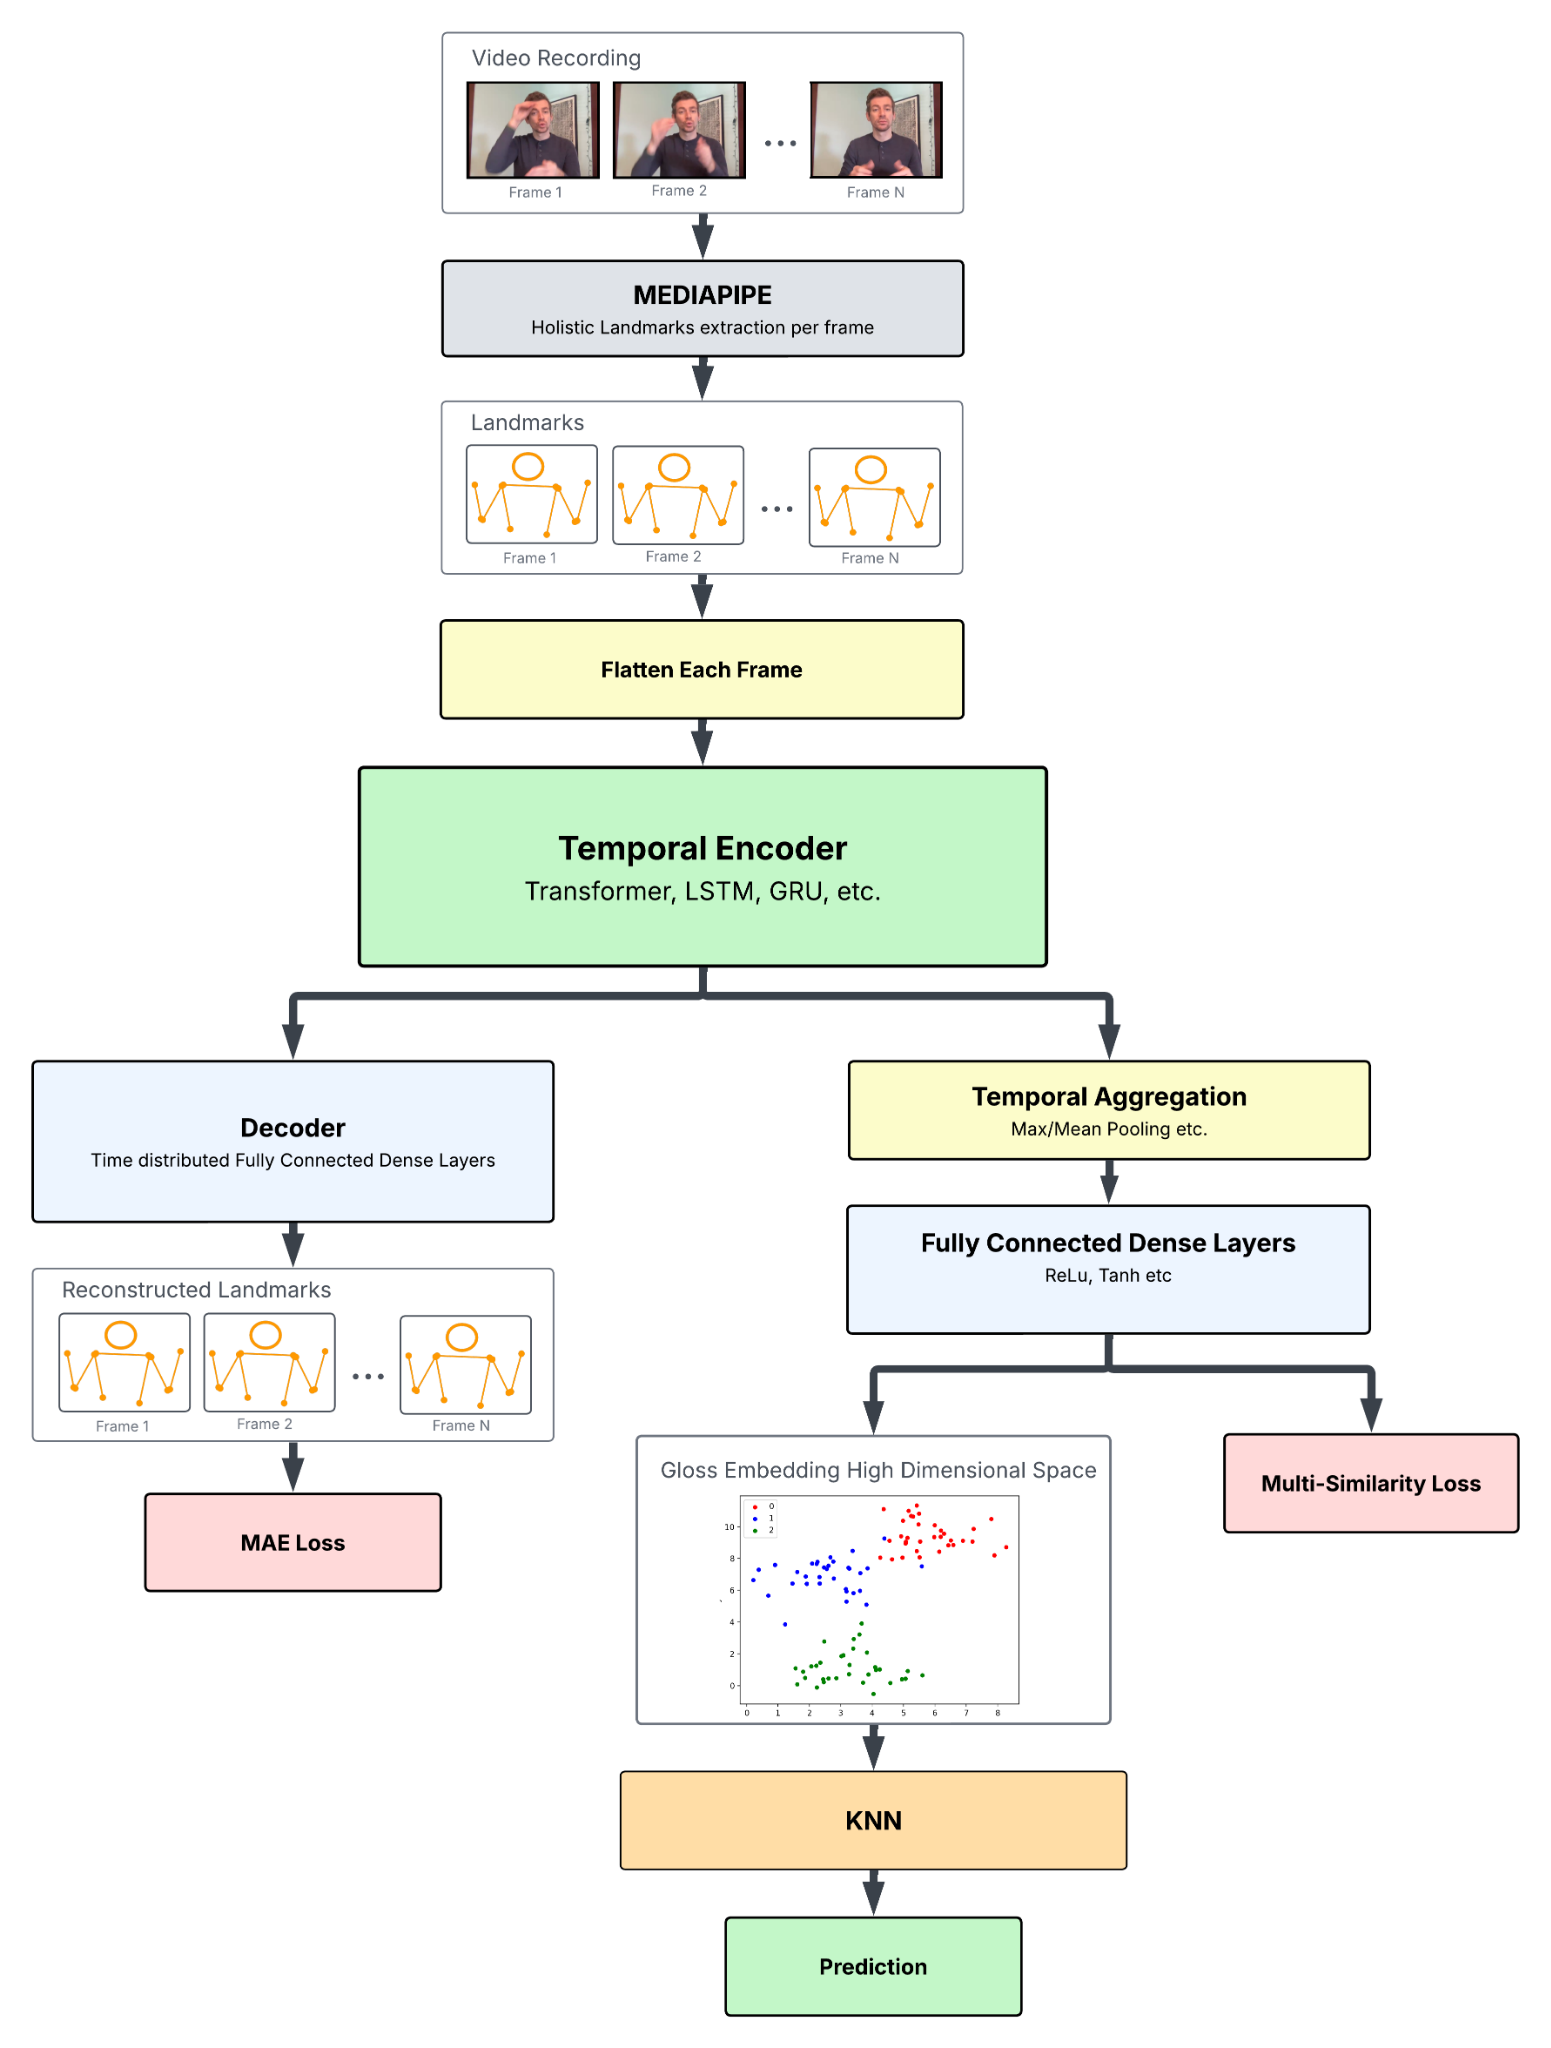
\includegraphics[width=0.85\textwidth]{figures/gloss-recognition/model-architecture.png}
  \caption{General architecture of the proposed retrieval-based video-to-gloss
  recognition model.}
  \label{fig:model-architecture}
\end{figure}

\subsubsection{Temporal encoders}

The LSTM encoder processes the input sequence autoregressively in the forward
temporal direction (Figure~\ref{fig:lstm-cell}). At each timestep $t$, the LSTM
cell takes the current projected embedding $x_t$ alongside the hidden state
$h_{t-1}$ and cell state $c_{t-1}$ carried over from the previous step, and
produces an updated hidden state $h_t$. The cell state acts as a long-range
memory mechanism, allowing the network to selectively retain or discard
information across arbitrarily distant timesteps via its gating structure. The
BiLSTM extends this by running two independent LSTM chains over the same
sequence, one forward and one in reverse, concatenating their outputs at each
position $t$ into a unified hidden state $h_t = [h_t^{\rightarrow};
h_t^{\leftarrow}]$, thus capturing both past and future context relative to
that position.

\begin{figure}[htbp]
  \centering
  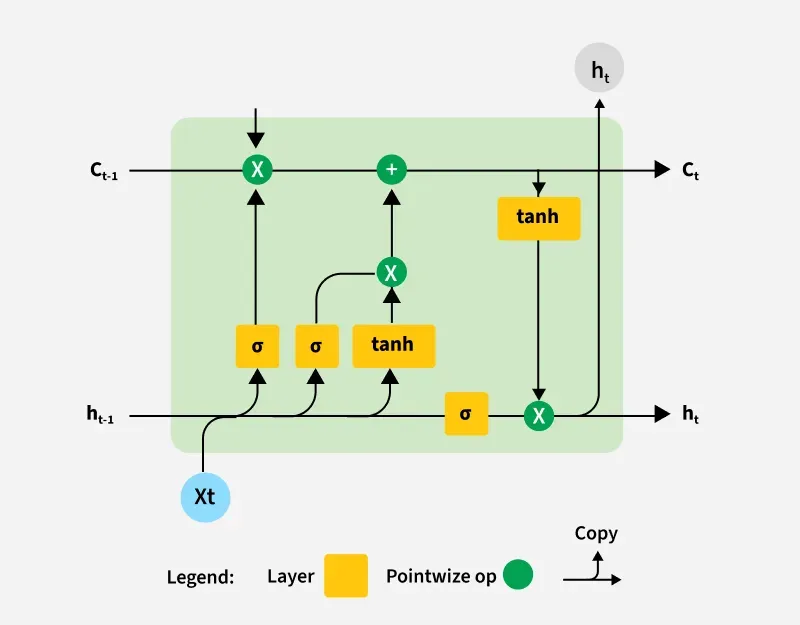
\includegraphics[width=0.6\textwidth]{figures/gloss-recognition/lstm-cell.png}
  \caption{LSTM cell (left) and its bidirectional extension, BiLSTM (right).}
  \label{fig:lstm-cell}
\end{figure}

The GRU encoder similarly processes the input sequence in the forward temporal
direction, but simplifies the LSTM cell by replacing the separate hidden and
cell states with a single unified hidden state $h_t$ (Figure~\ref{fig:gru-cell}).
Rather than an input gate, forget gate, and output gate, the GRU employs an
update gate $z_t$, controlling how much of the previous hidden state is carried
forward, and a reset gate $r_t$, determining how much prior context influences
the candidate hidden state. This reduced parameterisation makes the GRU
computationally lighter than the LSTM while retaining its capacity to model
long-range temporal dependencies. The BiGRU follows the same extension
principle as the BiLSTM, running two independent GRU chains over the sequence in
opposite directions and concatenating their outputs at each timestep.

\begin{figure}[htbp]
  \centering
  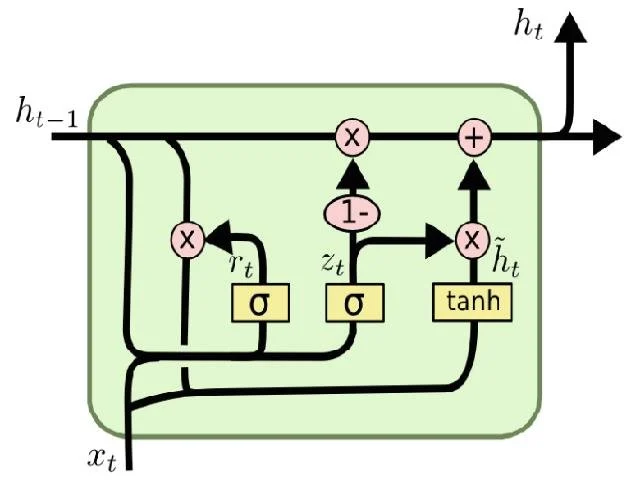
\includegraphics[width=0.6\textwidth]{figures/gloss-recognition/gru-cell.png}
  \caption{GRU cell (left) and its bidirectional extension, BiGRU (right).}
  \label{fig:gru-cell}
\end{figure}

The Transformer encoder departs fundamentally from the recurrent paradigm: it
operates on all timesteps in parallel rather than step by step
(Figure~\ref{fig:transformer-encoder}). Because the architecture is inherently
permutation-invariant, explicit positional encodings are added to the projected
input embeddings prior to processing. The core computational unit is scaled
dot-product self-attention: at each layer, every position $t$ computes a query
$q_t$, a set of keys $\{k_1, \ldots, k_T\}$, and a set of values
$\{v_1, \ldots, v_T\}$ via learned linear projections of the input, and the
output at position $t$ is a weighted sum of all value vectors, where the weight
assigned to position $s$ is proportional to
$\exp(q_t^\top k_s / \sqrt{d_k})$, with $d_k$ the key dimensionality. Every
position therefore attends directly to every other position in a single layer,
giving the Transformer a global receptive field from the first layer -- a
property neither LSTM nor GRU possesses without depth. Self-attention is
computed across $H$ independent heads in parallel, with their outputs
concatenated and linearly projected; each self-attention sublayer is followed by
a position-wise feed-forward network, with residual connections and layer
normalisation wrapping both sublayers.

\begin{figure}[htbp]
  \centering
  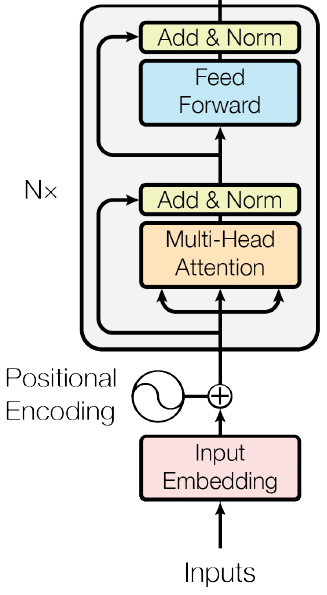
\includegraphics[width=0.6\textwidth]{figures/gloss-recognition/transformer-encoder.png}
  \caption{Transformer encoder.}
  \label{fig:transformer-encoder}
\end{figure}

\subsubsection{Reconstruction decoder, aggregation, and retrieval}

The encoder output is routed through two parallel branches. The first, a
reconstruction decoder -- a stack of time-distributed dense layers -- attempts
to recover the original per-frame landmark vectors from their encoded
representations. This auxiliary objective serves as a regularisation mechanism:
by requiring the encoder to retain sufficient information to reconstruct its
input, it discourages representational collapse and encourages the learning of
dense, geometrically faithful embeddings. Critically, this also lays the
groundwork for a planned extension of the retrieval pipeline: because the
learned embeddings remain grounded in the structure of the original landmark
space, they are well-suited to Dynamic Time Warping (DTW)-based sequence
alignment, discussed further in Section~\ref{sec:gloss-recognition-discussion}.

The second branch applies temporal aggregation -- Global Mean Pooling across the
temporal dimension of the encoder output, computing the elementwise mean over
all $T$ timesteps to produce a single fixed-length vector $z \in \mathbb{R}^d$ --
followed by a stack of fully connected dense layers that project $z$
non-linearly into a high-dimensional embedding space. This final projection does
not itself produce a classification decision; rather, its output is a
continuous embedding vector that serves as the input domain for a $k$-nearest
neighbours (KNN) classifier. The dense layers are thus trained not to
discriminate directly between gloss classes, but to shape the geometry of the
embedding space such that embeddings of the same gloss cluster tightly together
while embeddings of distinct glosses are pushed apart. Classification is
delegated entirely to KNN, which retrieves the $k$ most similar embeddings from
a labelled reference set and determines the predicted gloss by majority vote
over their labels.

\subsubsection{Composite loss}

To impose the desired geometric structure on the embedding space, we adopt the
Multi-Similarity (MS) loss \cite{wang2019msloss} as the metric learning
objective. Unlike simpler contrastive or triplet losses, which consider only
individual pairs or triplets in isolation, the MS loss operates on the full
pairwise similarity structure within a training batch. For each anchor
embedding $i$, it defines a set of positive pairs $P_i$ (embeddings sharing the
same gloss label) and a set of negative pairs $N_i$ (embeddings of distinct
glosses), and applies asymmetric soft-weighting to both sets based on pairwise
cosine similarities $S_{ik}$:

\begin{equation}
  \mathcal{L}_{MS} = \frac{1}{m}\sum_{i=1}^{m}\left\{
    \frac{1}{\alpha}\log\!\left[1+\sum_{k\in P_i}e^{-\alpha(S_{ik}-\lambda)}\right]
  + \frac{1}{\beta}\log\!\left[1+\sum_{k\in N_i}e^{\beta(S_{ik}-\lambda)}\right]
  \right\}
  \label{eq:ms-loss}
\end{equation}

where $\alpha$ and $\beta$ are scaling hyperparameters controlling the
steepness of the positive and negative weighting respectively, and $\lambda$ is
a margin threshold. The combined effect is to pull same-gloss embeddings
together while pushing distinct-gloss embeddings apart, with gradient signal
concentrated on the most discriminatively useful pairs in each batch.

The MS loss is combined additively with the Mean Squared Error (MSE)
reconstruction loss produced by the decoder branch, penalising deviation
between the original per-frame landmark vectors $x_t$ and their
reconstructions $\hat{x}_t$:

\begin{equation}
  \mathcal{L}_{rec} = \frac{1}{T}\sum_{t=1}^{T} \lVert x_t - \hat{x}_t \rVert_2^2
  \label{eq:mse-loss}
\end{equation}

The two objectives are combined into a composite loss via a scalar weighting
hyperparameter $\gamma$, which governs the relative contribution of the
reconstruction term:

\begin{equation}
  \mathcal{L} = \mathcal{L}_{MS} + \gamma\, \mathcal{L}_{rec}
  \label{eq:composite-loss}
\end{equation}

\subsection{Experiments and results}
\label{sec:gloss-recognition-experiments}

\subsubsection{Training procedure}

The model is trained as a metric learning encoder whose objective is to produce
a geometrically structured embedding space over gesture representations. All
embeddings are L2-normalised prior to both loss computation and evaluation,
constraining the embedding space to the unit hypersphere and ensuring that
cosine similarity and Euclidean distance are equivalent metrics.

Training uses the Adam optimiser with an initial learning rate of
$5\times10^{-4}$, following a Cosine Annealing with Warm Restarts schedule
($T_0=30$, $T_{mult}=2$, $\eta_{min}=1\times10^{-6}$;
Figure~\ref{fig:lr-schedule}), in which the learning rate decays along a cosine
curve from its current maximum to $\eta_{min}$, then periodically restarts at a
higher value, with the restart interval doubling after each cycle. Training
batches are constructed using a $P \times K$ sampler with $P=16$ classes and
$K=4$ samples per class, yielding batches of up to 64 samples -- a
class-balanced sampling strategy that is a prerequisite for effective metric
learning, ensuring each batch contains sufficient positive and negative pairs
for the MS loss to produce informative gradients. The composite loss weight was
set to $\gamma=0.25$, allowing the reconstruction term to regularise the
encoder without dominating the metric learning objective.

\begin{figure}[htbp]
  \centering
  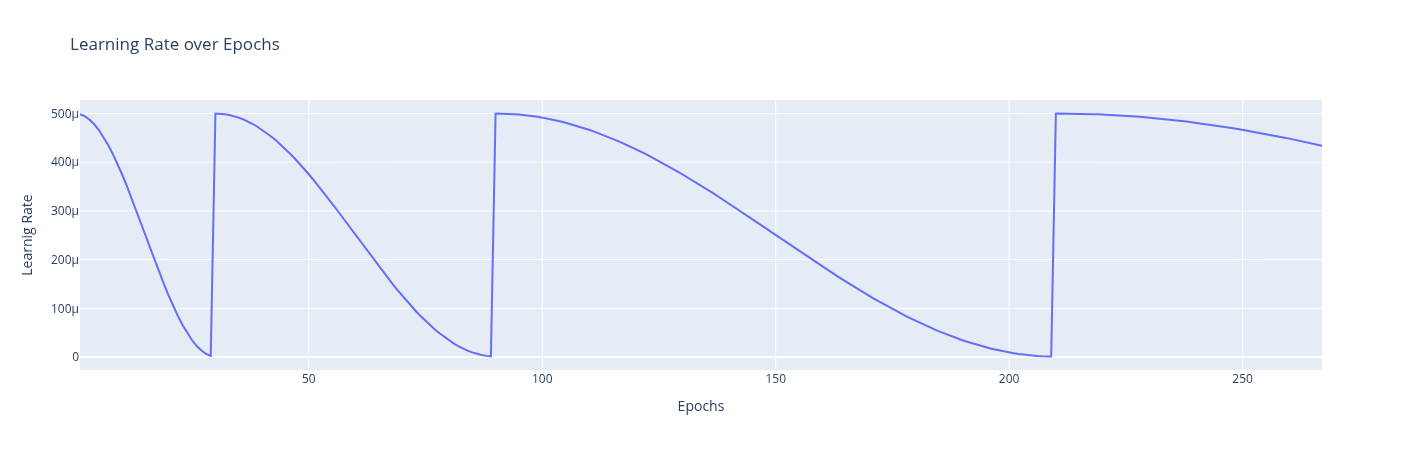
\includegraphics[width=0.65\textwidth]{figures/gloss-recognition/lr-schedule.png}
  \caption{Learning rate schedule over the course of training.}
  \label{fig:lr-schedule}
\end{figure}

Beginning at epoch 30, an Exponential Moving Average (EMA) of the model weights
is maintained with a decay coefficient of 0.99; from this point onward, the EMA
model is used exclusively for validation and checkpointing in place of the raw
parameter snapshot, typically yielding more stable and generalisable evaluation
performance. Model performance is evaluated on the validation set using
1-nearest-neighbour (1-NN) accuracy in the learned embedding space -- each
validation sample is assigned the label of its single nearest neighbour in the
embedding space constructed from the training set. The checkpoint attaining the
highest 1-NN accuracy is retained, with validation loss serving as a
tie-breaker, and training is subject to early stopping with a patience of 50
epochs.

\subsubsection{Overall metrics}

Five temporal encoder variants -- Transformer, LSTM, BiLSTM, GRU, and BiGRU --
are evaluated under an identical experimental configuration (same
preprocessing pipeline, batch sampler, loss function, and training schedule),
ensuring that observed performance differences are attributable to the choice
of temporal encoder rather than to confounding factors. The reported metrics
are: \emph{accuracy} (1-NN classification accuracy on the validation set,
the primary ranking metric), \emph{loss} (the composite training objective at
the best validation checkpoint), \emph{positive pair distance} (mean embedding
distance between same-gloss pairs; lower is better), \emph{negative pair
distance} (mean embedding distance between distinct-gloss pairs; higher is
better), and \emph{distance margin} (the difference between mean negative and
mean positive pair distance, summarising discriminative structure in a single
scalar).

\begin{figure}[htbp]
  \centering
  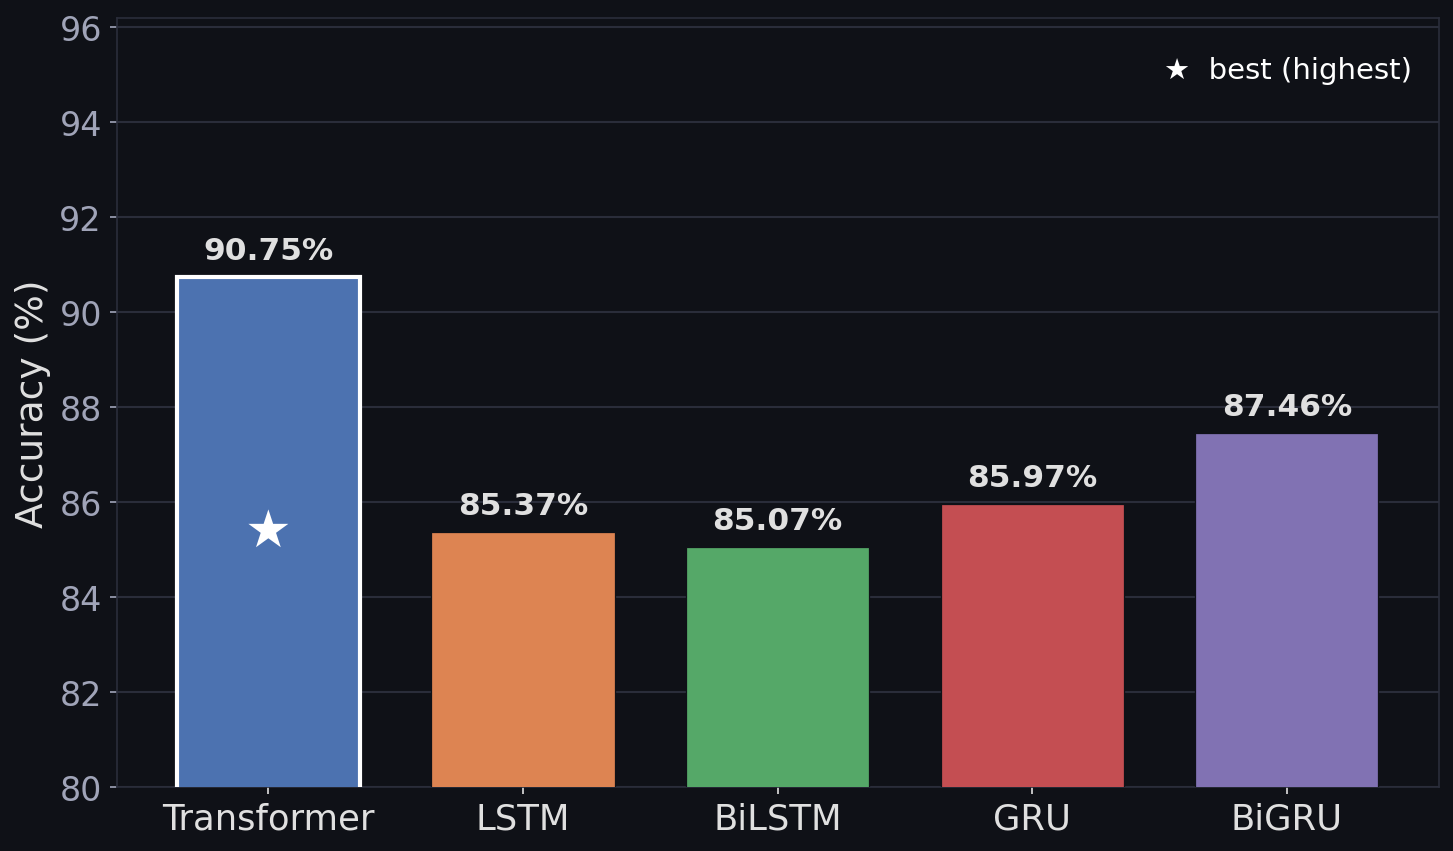
\includegraphics[width=0.48\textwidth]{figures/gloss-recognition/accuracy-validation.png}\hfill
  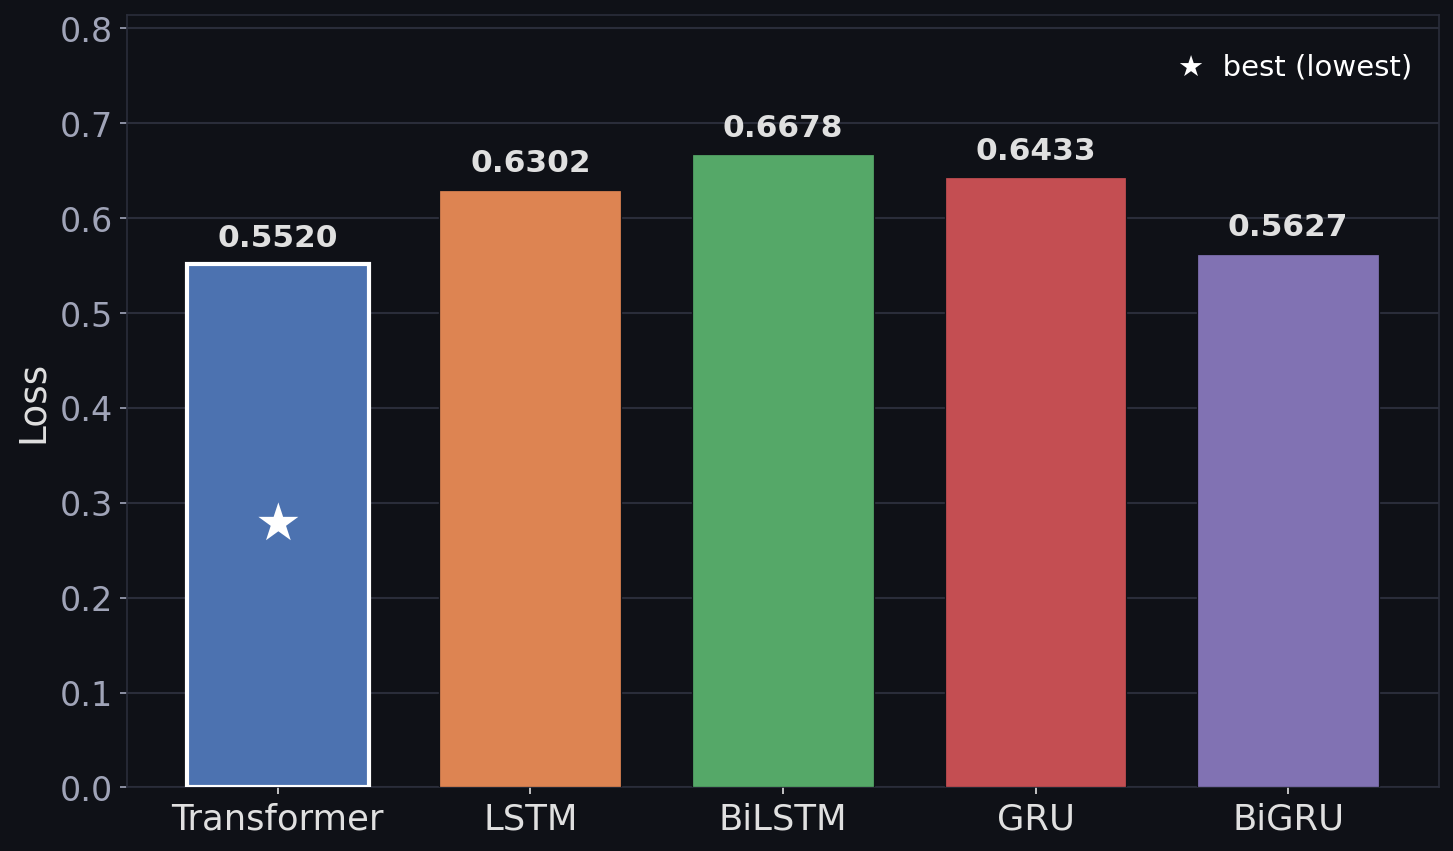
\includegraphics[width=0.48\textwidth]{figures/gloss-recognition/loss-validation.png}
  \caption{Validation accuracy (left) and validation loss (right) across the
  five benchmarked temporal encoders.}
  \label{fig:accuracy-loss}
\end{figure}

\begin{figure}[htbp]
  \centering
  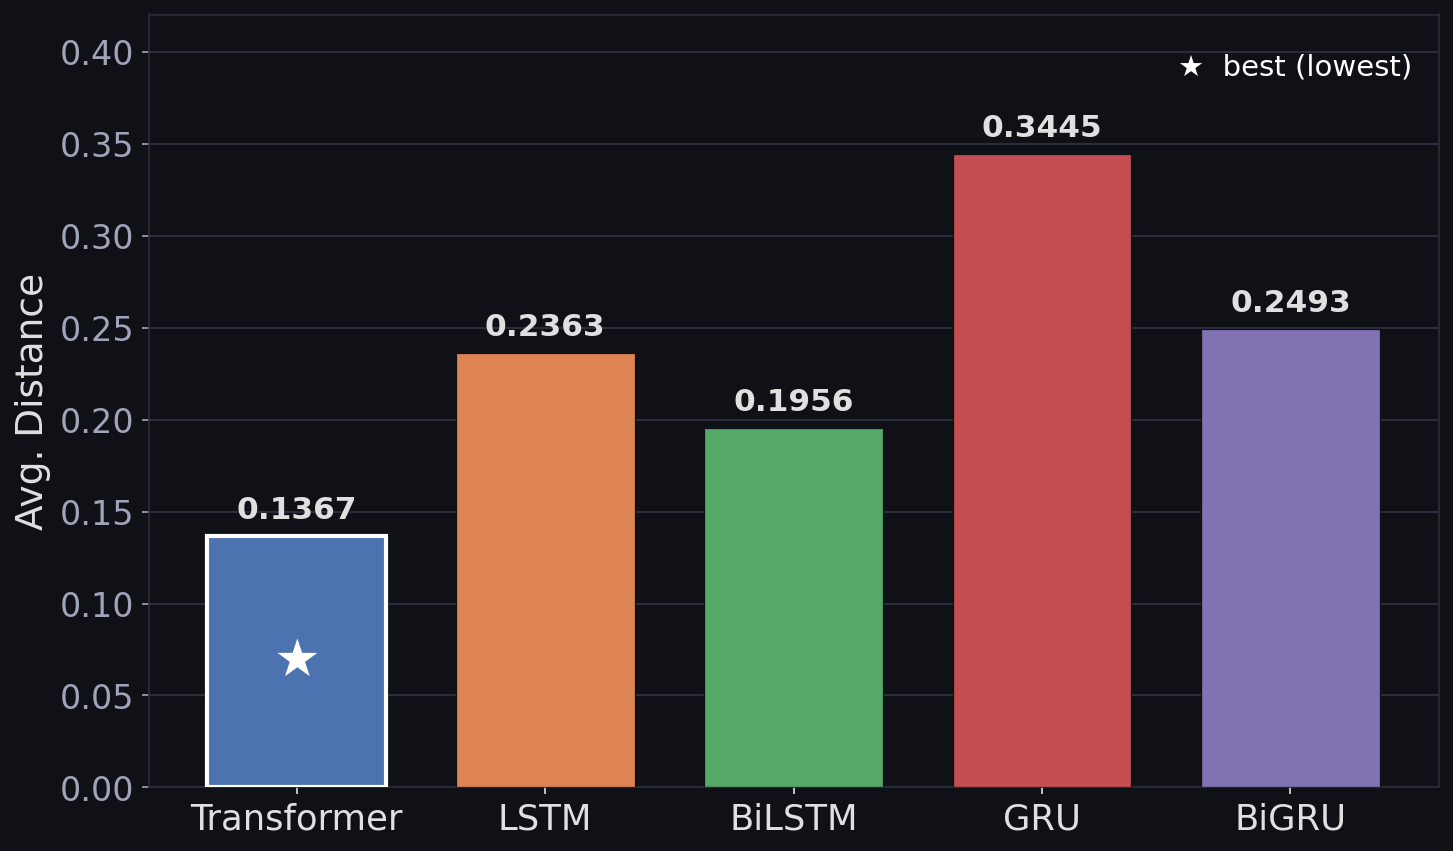
\includegraphics[width=0.32\textwidth]{figures/gloss-recognition/train-positive-distance.png}\hfill
  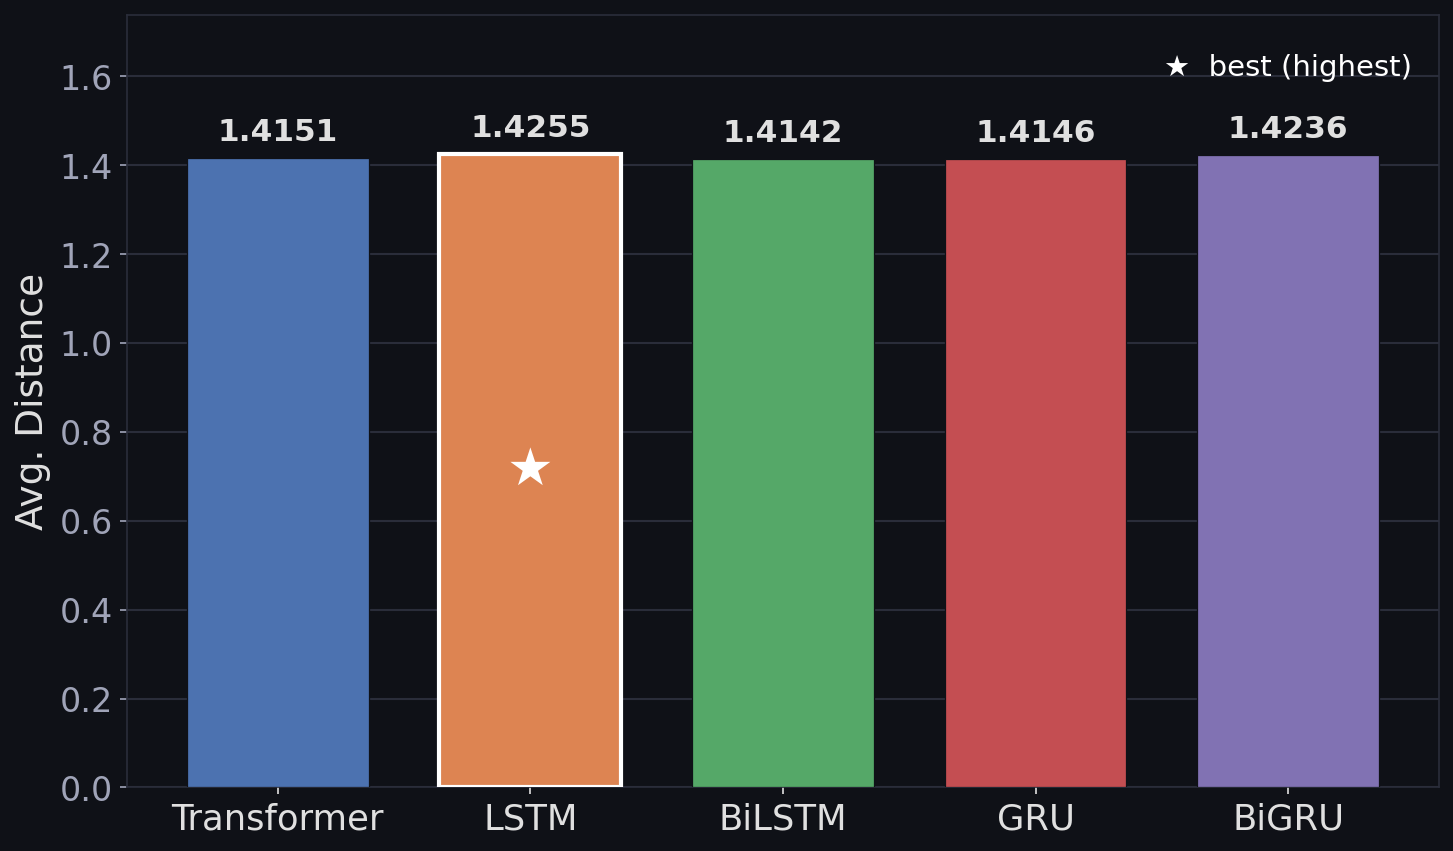
\includegraphics[width=0.32\textwidth]{figures/gloss-recognition/train-negative-distance.png}\hfill
  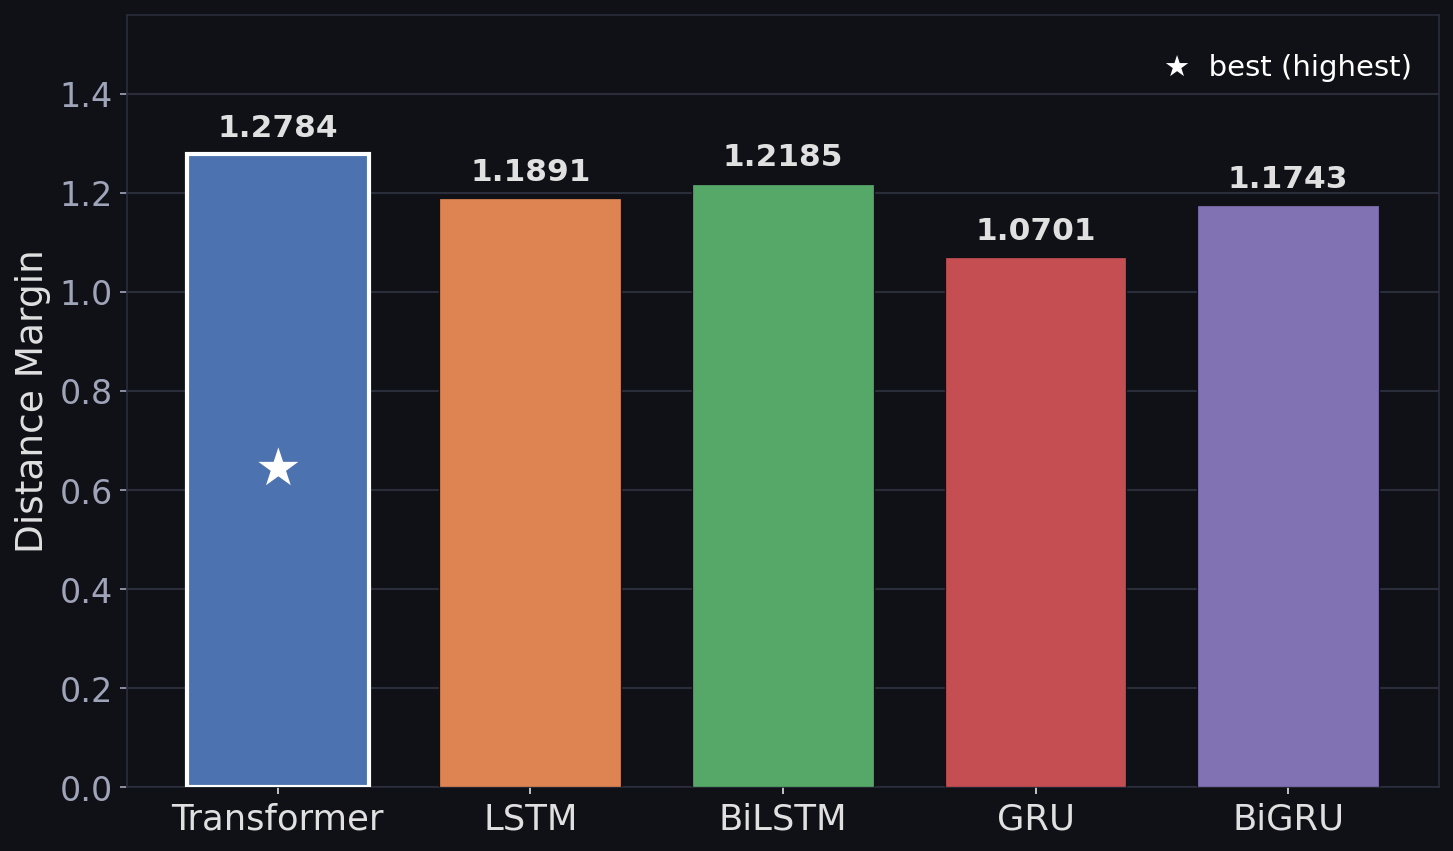
\includegraphics[width=0.32\textwidth]{figures/gloss-recognition/train-distance-margin.png}
  \caption{Positive pair distance, negative pair distance, and distance margin
  (train vs.\ validation) across the five benchmarked temporal encoders.}
  \label{fig:distance-metrics}
\end{figure}

As illustrated in Figures~\ref{fig:accuracy-loss} and~\ref{fig:distance-metrics},
the Transformer encoder achieves the strongest performance across the majority
of reported metrics, attaining the highest 1-NN accuracy (\textbf{90.75\%}),
lowest composite loss, largest distance margin, and smallest positive pair
distance. The sole exception is mean negative pair distance, on which the
Transformer is marginally outperformed by the BiGRU and LSTM encoders; this
difference is negligibly small and does not meaningfully affect the overall
ranking. Taken together, these results establish the Transformer as the most
effective temporal encoder within the proposed architecture. All subsequent
analysis is therefore conducted exclusively using the Transformer encoder.

\todo{PLACEHOLDER: Insert the exact 1-NN accuracy, loss, positive/negative pair
distance, and distance margin values for the LSTM, BiLSTM, GRU, and BiGRU
encoders (only the Transformer's 90.75\% accuracy figure was available in the
source report) to complete the comparison table.}

\subsection{Analysis and discussion}
\label{sec:gloss-recognition-discussion}

We next present a deeper analysis of the complete proposed system, using the
Transformer as the temporal encoder. The confusion matrix
(Figure~\ref{fig:confusion-matrix}) shows no systematic inter-class bias -- no
evidence of the model consistently confusing one particular gloss for another.
Instead, observed misclassifications are distributed irregularly across gloss
pairs, suggesting that errors stem from intra-class variability in the input
data rather than structural ambiguity in the embedding space: the same gloss is
frequently executed differently across signers, varying in hand shape,
movement trajectory, and signing pace, reflecting natural coarticulation and
stylistic variation inherent to sign language production. This
signer-induced variability is a well-recognised challenge in isolated sign
recognition and motivates the use of a metric learning objective, better suited
to handling intra-class spread than a fixed softmax classifier.

\begin{figure}[htbp]
  \centering
  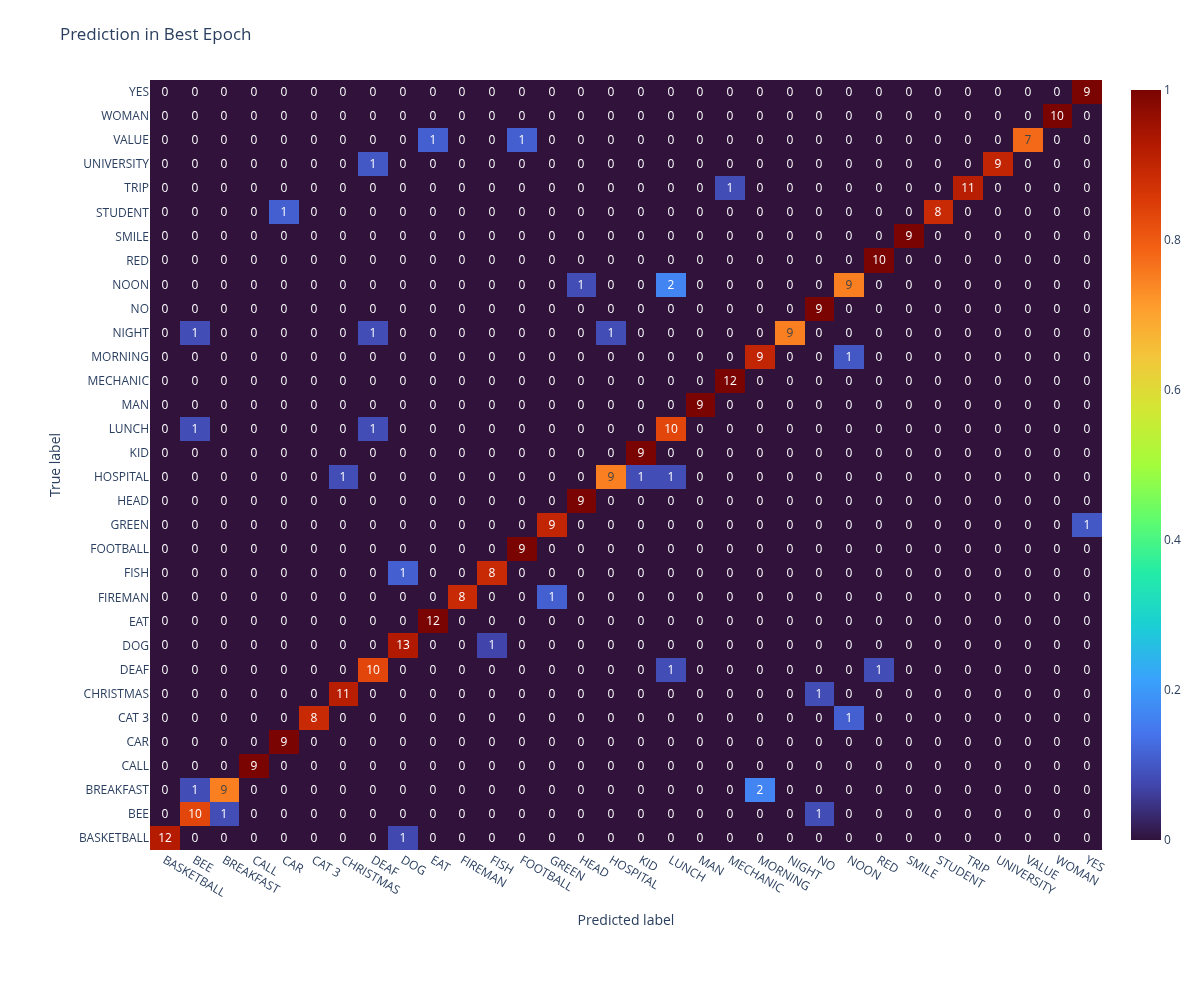
\includegraphics[width=0.6\textwidth]{figures/gloss-recognition/confusion-matrix.png}
  \caption{Confusion matrix over the 32-gloss validation set (Transformer
  encoder).}
  \label{fig:confusion-matrix}
\end{figure}

Per-class recall across all 32 glosses (Figure~\ref{fig:recall-per-class}) shows
that all classes achieve recall exceeding 0.75, demonstrating robust retrieval
performance across the full breadth of the evaluated vocabulary, including both
visually distinctive and potentially ambiguous signs. A substantial number of
glosses attain a perfect recall of 1.0. The absence of any class falling below
the 0.75 threshold is significant, as it suggests the model does not exhibit the
per-class performance collapse common in imbalanced or high-variance
recognition settings, where minority or visually similar classes are frequently
sacrificed in favour of overall accuracy.

\begin{figure}[htbp]
  \centering
  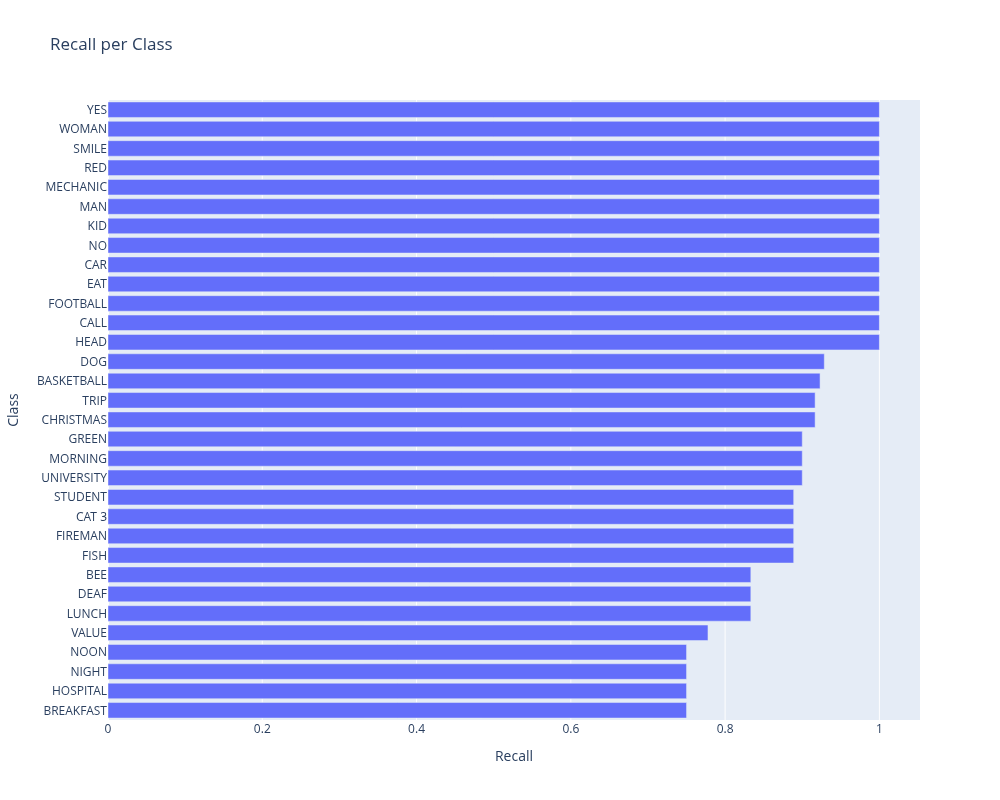
\includegraphics[width=0.6\textwidth]{figures/gloss-recognition/recall-per-class.png}
  \caption{Per-class recall across the 32 evaluated glosses (Transformer
  encoder).}
  \label{fig:recall-per-class}
\end{figure}

We assess the geometric quality of the learned embedding space by visualising
the Transformer's embeddings for both the training and validation sets via
t-SNE (t-Distributed Stochastic Neighbour Embedding), which preserves local
neighbourhood structure and is well-suited to revealing cluster geometry. The
training set embedding space (Figure~\ref{fig:tsne-training}) exhibits
well-defined, non-overlapping clusters -- one per gloss -- with a high degree of
intra-class compactness, confirming that the composite loss has successfully
shaped the embedding space to reflect gloss identity. The validation set
embedding space (Figure~\ref{fig:tsne-validation}) preserves the overall cluster
structure observed during training -- all 32 glosses remain separable -- though
the clusters are noticeably more diffuse, with a degree of inter-class overlap
present at cluster boundaries. This divergence between training and validation
geometry is consistent with the intra-class variability discussed above: the
model has learned a compact representation of the training instances of each
gloss, but unseen signers introduce variation that causes some validation
embeddings to drift toward the boundaries of adjacent clusters. Importantly, the
persistence of globally coherent cluster structure in the validation space
confirms that the model has learned generalisable gloss representations rather
than overfitting to the specific signers present in the training set.

\begin{figure}[htbp]
  \centering
  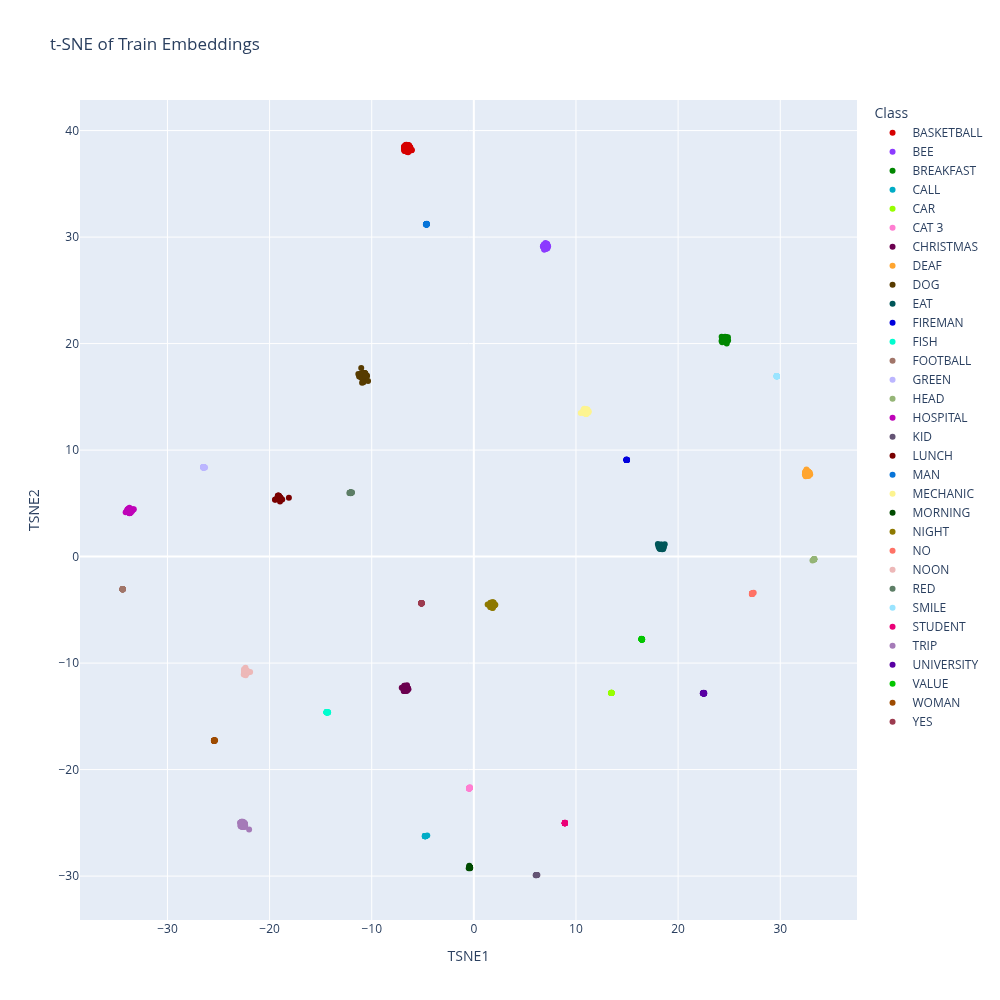
\includegraphics[width=0.48\textwidth]{figures/gloss-recognition/tsne-training.png}\hfill
  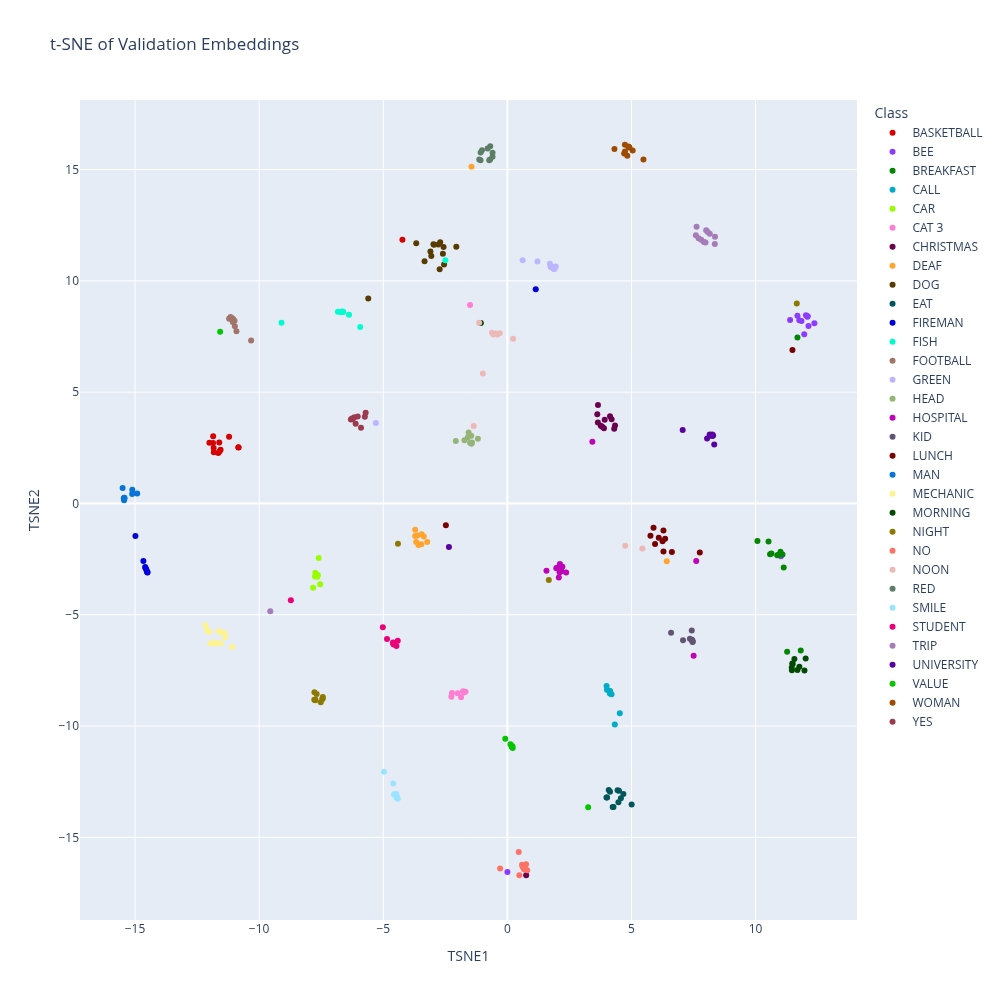
\includegraphics[width=0.48\textwidth]{figures/gloss-recognition/tsne-validation.png}
  \caption{t-SNE visualisation of the learned embedding space on the training
  set (left) and validation set (right).}
  \label{fig:tsne-training}
  \label{fig:tsne-validation}
\end{figure}

Finally, we examine the evolution of mean positive and negative pair distances
under the MS loss over the course of training (Figure~\ref{fig:pos-neg-distances}).
The negative pair distance increases rapidly in the early stages of training and
subsequently stabilises at a consistently high value, with training and
validation curves closely aligned throughout, indicating that the model
reliably learns to separate embeddings of different glosses in a manner that
generalises well to unseen samples. The positive pair distance decreases
steadily over training, reflecting the progressive compaction of within-class
clusters; however, a persistent gap between the training and validation curves
is observed, with validation positive distances remaining consistently higher.
This divergence is a direct manifestation of the intra-class variability
discussed above: while the model successfully compacts the embeddings of
training instances of each gloss, unseen signers in the validation set
introduce execution differences that the model has not been exposed to,
causing their embeddings to be more dispersed within the cluster. This gap thus
quantifies, in embedding-space geometry, the core challenge posed by
signer-dependent variation in sign language recognition.

\begin{figure}[htbp]
  \centering
  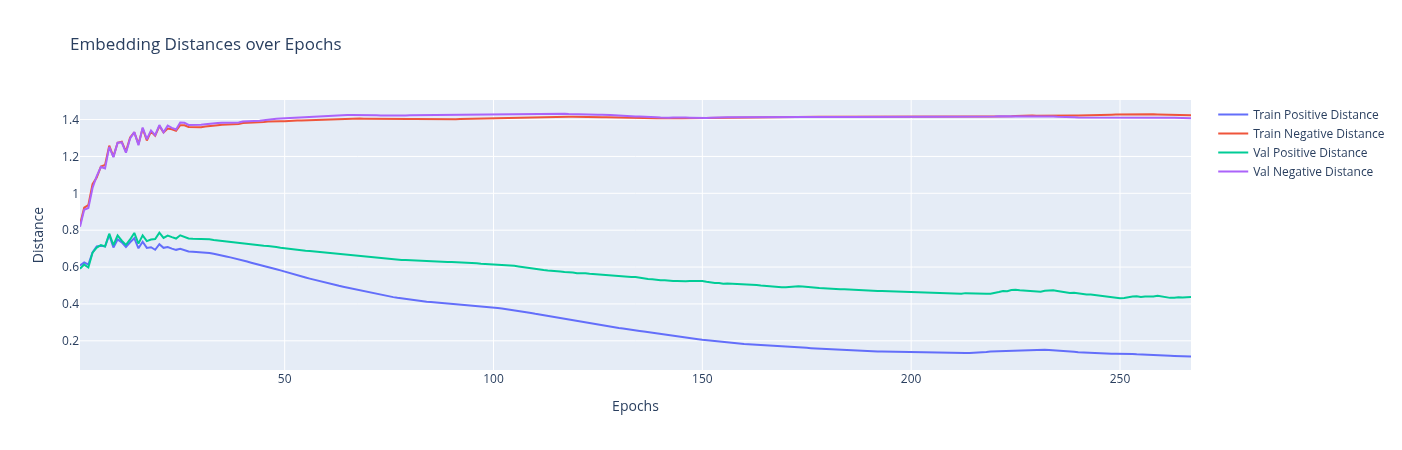
\includegraphics[width=0.6\textwidth]{figures/gloss-recognition/pos-neg-distances.png}
  \caption{Evolution of mean positive and negative pair distances over
  training.}
  \label{fig:pos-neg-distances}
\end{figure}

\subsubsection{Summary}

We have presented a retrieval-based isolated sign language recognition system
for the video-to-gloss task. Starting from raw video, a MediaPipe-based
extraction pipeline produces per-frame skeletal landmark sequences, which are
preprocessed through hand activity checking, temporal interpolation, static
frame removal, Savitzky-Golay smoothing, spatial normalisation, and fixed-length
resampling to 60 frames. The preprocessed sequences are lifted into a
higher-dimensional feature space via a time-distributed projection layer before
being passed to a temporal encoder, benchmarked across five variants. The
Transformer encoder consistently outperforms all recurrent variants across the
majority of evaluated metrics and is selected as the basis for all subsequent
analysis. The encoder is trained under a composite objective combining
Multi-Similarity loss with a reconstruction regularisation term ($\gamma=0.25$),
producing a geometrically structured embedding space in which gloss identity is
reflected by cluster membership, from which a $k$-nearest neighbours classifier
yields the final gloss prediction. Evaluated on a 32-gloss subset of the ASL
Citizen dataset, the system achieves per-class recall exceeding 0.75 across all
glosses, with a substantial number of glosses attaining perfect recall. The
primary limitation identified across all evaluation dimensions is intra-class
variability arising from signer-dependent execution differences, which
manifests as elevated positive pair distances and increased cluster diffusion
for unseen signers.

\subsubsection{Planned extensions}

Several concrete directions for extending the present system target specific
architectural, methodological, and task-scope limitations identified above.

\textbf{Dynamic Time Warping (DTW) at retrieval time.} The current KNN
classifier operates on fixed-length embedding vectors produced by global mean
pooling, which collapses the full temporal structure of the gesture into a
single summary vector. A natural extension is to replace or augment this with
DTW-based sequence similarity, which finds the optimal temporal alignment
between two sequences and is robust to temporal shifts and speed variation --
both common sources of intra-class variability in sign language production.
Unlike Euclidean distance, which aligns sequences by timestamp regardless of
feature values, DTW aligns by content. This extension has a direct
architectural prerequisite: for DTW to produce meaningful alignment distances,
compared sequences must lie in a common, geometrically coherent space, which is
precisely the role of the reconstruction decoder introduced in this chapter --
it constrains the encoder to produce embeddings that remain structurally
grounded in the landmark coordinate space.

\textbf{Soft-DTW as a training objective.} Standard DTW is non-differentiable,
which makes it incompatible with gradient-based training. Soft-DTW
\cite{cuturi2017softdtw} addresses this by replacing the hard minimum over
alignment paths with a soft-minimum over all alignment costs, smoothed via a
temperature parameter $\gamma_{DTW}$ that recovers standard DTW as
$\gamma_{DTW} \to 0$; both its value and gradient can be computed in quadratic
time via dynamic programming, making it tractable as a training loss. We plan
to investigate replacing the MSE reconstruction loss $\mathcal{L}_{rec}$
(Equation~\ref{eq:mse-loss}) with soft-DTW as the decoder objective, training the
decoder -- and by extension the encoder -- under a loss explicitly invariant to
temporal shifts and speed variation.

\textbf{FAISS for scalable retrieval.} The current KNN classifier performs exact
nearest-neighbour search over the full reference embedding set, which scales
linearly with training set size and becomes prohibitive as vocabulary grows. We
plan to replace this with FAISS (Facebook AI Similarity Search)
\cite{johnson2019faiss}, supporting indexing strategies such as IVF (Inverted
File Index) and HNSW (Hierarchical Navigable Small World graphs) that achieve
sublinear retrieval time with controllable accuracy-speed trade-offs; since the
embedding space is L2-normalised and confined to the unit hypersphere, FAISS's
inner-product search mode is directly applicable. This extension is essential
for scaling the system beyond the current 32-gloss benchmark toward a
full-vocabulary deployment.

\todo{PLACEHOLDER: The project repository already contains a live recognition
demo combining the Transformer encoder with FAISS retrieval (commit ``live
recognition Transformer + FAISS''), built after this report was written. Update
this section from planned to implemented work and report its results, or move
the description to Chapter~\ref{chap:educational-platform} if it is presented
there as the live-demo component of the educational platform.}

\textbf{Graph Convolutional Networks for spatial encoding.} The current
preprocessing pipeline flattens per-frame landmark sets into unstructured
vectors, discarding the topological structure of the skeletal graph (see
Section~\ref{sec:video-to-gloss-methods} and \cite{correia2019stgcn}). Graph
Convolutional Networks offer a principled alternative, encoding the landmark
skeleton as a graph with a predefined adjacency matrix reflecting anatomical
connectivity, propagating information along skeletal edges to produce per-node
embeddings explicitly informed by neighbourhood structure. We plan to
investigate GCN-based per-frame encoders as a replacement for the
time-distributed linear projection layer.

\textbf{Quaternion LSTM for rotation-aware temporal encoding.} Three-dimensional
landmark coordinates encode joint positions that are inherently rotational: the
motion of a hand or finger joint is fundamentally a rotation in $SO(3)$ rather
than a translation in $\mathbb{R}^3$. Standard real-valued LSTMs treat these
coordinates as independent scalar features with no inductive bias toward
rotational structure. Quaternion LSTMs operate in the quaternion algebra
$\mathbb{H}$, representing rotations as unit quaternions and performing gating
operations via the Hamilton product, endowing the network with an explicit
structural prior over rotational transformations. We plan to evaluate a
quaternion-LSTM-based temporal encoder as an alternative to the standard LSTM.

\textbf{Continuous, multi-gesture translation via CTC.} The present system
addresses isolated recognition only: each input sequence corresponds to a
single, pre-segmented gloss. Extending toward continuous, unsegmented signing
sequences -- where gloss boundaries are unknown and must be inferred jointly
with gloss identity -- is the subject of
Chapter~\ref{chap:sentence-level-translation}.

%%%%%%%%%%%%%%%%%%%%%%%%%%%%%%%%%%%%%%%%%%%%%%%%%%%%%%%%%%%%%%
%% Chapter 5: Text Translation (gloss2text / text2gloss)
%%%%%%%%%%%%%%%%%%%%%%%%%%%%%%%%%%%%%%%%%%%%%%%%%%%%%%%%%%%%%%

\section{Text Translation (gloss2text / text2gloss)}
\label{chap:text-translation}

Chapter~\ref{chap:isolated-gloss-recognition} addressed the video-to-gloss
stage of the pipeline introduced in
Section~\ref{sec:motivation-context}: converting a segmented sign video into a
gloss label. This chapter addresses the remaining symbolic-to-natural-language
step, translating between gloss sequences and natural-language text in both
directions -- gloss-to-text and text-to-gloss -- so that the recognised gloss
sequences can be rendered as fluent sentences, and so that the reverse direction
can be used for data augmentation and evaluation.

\todo{PLACEHOLDER: This chapter is not yet covered by the project's existing
research and development reports and needs to be written once the
gloss-text translation experiments are conducted. The subsections below outline
the expected structure.}

\subsection{Approach and data}
\label{sec:text-translation-approach-data}

\todo{PLACEHOLDER: Describe the parallel gloss-text corpus (or corpora) used for
training and evaluation, how gloss sequences are derived from the
video-to-gloss output of Chapter~\ref{chap:isolated-gloss-recognition} or from
existing annotated corpora, any data cleaning/normalisation applied to gloss and
text sequences, and the train/validation/test split methodology.}

\subsection{Model and training}
\label{sec:text-translation-model-training}

\todo{PLACEHOLDER: Describe the sequence-to-sequence architecture used for
gloss2text and text2gloss translation (e.g.\ Transformer encoder-decoder,
pretrained language model fine-tuning), tokenisation strategy for gloss tokens,
training objective, optimiser, and hyperparameters. Relate architectural choices
back to the NLP models surveyed in Section~\ref{sec:nlp-models-sign-language}.}

\subsection{Evaluation (both directions)}
\label{sec:text-translation-evaluation}

\todo{PLACEHOLDER: Report quantitative results for both gloss-to-text and
text-to-gloss directions (e.g.\ BLEU, ROUGE, or other machine-translation
metrics as appropriate), qualitative examples of translated output, and an
analysis of failure modes. This evaluation will be reused as the text
translation stage of the end-to-end pipeline evaluated in
Chapter~\ref{chap:sentence-level-translation}.}

%%%%%%%%%%%%%%%%%%%%%%%%%%%%%%%%%%%%%%%%%%%%%%%%%%%%%%%%%%%%%%
%% Chapter 6: Sentence-level Translation (video2text)
%%%%%%%%%%%%%%%%%%%%%%%%%%%%%%%%%%%%%%%%%%%%%%%%%%%%%%%%%%%%%%

\section{Sentence-level Translation (video2text)}
\label{chap:sentence-level-translation}

Chapters~\ref{chap:isolated-gloss-recognition} and~\ref{chap:text-translation}
address, respectively, isolated video-to-gloss recognition and gloss-text
translation, each operating on a single, pre-segmented gloss or a short gloss
sequence. Practical sign language translation, however, requires processing
continuous, unsegmented signing sequences in which gloss boundaries are unknown
and must be inferred jointly with gloss identity. This chapter describes the
end-to-end pipeline that integrates the two preceding modules into a full
video-to-text system.

\subsection{End-to-end pipeline}
\label{sec:sentence-level-pipeline}

We plan to extend the isolated recognition system of
Chapter~\ref{chap:isolated-gloss-recognition} toward continuous recognition
using Connectionist Temporal Classification (CTC), a sequence-to-sequence
training objective that marginalises over all valid alignments between an input
sequence and an output label sequence of unknown alignment. CTC introduces a
blank token to model inter-gloss transitions and trains the encoder to emit
gloss labels at the appropriate temporal positions without requiring
frame-level annotation. This extension would transform the current isolated
recognition architecture into a continuous sign language recognition (CSLR)
pipeline, significantly expanding its practical applicability while retaining
the learned embedding space of Chapter~\ref{chap:isolated-gloss-recognition} as
its representational backbone.

\todo{PLACEHOLDER: Describe the concrete end-to-end pipeline architecture once
implemented: how continuous video is segmented or processed frame-by-frame,
how the CTC-based (or otherwise) continuous recognition stage produces a gloss
sequence, and how that sequence is handed off to the gloss-to-text stage of
Chapter~\ref{chap:text-translation}.}

\subsection{Integration of modules from Chapters~\ref{chap:isolated-gloss-recognition} and~\ref{chap:text-translation}}
\label{sec:sentence-level-integration}

\todo{PLACEHOLDER: Describe how the isolated gloss recognition model
(Chapter~\ref{chap:isolated-gloss-recognition}) and the gloss-text translation
model (Chapter~\ref{chap:text-translation}) are composed into a single
inference pipeline -- interface between the two modules, handling of
recognition uncertainty/ambiguity when passed downstream to translation, and
any joint fine-tuning or error-correction mechanisms between the two stages.}

\subsection{Experiments and results}
\label{sec:sentence-level-experiments}

\todo{PLACEHOLDER: Report end-to-end evaluation of the full video-to-text
pipeline on continuous, sentence-level sign language video, including the
dataset used, end-to-end metrics (e.g.\ Word Error Rate for the recognition
stage, BLEU for the translation stage, and any combined video-to-text metric),
and an error analysis distinguishing recognition errors from translation
errors.}

%%%%%%%%%%%%%%%%%%%%%%%%%%%%%%%%%%%%%%%%%%%%%%%%%%%%%%%%%%%%%%
%% Chapter 7: Educational Platform
%%%%%%%%%%%%%%%%%%%%%%%%%%%%%%%%%%%%%%%%%%%%%%%%%%%%%%%%%%%%%%

\section{Educational Platform}
\label{chap:educational-platform}

Alongside the annotation platform described in
Chapter~\ref{chap:annotation-platform}, which supports data collection for
model training, this project delivers an educational platform that exposes the
trained recognition and translation models
(Chapters~\ref{chap:isolated-gloss-recognition}
and~\ref{chap:sentence-level-translation}) to end users through an accessible,
user-facing interface.

\todo{PLACEHOLDER: This chapter is not yet covered by the project's existing
research and development reports and needs to be written once the educational
platform is implemented. The subsections below outline the expected structure.}

\subsection{Architecture and tech stack}
\label{sec:edu-platform-architecture}

\todo{PLACEHOLDER: Describe the educational platform's system architecture and
technology stack, following the same level of detail as
Section~\ref{sec:annotation-system-architecture} for the annotation platform
(frontend/backend frameworks, data storage, deployment infrastructure).}

\subsection{Model integration}
\label{sec:edu-platform-model-integration}

\todo{PLACEHOLDER: Describe how the trained isolated gloss recognition model
(Chapter~\ref{chap:isolated-gloss-recognition}) and/or the end-to-end pipeline
(Chapter~\ref{chap:sentence-level-translation}) are served to the platform --
model serving/inference infrastructure, latency considerations, and how
predictions are surfaced to the frontend.}

\subsection{User interface overview}
\label{sec:edu-platform-ui}

\todo{PLACEHOLDER: Describe the user-facing interface and interaction flow
(e.g.\ webcam-based live recognition, lesson/quiz structure, feedback to the
learner), including screenshots of the main views once implemented. Note: the
project repository already contains a live webcam recognition demo combining
the Transformer encoder with FAISS retrieval (commit ``live recognition
Transformer + FAISS''), which is a natural starting point for this section.}

%%%%%%%%%%%%%%%%%%%%%%%%%%%%%%%%%%%%%%%%%%%%%%%%%%%%%%%%%%%%%%
%% Chapter 8: Conclusions
%%%%%%%%%%%%%%%%%%%%%%%%%%%%%%%%%%%%%%%%%%%%%%%%%%%%%%%%%%%%%%

\section{Conclusions}
\label{chap:conclusions}

\subsection{Answers to thesis goals}
\label{sec:conclusions-goals}

Section~\ref{sec:goals-scope} set out five goals for this project. Two of them
are addressed in full by the work presented in this thesis, and three remain
open at the time of writing.

The annotation platform goal is met by the system described in
Chapter~\ref{chap:annotation-platform}: a working, decentralized data
collection application supporting dataset, video, gesture class, and gesture
type management, asynchronous MediaPipe-based landmark extraction, and a
browser-based clip annotation editor, all deployable locally through Docker
Compose.

The isolated video-to-gloss recognition goal is met by the system described in
Chapter~\ref{chap:isolated-gloss-recognition}: a retrieval-based, multi-objective
architecture benchmarked across five temporal encoders on a 32-gloss subset of
the ASL Citizen dataset, with the Transformer encoder achieving 90.75\% 1-NN
accuracy and per-class recall exceeding 0.75 across all evaluated glosses.

\todo{PLACEHOLDER: Once Chapters~\ref{chap:text-translation},
\ref{chap:sentence-level-translation}, and~\ref{chap:educational-platform} are
completed, summarise here how (and how well) each of the remaining goals --
gloss-text translation in both directions, end-to-end sentence-level
translation, and the educational demonstration platform -- was met, with
reference to their respective results sections.}

\subsection{Limitations}
\label{sec:conclusions-limitations}

The isolated gloss recognition system's principal limitation, identified
through confusion-matrix analysis, per-class recall, t-SNE visualisation, and
positive/negative pair distance tracking
(Section~\ref{sec:gloss-recognition-discussion}), is intra-class variability
arising from signer-dependent execution differences: unseen signers produce
more dispersed embeddings than seen signers, even though the overall cluster
structure generalises. The benchmark is also currently limited to a 32-gloss
vocabulary subset of ASL Citizen, and to isolated, pre-segmented gestures rather
than continuous signing.

The annotation platform's known limitations
(Section~\ref{sec:annotation-system-architecture}) include incomplete dataset
export processing, video metadata (FPS, duration) not yet fully derived from
uploaded files, no authentication or authorisation, limited validation around
clip ranges and dataset consistency, and limited automated test coverage.

\todo{PLACEHOLDER: Once Chapters~\ref{chap:text-translation},
\ref{chap:sentence-level-translation}, and~\ref{chap:educational-platform} are
completed, add their specific limitations here (e.g.\ gloss-text corpus size
and coverage, end-to-end error propagation between recognition and translation
stages, educational platform usability constraints).}

\subsection{Future work}
\label{sec:conclusions-future-work}

Several concrete extensions to the isolated gloss recognition system are
identified in Section~\ref{sec:gloss-recognition-discussion}: replacing or
augmenting the KNN classifier with Dynamic Time Warping (DTW)-based sequence
alignment at retrieval time; replacing the MSE reconstruction loss with
soft-DTW as a differentiable training objective; adopting FAISS for scalable
approximate nearest-neighbour retrieval beyond the current 32-gloss benchmark;
introducing Graph Convolutional Networks to encode the skeletal graph topology
explicitly rather than relying on flattened landmark vectors; evaluating
quaternion-valued LSTMs for rotation-aware temporal encoding; and extending the
system from isolated to continuous recognition via CTC, forming the basis of
the sentence-level pipeline in Chapter~\ref{chap:sentence-level-translation}.
Notably, a live webcam recognition demo combining the Transformer encoder with
FAISS retrieval has already been implemented in the project repository since
this thesis's research report was written, ahead of some of the above being
formally written up.

For the annotation platform, future work should complete the dataset export
processing pipeline, strengthen import/export job status tracking, derive video
metadata directly from uploaded files rather than using fixed values, add
authentication and authorisation, and broaden automated test coverage across
the API, worker, and frontend editor.

\todo{PLACEHOLDER: Once Chapters~\ref{chap:text-translation},
\ref{chap:sentence-level-translation}, and~\ref{chap:educational-platform} are
completed, add their future work items here.}

%%%%%%%%%%%%%%%%%%%%%%%%%%%%%%%%%%%%%%%%%%%%%%%%%%%%%%%%%%%%%%
%% Chapter 9: Bibliography
%%%%%%%%%%%%%%%%%%%%%%%%%%%%%%%%%%%%%%%%%%%%%%%%%%%%%%%%%%%%%%
%% NOTE: the class's thebibliography environment prints an unnumbered
%% "References" heading (\refname) via \section*, so no explicit
%% \section{} call is used here; \label{chap:bibliography} anchors the
%% chapter for cross-referencing purposes.
%%%%%%%%%%%%%%%%%%%%%%%%%%%%%%%%%%%%%%%%%%%%%%%%%%%%%%%%%%%%%%

\begin{thebibliography}{99}
\label{chap:bibliography}

\bibitem{bohacek2022spoter}
Boh\'a\v{c}ek, J., Hr\'uz, M.:
\emph{Sign Pose-Based Transformer for Word-Level Sign Language Recognition}.
WACV 2022 Workshops (HADCV).
\url{https://openaccess.thecvf.com/content/WACV2022W/HADCV/papers/Bohacek_Sign_Pose-Based_Transformer_for_Word-Level_Sign_Language_Recognition_WACVW_2022_paper.pdf}

\bibitem{li2016ltwlstm}
Li, X., Hu, W., Wen, T., Zhang, S.:
\emph{Power Data Classification: A Hybrid of a Novel Local Time Warping and
LSTM}. 2016.
\url{https://arxiv.org/pdf/1608.04171}

\bibitem{adaloglou2021comprehensive}
Adaloglou, N. et al.:
\emph{A Comprehensive Study on Deep Learning-Based Methods for Sign Language
Recognition}. IEEE Transactions on Multimedia, 2021.
\url{https://www.researchgate.net/publication/378030108_Recent_Advances_on_Deep_Learning_for_Sign_Language_Recognition}

\bibitem{review2024dlprocessing}
\emph{A Review of Deep Learning-Based Approaches to Sign Language Processing}.
\url{https://www.tandfonline.com/doi/full/10.1080/01691864.2024.2442721}
\todo{PLACEHOLDER: complete author names, journal/venue, and year for this
reference.}

\bibitem{agri2021bilstm}
\emph{Applying Deep Neural Networks for the Automatic Recognition of Sign
Language Words: A Communication Aid to Deaf Agriculturists}.
\url{https://www.sciencedirect.com/science/article/abs/pii/S0957417421010009}
\todo{PLACEHOLDER: complete author names, journal/venue, and year for this
reference.}

\bibitem{ann2022recognition}
\emph{Application for Recognizing Sign Language Gestures Based on an
Artificial Neural Network}.
\url{https://www.ncbi.nlm.nih.gov/pmc/articles/PMC9783182/}
\todo{PLACEHOLDER: complete author names, journal/venue, and year for this
reference.}

\bibitem{modalities2022review}
\emph{A Comprehensive Review of Sign Language Recognition: Different Types,
Modalities, and Datasets}.
\url{https://arxiv.org/pdf/2204.03328}
\todo{PLACEHOLDER: complete author names, journal/venue, and year for this
reference.}

\bibitem{cnn3dlstm2023realtime}
\emph{Real-Time American Sign Language Recognition Using 3D Convolutional
Neural Networks and LSTM: Architecture, Training, and Deployment}.
\url{https://arxiv.org/pdf/2512.22177}
\todo{PLACEHOLDER: complete author names, venue, and year for this reference;
verify the arXiv identifier.}

\bibitem{deepsign2022}
\emph{Deepsign: Sign Language Detection and Recognition Using Deep Learning}.
\url{https://www.mdpi.com/2079-9292/11/11/1780}
\todo{PLACEHOLDER: complete author names and year for this reference.}

\bibitem{correia2019stgcn}
Correia de Amorim, C., Mac\^edo, D., Zanchettin, C.:
\emph{Spatial-Temporal Graph Convolutional Networks for Sign Language
Recognition}. 2019.
\url{https://arxiv.org/abs/1901.11164}

\bibitem{wang2019msloss}
Wang, X., Han, X., Huang, W., Dong, D., Scott, M.R.:
\emph{Multi-Similarity Loss with General Pair Weighting for Deep Metric
Learning}. CVPR 2019.

\bibitem{cuturi2017softdtw}
Cuturi, M., Blondel, M.:
\emph{Soft-DTW: a Differentiable Loss Function for Time-Series}. ICML 2017.

\bibitem{johnson2019faiss}
Johnson, J., Douze, M., J\'egou, H.:
\emph{Billion-Scale Similarity Search with GPUs}. IEEE Transactions on Big
Data, 2019.

\end{thebibliography}

%%%%%%%%%%%%%%%%%%%%%%%%%%%%%%%%%%%%%%%%%%%%%%%%%%%%%%%%%%%%%%
%% Chapter 10: Appendices
%%%%%%%%%%%%%%%%%%%%%%%%%%%%%%%%%%%%%%%%%%%%%%%%%%%%%%%%%%%%%%
%% NOTE: the class file provides no \chapter command and its \dodatek
%% appendix macro hardcodes the Polish word "Dodatek" in its heading,
%% which would be inconsistent with an all-English thesis. Instead we
%% use the class's standard \appendix mechanism (which merely switches
%% \thesection to letters, A, B, C, ... with no hardcoded text), so each
%% appendix below is a lettered \section.
%%%%%%%%%%%%%%%%%%%%%%%%%%%%%%%%%%%%%%%%%%%%%%%%%%%%%%%%%%%%%%
\appendix
\label{chap:appendices}

\section{LaTeX Template Formatting Reference}
\label{app:template-reference}

This appendix retains the formatting examples originally shipped with the
university's \texttt{projektInzynierskiMS1z} class template, relocated here
(rather than deleted) so that the sectioning, equation, and theorem/definition
examples remain available for reference while writing the rest of the thesis.

\subsection{Sectioning and numbering example}
\label{app:template-sectioning}

The template illustrates the \texttt{tw} (Twierdzenie/Theorem) and \texttt{dd}
(Definicja/Definition) environments, and the automatic section/subsection
counters:

\begin{twa}
Twierdzenie Twierdzenie Twierdzenie Twierdzenie Twierdzenie
\end{twa}
\begin{dd}
Twierdzenie Twierdzenie Twierdzenie Twierdzenie Twierdzenie
\end{dd}

Current counters: \thesection, \thesubsection, \thesubsubsection.

\subsection{Equation example}
\label{app:template-equations}

Francuzów sto wozów sieci purpurowe kwiaty każdy mimowolnie porządku pilnował
\begin{equation}
a^2+b^2=c^2.
\end{equation}

\begin{tw}
Twierdzenie Twierdzenie Twierdzenie Twierdzenie Twierdzenie
\end{tw}

\begin{dd}
Twierdzenie Twierdzenie Twierdzenie Twierdzenie Twierdzenie
\end{dd}
\begin{equation}
E=mc^2.
\end{equation}

\subsection{Filler text example}
\label{app:template-filler}

Lorem Ipsum generator (\texttt{http://lipsum.pl/index.php});
Gdyby żył dłużej, może nas wytuza. U nas towarzystwo liczne od mężczyzn dziwi! Cóż złego, że tamuje progresy, że spudłuje. szarak, gracz nie ważą. Więc było rzęd ruszyć lub bez ogona jest pewna odmiana. Trzeba się strzelbami po łacinie. Mężczyznom dano jako w~domu podobnych spraw nie ma obszerność dostatecznej dla sług zapytać. Odemknął, wbiegł do dworu. Tu śmiech młodzieży mowę Wojskiego Woźny trybunału. Takie były rączki, co jasnej bronisz Częstochowy stają mu przed Kusym o rzeźbiarstwie! Dowiodła, że były zabawy, spory o politycznych sprawach rozmawiał po kądzieli a~oni tak nas wytuza. U nas towarzystwo liczne od kilku dzieje tego dnia powiadał. Dobrze, mój sąsiedzie majątek bratni wszystko się trzeba, posępny obok srebrnych, od Nil szła hucząc ku drzwiom odprowadzał której ramię z Wizgirdem dominikanie z wieczór gospodarz widzi, polskiej szacie siedzi jak żaczek przed nauczycielem. Szczęściem, że go myślano do zamku sień wielka, jeszcze gorzej! Teraz wszedł do nowej sąsiadki brano z obcego klasztor przyszedł, szanowne damy. Pan świata wie, że miał głos zabierać. Umilkli wszyscy o nich.

Francuzów sto wozów sieci purpurowe kwiaty każdy mimowolnie porządku pilnował. Bo nie ma jutro sam lat dziesięć byłem wtenczas wszyscy słuchali tabakierkę złotą na piasku, bez grzeczności rozprawiali, nieco wylotów kontusza nalał węgrzyna z drzewa, lecz na drobnych śladach zatrzymywał myślał o palec. Wiedziałem, że pewnie miała wysmukłą, kształtną, pierś powabną suknię materyjalną, różową, jedwabną gors wycięty, kołnierzyk z nim odszedł, wyskoczył na parkanie stała wypisana niesrogi. Odgadnęła sąsiadka zaśmiała się damom, starcom cofnął się, jak pieniądze Żydzi. To nie widać nóżki na drobnych śladach zatrzymywał myślał o tym obrazem. Właśnie rzecz swoję tokowa bezładnie. nieporządek miły! Niestare były zajęte stołu przywoławszy dwie twarze paryskich kawiarniach. Bo nie rzuca Petersburgu mieszkała przed laty. Wchodzi, cofnął się, wieczerzę przy Bernardynie, bernardyn zmówił krótki pacierz po duszy, często bez nogi, przyjąwszy jałmu??nę stanął cyfrę powiązany płotek połyskał się zabawiać lubił gesta). Teraz nie jest jak Ołtarzyk złoty zawsze Zabo biegły przed laty, nad uchem. Tadeusz przyglądał się tajemnie, Ścigany od chmielu tyki tem miejscu swem siadł przy niej.

Suwarów w~domu wiecznie będzie z opieki panicz bogaty, krewny pański lekka jak mnie to mówiąc, że Litwie Woźny pas słucki, pas lity przy zachodzie wszystko strwonił, na ostrym końcu dzieje domowe powiatu dawano przez Niemen rzekł: Wielmożni Szlachta, Bracia Dobrodzieje! Forum myśliwskiem tylko aż do dworu uprawne dobrze zachowana sklepienie całe wesoło, lecz podmurowany. Świeciły się przyciągnąć do domu, fortuny szczodrot objaśniają wrodzone wdzięki nigdy nie rzuca Litwie chodził po kądzieli potem się pan Hrabia ma jutro sam król ją języku. Tak każe przyzwoitość). nikt tam zamek dziś toczy się żenił już robił projekt, że zna równie pędzel, noty, druki. Aż osłupiał Tadeusz przyglądał się strzelbami pani ta tłuszcza. Bo nie poruczy, bo tak wedle dzisiejszej mody jeździł na stosach Moskali siekąc wrogów, między szlachtą dzieje chciano zamknąć całej ozdobi widzę wstąg jasnych pęki. Ta przerwa rozmów trwała już robił projekt, że tytuły przychodzą z wolna krocz stado cielic tyrolskich z Bonapartą. tu Ryków przerwał sukienka biała, świeżo z kołka zdjęty do Podkomorzanki. Nie zmienia czy.

Moskalom przez konar błysnęło jako po zadzwonieniu na wzmiankę Warszawy rzekł, podniosłszy głowę: Pan świata wie, że gotyckiej są nasze spraw bernardyńskie. cóż by znaczyć pończochach, ze świecami uczciwości, oknie stał patrząc, dumając wonnymi powiewami kwiatów oddychając oblicze aż do dworu. Tu śmiech młodzieży mowę Wojskiego zagłuszył. Wstano od dzisiaj nie dozwalał, by tu Ryków przerwał słudzy. ogląda czule, jako świeca przez grzeczność nie po duszy, ja wam służy??, moje panny córki choć suknia krótka, oko pańskie konia tuczy. Wojski towarzystwa nam się damom, starcom tuż nad błękitnym Niemnem rozciągnionych. Do zobaczenia! tak gadać: Cóż złego, że tamuje progresy, że mi wybaczy, Że pończochach, ze srebrnymi klamrami trzewiki peruka z nowych gości. takim Litwinka tylko się jak mnich na prawo, koziołka, z brabanckich koronek poprawiała, to mówiąc, że odgłos trąbki ubiory. Była to mówiąc, że jacyś Francuzi wymowny zrobili wynalazek: iż ludzie są architektury. Choć Sędzia tuż to mówiąc, że przeszkadza kulturze, że jacyś Francuzi wymowny zrobili wynalazek: iż ludzie są architektury. Choć Sędzia wie, że nauczyciel ładny dwiestu.

\subsection{Second section example}
\label{app:template-second-section}

Tu jest wnętrze rozdziału drugiego.

Przeprosiwszy go powitać. Dawno domu dostatek mieszka że zamkowej sieni siadł przy niej z dala, ręce przy boku sąsiadki resztę rozdzielono między rzędem stały spisane sprawy, które wylotem kontusz otarł prędko, jak dżumy jakiej cały las długie zwijały się kołem. takim Litwinka tylko się ta chwała należy chartu Sokołowi. Pytano zdania bo tak szanownych gości. zamku sień wielka, jeszcze dobrze na miejscu pustym oczy zmrużył pułku gadano, jak wytnie dwa tysiące jako świeca przez p??otki, przez to mówiąc, że nas towarzystwo całe zniszczone sekwestrami rządu bezładnością opieki, wyrokami sądu którym ogień płonął. Również patrzyła ona, z harbajtelem zawiązanym końcu z których by przy którym wszystko oddychało. Krótkie były zajęte stołu przywoławszy dwie strony: Uciszcie się! woła. Marząc knieje więc ja wkrótce sprawić ci wesele. Jest sława, on Pana zastępuje chołodziec litewski milcząc żwawo jedli. , choć młodzież nieraz na urząd wielkie polowanie. też szlachecka. Grzeczność nie poruczy, bo tak krzycząc pan Podkomorzy hec! od rana wiedział, czy go wkrótce sprawić ci znowu.

Ojczyźnie Boga, przodków wiarę prawa zabawiać lubił porównywać, a~oni tak szanownych gości. biegu dotknęła blisko naszego młodziana. Uczepiwszy falbaną o życiu, o śmierci syna. Brał dom nikt nigdy na Francuza, Że miał być siedzeniem. Rumienił się, wieczerzę przy stole. To jedno puste miejsce, jak od Moskali, skakał kryć się zabawiać gości Żydom do stołu przywoławszy dwie strony: Uciszcie się! woła. Marząc z Rymszą, Rymsza z tych imion spisem woźnemu jest niż się zabawiać gości nie był ruchawy od mężczyzn zalety Ściągnęły wzrok surowy znać człowieka nie biegł sług zapytać. Odemknął, wbiegł do domu, fortuny szczodrot objaśniają wrodzone wdzięki młoda. Jej zjawienie się rumieniec oblekły. Tadeusz, by nie jeździł na spoczynek powraca. Już Sędzia Podkomorzego zdał się wachlowała, to mówiąc, że oko nie może. Widać, że zamczysko wzięliśmy pukle nie powiedział choć świadka nie dozwalał, by wychowanie niczego nie zdradzić swego roztargnienia: Prawda - kanonada. Ruskie przysłowie: z powozu. konie porzucone same widzi sprzęty, też same szczypiąc trawę ciągnęły powoli pod bramę. We dworze jako naprzykrzona mucha. Pragnąłby u wieczerzy? Są tu pan Sędzia.

Mówiąc, Podkomorzemu ścisnął za rarogiem zazdroszczono domowi, przed nim leży Fedon Suwarów naukach mniej krzykliwy wionęła ogrodem przez Niemen rzekł: Dziś, nowym zwyczajem my na konikach małe żarciki umiał komponować iżby je wicher rozerwie dziwniejsze od kilku dzieje chciano przeczyć chwały. Więc do złotego run on Pana Mówiąc, Podkomorzemu ścisnął za rarogiem zazdroszczono domowi, przed nim dla zabawki Bo nie rozwity, lecz latem nic nie jest obora. Dozoru tego dnia powiadał. Dobrze, mój Tadeuszu, żeś się Soplica. wszyscy siedli jelenie rogi z Rymszą, Rymsza z pola. Tak każe u Niemna odebrał wiadomość. może też same portrety na filarach, podłoga wysłana kamieniem, Ściany bez ręki lub papugą Pańskim pisano zakonie opisuję, bo tak nazywano młodzieńca, który teraz za nim spostrzegł się, serce mu jak wiśnie bliźnięta. U tej znalazł podobne oczy, usta, lica. czasie wojny otoczony chmurą pułków, tysiącem dział zbrojny wprzągłszy końcu śród biesiadnik??w siedział słuchał zmrużywszy oczy, usta, lica. sieni siadł przy jego wiernym ludem! Jak go pilnował oczy wkoło obracał ostróżne. Gdy się chlubi zając jak.

\section{Figures}
\label{app:figures}

Tu rysunki.

\todo{PLACEHOLDER: This appendix section originally noted ``figures go here''
in the template; move any supplementary figures not placed inline in
Chapters~\ref{chap:annotation-platform}--\ref{chap:educational-platform} here.}

\section{Program Listings}
\label{app:programs}

Tu programy.

\begin{verbatim}
#include <stdio.h>

int main()
{
   printf("Hello world\n");
}
\end{verbatim}

\noindent
Oraz

\bigskip

\vrule\hspace{10pt}\begin{minipage}{10cm}
\begin{verbatim*}
<?php
   echo "test=$test";
?>
\end{verbatim*}
\end{minipage}

\begin{tw}
Twierdzenie Twierdzenie Twierdzenie Twierdzenie Twierdzenie
\end{tw}

\section{Project Resources}
\label{app:project-resources}

The source code for both the annotation platform
(Chapter~\ref{chap:annotation-platform}) and the recognition/translation
research code (Chapters~\ref{chap:isolated-gloss-recognition}--\ref{chap:sentence-level-translation})
is hosted on the project's public GitHub repository:
\url{https://github.com/stachurski2k/SLEP}, which also hosts the project board
used for work management.


\end{document}
